% !TeX root = draft_ftsfr.tex
\documentclass{article}

% Language setting
% Replace `english' with e.g. `spanish' to change the document language
\usepackage[english]{babel}

% Set page size and margins
% Replace `letterpaper' with`a4paper' for UK/EU standard size
\usepackage[letterpaper,top=2cm,bottom=2cm,left=3cm,right=3cm,marginparwidth=1.75cm]{geometry}

% Useful packages
\usepackage{amsmath}
\usepackage{graphicx}
\usepackage[colorlinks=true, allcolors=blue]{hyperref}
\usepackage{natbib}  % Required for JPE bibliography style
\usepackage{booktabs} % For better tables
\usepackage{multirow} % For tables with merged cells
\usepackage{hyperref} % For links
\usepackage{setspace}
\usepackage{placeins}
\usepackage{subfig} % For subfigures (modern replacement for subfigure)
\usepackage[page]{appendix}

\usepackage{float} % For forcing figure placement with [H]
\usepackage[table]{xcolor} % For coloring table cells
\usepackage{threeparttable} % For table footnotes

% \title{An Open-Source Financial Time Series Forecasting Benchmark}
\title{Benchmarking Forecasting Methods for Financial Stability}
\author{
        Jeremiah Bejarano\thanks{Office of Financial Research, U.S. Department of the Treasury and the Financial Mathematics program at the University of Chicago} \footnote{All mistakes are my own. Views and opinions expressed are those of the authors and do not necessarily represent official positions or policy of the Office of Financial Research (OFR) or the U.S. Department of the Treasury. Please address correspondence to \href{mailto:jeremiah.bejarano@ofr.treasury.gov}{jeremiah.bejarano@ofr.treasury.gov}.} 
        \and
        Viren Desai\footnotemark[3]
        \and 
        Kausthub Keshava\footnotemark[3]
        \and
        Arsh Kumar\footnotemark[3]
        \and
        Zixiao Wang\thanks{Independent. Most of this work was completed as students in the Financial Mathematics program at the University of Chicago}
        \and
        Vincent Hanyang Xu\footnotemark[3]
        \and
        Yangge Xu\footnotemark[3]
    }
\date{\today}

\begin{document}
\maketitle

% \begin{abstract}
% This paper presents an open-source finance data repository for
% benchmarking the performance of global time series forecasting methods and
% compares the performance of many of the most popular modern methods. A
% standardized benchmark is crucial for comparing the performance of different
% forecasting methods, so as to allow apples-to-apples comparisons across
% different forecasting methods and to discourage cherry-picking of results.
% Despite the ubiquity of time series forecasting methods in macroeconomics and
% finance, a standardized repository of data for benchmarking in these domains
% does not exist. One reason for this is that many of these datasets are available
% only through paid subscriptions and are thus not freely distributable. To
% address this issue, we instead provide a set of scripts that automate the
% download, data cleaning, and assembly of data sets from the Wharton Research
% Data Services (WRDS) platform and the Bloomberg Terminal. Since many academic
% institutions have access to WRDS or a Bloomberg Terminal, contingent on having
% access to the appropriate WRDS or Bloomberg subscriptions, each researcher will
% be able to exactly reproduce each of the datasets provided in this repository.
% Furthermore, the datasets that we provide are cleaned and formatted in a way
% that matches best practices established within the corresponding academic
% literature. Our aim is to facilitate the process of benchmarking global times
% series forecasting methods on data from these domains. In this light, we
% demonstrate the utility of our repository by benchmarking the performance of a
% suite of classical and modern forecasting methods. We hope that this repository
% will enhance research that increases the precision of financial and economic
% forecasts and contribute to research related to promoting financial stability
% and supporting a well-functioning economy.
% \end{abstract}


\begin{abstract}
    Financial regulators and researchers have emphasized forward-looking risk monitoring to address systemic vulnerabilities. This paper benchmarks state-of-the-art global time series forecasting methods, which have proven superior in the time series literature, on a wide-ranging suite of financial datasets. Benchmarks drive progress, and our systematic evaluation of over a dozen forecasting methods ranging from classical models to modern deep learning architectures reveals which approaches best capture early warning signals across different market segments. We evaluate these methods on critical financial stability metrics including arbitrage basis spreads that signal funding market stress, banking indicators that reveal institutional vulnerabilities, and asset returns across multiple markets. To enable reproducible research and continuous improvement in financial forecasting, we develop an open-source \emph{financial time series forecasting repository} that standardizes these datasets according to canonical academic methodologies. Our results provide financial stability authorities with evidence-based guidance on which forecasting approaches most reliably detect emerging risks in specific market segments, directly enhancing the toolkit for macroprudential surveillance and systemic risk monitoring.
    \end{abstract}

\section{Introduction}
\label{sec:introduction}
\doublespacing

% TODO: Write introduction emphasizing the critical need for standardized benchmarks in finance
% - Establish that time series forecasting is ubiquitous and prevalent in macroeconomics and finance domains
% - Highlight the current gap: no existing standardized benchmarks for evaluating forecasting algorithms in macro-finance
% - Explain why apples-to-apples comparisons are impossible without standardized datasets
% - Stress that researchers currently evaluate their own models on arbitrarily chosen datasets, making comparisons meaningless
% - Position this work as filling a critical gap in quantitative finance research
% - Emphasize that this complements (not substitutes) the Monash benchmark
% - Make clear that the lack of standardization is particularly problematic in finance where data often requires subscriptions

% Why forecasting is important for financial stability
Financial regulators and researchers increasingly emphasize forward-looking risk monitoring to preemptively address systemic vulnerabilities\footnote{
    See the following examples. The Office of Financial Research's (OFR) Annual Report of 2022 states ``The OFR has and will continue to monitor and analyze risks to financial
    stability, remaining agile to identify and examine emerging threats as they arise now and in the coming years." 
    According to the Financial Stability Oversight Council's (FSOC) 2024 Annual Report, ``The Systemic Risk Committee `supports the Council's efforts in identifying risks and responding to emerging threats
    ... and has been using the Analytic Framework to identify and evaluate vulnerabilities and build consensus regarding risk priorities.' " (See \url{https://home.treasury.gov/system/files/261/FSOC2024AnnualReport.pdf}.)
    According to their the Federal Reserve's Financial Stability documentation, ``The Federal Reserve maintains a flexible, forward-looking financial stability monitoring program to help inform policymakers of the financial system's vulnerabilities to a range of potential adverse events or shocks." (See \url{https://www.federalreserve.gov/financial-stability/proactive-monitoring-of-markets-and-institutions.htm}.) 
    As another example, the Large Institution Supervision Coordinating Committee (LISCC) was established ``based on lessons learned from the 2007-09 global financial crisis that revealed deficiencies in how large, systemically important firms had been supervised. These lessons underscored the need for the supervision of the largest firms to be more forward-looking, consistent, and informed by analysis from multiple perspectives and disciplines". (See \url{https://www.federalreserve.gov/supervisionreg/large-institution-supervision.htm}.)
} \citep{Adrian2015}. 
In this context, improving our ability to forecast key financial metrics is not a theoretical exercise. Rather,
it is critical for early warning signals and timely policy responses. 
% The Office of Financial Research (OFR) and the Financial Stability Oversight Council (FSOC) were established to identify emerging risks across financial markets. However, their effectiveness hinges on robust data and predictive analytics. 
By developing an open-source financial time series forecasting benchmark, we directly enhance the toolkit available for financial stability monitoring. This benchmark brings together a wide range of datasets---spanning asset returns, arbitrage (basis) spreads, and banking indicators---that are crucial for assessing vulnerabilities in different corners of the financial system. Importantly, it evaluates state-of-the-art ``global" forecasting methods (which learn across many time series) and compares them to classical models, shedding light on which approaches best capture early signs of stress in these data. In sum, better forecasting can help regulators and market participants spot trouble on the horizon, supporting measures to safeguard the economy

% Why we need a standardized benchmark
The time-series forecasting community increasingly recognizes the need for standardized evaluation frameworks. 
Benchmarks drive progress.
Until recently, the absence of standardized benchmark datasets meant that most studies evaluated their methods on limited, arbitrarily selected time series or domain-specific data, making meaningful comparisons across methods virtually impossible. As \citet{Prater2024} note, this lack of standardization has resulted in ``poor quality evaluations" and irreproducible comparisons across forecasting studies. While several benchmark repositories have emerged to address this gap, they remain limited in their coverage of financial markets. 
The FRED-MD database \citep{McCracken2016} provides a valuable collection of 134 U.S. macroeconomic series, but focuses primarily on real economic indicators rather than financial market data. The FinTSB benchmark \citep{Hu2018} includes equity returns, though it does not use CRSP, widely regarded as the gold standard for high-quality equity market data. Meanwhile, the UCR Time Series Classification Archive \citep{Dau2019} and UEA Multivariate Time Series Classification Archive \citep{Bagnall2018} and MUU Extrinsic Regression Repository \citep{Tan2020} do not include coverage of times series from the financial domain.
The Monash repository \citep{Godahewa2021} and recent efforts like TFB \citep{Qiu2024} have made strides toward broader coverage, yet comprehensive representation of financial asset classes, from corporate bonds to credit derivatives, remains absent. (See Table \ref{tab:benchmarks} for a summary of existing benchmarks.) This gap is particularly problematic given that, according to the ``No Free Lunch" Theorem \citep{Wolpert1997},
there is no single forecasting method that performs best for all time series. As such, to improve financial forecasting, we need to evaluate forecasting methods on a suite of datasets from the financial domain and, importantly,
these datasets need to reflect the form of the data as they commonly appear in the relevant finance literature. That is, they should use the same data sources and the same domain-specific cleaning and normalization procedures established in the literature. 


Our proposed benchmark creates a standardized, literature-compliant repository specifically designed for financial forecasting. By providing open-source scripts that automate the download and cleaning of data from institutional sources like WRDS and Bloomberg, we enable researchers to reproduce exact datasets used in canonical finance papers. Our aim is to fill a gap in quantitative finance research by providing the first comprehensive forecasting benchmark tailored to financial markets. In particular, our paper has the following main contributions:

\begin{itemize}
    \item We introduce the first comprehensive time series forecasting repository focused specifically on financial markets. This archive provides standardized datasets across multiple asset classes and market segments:
    \begin{itemize}
        \item Asset return series spanning equities, corporate bonds, U.S. Treasuries, foreign exchange rates, commodity futures, credit default swaps (CDS), and options
        \item Arbitrage basis spreads including covered interest parity (CIP) deviations, CDS-bond basis, Treasury-swap spreads, TIPS-Treasury spreads, and Treasury spot-futures basis.
        \item Specialized datasets critical for financial stability monitoring, including bank Call Report data, financial intermediary risk factors, and yield curve dynamics
    \end{itemize}
    
    \item We provide validated implementations of canonical data cleaning procedures from seminal finance papers, each following the exact methodology of the original studies. Crucially, while these foundational papers often lack publicly available replication code, our implementations successfully reproduce their key results, establishing both the correctness of our data processing and creating a reusable framework for future research.
    
    \item We emphasize domain-specific data curation, recognizing that financial data requires specialized treatment reflecting market microstructure, regulatory requirements, and established academic conventions. Each dataset is processed using the precise subsample definitions, filters, and transformations specified in the corresponding literature, ensuring that forecasting evaluations reflect the actual data as used by experts rather than generic time series.
    
    \item We present comprehensive baseline forecasting results across all datasets using a suite of 24 methods ranging from classical statistical models (ARIMA, ETS, Theta) to modern machine learning approaches (CatBoost, neural networks) and state-of-the-art deep learning architectures (Transformer variants, N-BEATS, TimesFM). These baseline results enable standardized performance comparisons and establish benchmarks for future research.
    
    \item We provide novel insights into market-specific predictability by systematically evaluating forecasting performance across different asset classes and market segments. This analysis contributes to our understanding of where predictability exists in financial markets and can inform both academic research and policy decisions related to financial stability monitoring.
    
    \item All implementations are fully open source on \href{https://github.com/jmbejara/ftsfr}{GitHub}\footnote{All code is open source and available at \url{https://github.com/jmbejara/ftsfr}.} with best practices for reproducibility, including an automated data pipeline that pulls data from the appropriate data sources and cleans it according to the canonical methods established in the literature, and virtual environments ensuring perfect reproducibility across different computing environments.
\end{itemize}

By providing this resource, we enable the kind of standardized, apples-to-apples comparisons that have been lacking in financial forecasting research, while also contributing replication code for key papers and insights into predictability across financial markets.

\begin{table}[htbp]
\centering
% \footnotesize  % or 
\small
\caption{Existing Time Series Forecasting Benchmark Data Repositories}
\label{tab:benchmarks}
\begin{tabular}{llll}
\toprule
Source & Name & Coverage of Finance Domain & Website \\ 
\midrule
\cite{McCracken2016} & FRED-MD & US Macroeconomic Series & \href{https://www.stlouisfed.org/research/economists/mccracken/fred-databases}{Link}\\
\cite{Hu2018} & FinTSB & Equities Returns only & \href{https://github.com/TongjiFinLab/FinTSB}{Link}\\
\cite {Dau2019} & \begin{tabular}[t]{@{}l@{}}UCR Time Series\\Classification Archive\end{tabular}  & None & \href{https://www.cs.ucr.edu/%7Eeamonn/time_series_data_2018/}{Link}\\
\cite{Bagnall2018} & \begin{tabular}[t]{@{}l@{}}UEA Multivariate Time Series\\Classification Archive\end{tabular}  & None & \href{https://www.timeseriesclassification.com/}{Link}\\
\cite{Tan2020} & \begin{tabular}[t]{@{}l@{}}Monash, UEA \& UCR Time Series\\ Extrinsic Regression Repository\end{tabular} & None & \href{http://tseregression.org/}{Link}\\
\cite{Godahewa2021} & \begin{tabular}[t]{@{}l@{}}Monash Time Series\\Forecasting Repository\end{tabular} & Fred-MD is one component & \href{https://forecastingdata.org/}{Link}\\
\cite{Bauer2021} & Libra & Anonymous data, unclear & \href{https://github.com/DescartesResearch/ForecastBenchmark}{Link}\\
\cite{Qiu2024} & TFB & \begin{tabular}[t]{@{}l@{}}NN5 Bank Cash Withdrawals, \\Equity (NYSE/NASDAQ), \\ Foreign Exchange Rates \end{tabular} & \href{https://github.com/decisionintelligence/TFB}{Link}\\
\cite{Aksu2024} & GIFT-EVAL & Anonymous data, unclear & \href{https://github.com/SalesforceAIResearch/gift-eval}{Link}\\
\bottomrule
\end{tabular}
\caption*{\emph{Source: Authors' creation}}
\end{table}


\section{Background}
\label{sec:literature}

% TODO: Position the paper relative to existing benchmarks and establish the canonical nature of chosen cleaning methods
% - Review the Monash Time Series Forecasting Archive and explain how FTSFR follows their established template
% - Introduce He, Kelly, Manela (2017) as the anchor paper for asset class selection and cleaning methods
% - Introduce Siriwardane, Sunderam, & Wallen (2022) "Segmented Arbitrage" as the anchor for arbitrage spread construction
% - Emphasize that the choice to follow these papers is deliberate - not doing anything novel is a FEATURE, not a bug
% - Acknowledge that some dataset choices are somewhat ad hoc but are anchored by these survey-style papers

\subsection{Forecasting for Financial Stability and Many-Predictor Methods}

Accurate time-series forecasting is central to macroprudential policy and supervision. Early-warning systems and composite risk indicators help authorities detect vulnerabilities with enough lead time to act \citep{Oet2011}. Supervisory stress tests also hinge on multi-quarter projections of earnings, losses, and capital ratios, underscoring the operational role of forecasting in setting buffers and calibrating policy tools.\footnote{
    Federal Reserve, \emph{Dodd-Frank Act Stress Test 2020: Supervisory Stress Test Framework and Model Methodology}. See \url{https://www.federalreserve.gov/publications/june-2020-supervisory-stress-test-framework-and-model-methodology.htm}.
} 
Complementing firm-level exercises, broad cyclic risk gauges, such as the ECB's cyclical systemic risk indicator (CSRI), show that parsimonious, transparent signals constructed from multiple sectors can forecast the likelihood and severity of crises several years ahead.\footnote{
    Detken, Fahr, and Lang (2018), ECB Financial Stability Review (May 2018) Special Feature. See \url{https://www.ecb.europa.eu/press/financial-stability-publications/fsr/special/html/ecb.fsrart201805_2.en.html}.
}

A large literature shows that exploiting many predictors improves forecast performance when common factors drive co-movements across series. In approximate factor models, principal components (diffusion indexes) summarize large panels into a few latent indexes that deliver competitive, often superior, forecasts relative to small VARs and univariate benchmarks \citep{Stock2002,Stock2002a,Stock}. The Office of Financial Research's own Financial Stress Index (FSI) applies a closely related approach: a factor model that is essentially uses the first principal component of a broad, daily panel of market indicators (see \citet{Monin2019} and \citep{Bejarano2023}). Another example is the Systemic Assessment of Financial Environment (SAFE) early warning system monitors, by researchers from the Federal Reserve Bank of Cleveland, which integrates supervisory and market data to forecast episodes of systemic stress \citep{Oet2011}. Together, these results motivate evaluating modern, panel-based forecasting methods on financial-stability-relevant datasets.

\subsection{Return Predictability and Asset Pricing}

Furthermore, financial forecasting as a more broad importance. Return predictability is central to modern asset pricing. Traditional efficient market views held that prices primarily varied with expected dividend growth, implying little scope for forecasting returns. Subsequent evidence overturned this perspective: variation in price-dividend ratios corresponds almost entirely to changes in discount rates—expected returnsa and not to expected cash flows \citep{Cochrane2011}. High valuations reliably precede periods of low subsequent returns across asset classes, including equities, bonds, currencies, credit, and real estate. This common pattern underscores discount-rate variation as the organizing principle of contemporary asset pricing research.

Related to the many-predictor methods discussed previously, \citet{Kelly2013} show that cross-sectional valuation ratios contain even more forecasting power than aggregate predictors. Using a partial least squares framework, they extract latent factors from the cross-section of book-to-market ratios, yielding substantial out-of-sample predictive power for both market returns and dividend growth. Out-of-sample $R^2$ values reach 13\% at the annual horizon, magnitudes rarely achieved in predictive regressions. Their approach demonstrates that cross-sectional information can sharpen aggregate forecasts, highlighting how high-dimensional predictor sets can be distilled into robust factors that capture time-varying risk premia.

Recent survey work extends these insights into the era of financial machine learning. \citet{Kelly2023} argue that asset prices are themselves forecasts, discounted expectations of future payoffs, making return predictability the central empirical task of asset pricing. Because the conditioning information set available to investors is vast and the functional form of return dynamics is ambiguous, machine learning methods are particularly well suited. Penalized linear models, tree-based methods, and neural networks can systematically extract predictive signals from large panels of firm-level and macroeconomic variables, often outperforming traditional specifications. This perspective bridges classical evidence on discount-rate variation with modern global forecasting approaches, emphasizing that return prediction is both statistically feasible and economically important. This paper seeks to aid research in this area by developing a standardized benchmark that enables rigorous comparison of global forecasting methods on financial time series data. 


\subsection{Global Time Series Forecasting Methods}

When working with many variables observed across multiple time series, such as returns across hundreds of assets or risk indicators across different market segments, researchers face a natural panel data structure. Traditional time series approaches to such panels typically estimate separate time series models for each cross-sectional unit, potentially missing valuable information embedded in the cross-sectional dimension or estimate multivariate models that don't scale well to high dimensions. An alternative approach recognizes that these many variables often share common underlying drivers and can benefit from joint estimation while managing the high dimensionality of the data.

This insight motivates global time series forecasting methods, which treat the entire panel as a single modeling problem. Rather than fitting separate models to individual series, global models leverage the full cross-sectional and temporal structure simultaneously, learning patterns that are both series-specific and shared across the panel. This approach naturally captures spillover effects and cross-series dependencies while providing a framework for forecasting all series within a unified statistical model.

The empirical success of this approach is well documented in major forecasting competitions. The M-competition series is one of the most popular time series forecasting competitions in the field \citep{Makridakis1982, Makridakis2000, Makridakis2018, Makridakis2022}. Notably, the winning approaches of recent M-competitions have consistently employed global forecasting strategies that train a single model across all series in the dataset. As \citet{Godahewa2021} observe, this pattern extends beyond the M-competitions: winners of the NN3 and NN5 Neural Network competitions and various Kaggle competitions have similarly leveraged global models to achieve state-of-the-art performance.

The advantages of global methods are particularly pronounced in financial applications. They can handle short series by borrowing strength from longer ones, provide robust parameter estimation through implicit regularization across series, and naturally capture spillover effects between markets. This enables them to learn common patterns while accounting for series-specific variations-especially valuable when forecasting related financial series that share underlying economic drivers. Recent implementations range from pooled regression approaches to sophisticated deep learning architectures, with many demonstrating superior performance over traditional univariate methods \citep{Godahewa2021}.

This paper contributes to the global forecasting literature by providing a comprehensive dataset that can be used as a bencharmk specifically designed for financial markets.
Our datasets thus serves to improve the infrastructure for developing the next generation of forecasting methods tailored to the complexities of financial markets, potentially improving risk management, asset allocation, and financial stability monitoring.



\subsection{The Importance Of Open Source And Replicability}

A critical component of this paper is the development of an open-source benchmarked data repository that can serve as a standardized evaluation framework for financial time series forecasting. While other benchmarks in machine learning provide datasets openly, financial data is typically subject to licensing restrictions and copyright limitations that prevent direct redistribution. To address this challenge, we create a reproducible analytical pipeline that streamlines the process of downloading, formatting, and cleaning financial data in a standardized way, making the entire workflow open source and accessible to the research community.

Finance faces an active debate about a potential ``replication crisis.'' \cite{Jensen2023} find that predictors' average strength is only 54\% of the original strength outside the original sample, with 32\% becoming insignificant. While much of the debate centers around data snooping, some of it involves
coding and similar such bugs. There have been several high profile retractions\footnote{See  \cite{Lee2023} at \href{https://www.bloomberg.com/news/articles/2023-12-01/a-grad-school-number-cruncher-shakes-up-the-world-of-bond-quants}{Bloomberg}, and \cite{Dickerson2024}.}.
Despite disagreement on the crisis's extent, consensus exists at least on one way to help the situation: standardized, open source data infrastructure. \cite{Chen2022} demonstrate with their ``Open Source Cross-Sectional Asset Pricing'' project that transparent data construction, version control, and community validation can eliminate arbitrary researcher degrees of freedom. Such infrastructure prevents simple errors from invalidating years of research. For policymakers and financial regulators, standardized open source data 
helps them more effectively monitor systemic financial risks. This paper addresses this need by developing an open-source financial time series forecasting repository that standardizes datasets across multiple asset classes and market segments, enabling reproducible research and evidence-based guidance for financial stability monitoring.


\section{Benchmark Datasets}

In this section, we describe the datasets included in the benchmark. The datasets are organized into three main groups: asset class datasets, basis spread datasets, and other financial data. We provide brief description of each dataset below. Each dataset is constructed based off of a cleaning procedure from a well-known paper in the academic literature. To validate our cleaning and transformations, we replicate a key plot or table from each paper. We give brief details of this process below. Full details of the cleaning and replications are provided in the appendix.
The code that automates the data pull, cleaning, and formatting is available on GitHub.\footnote{See \url{https://github.com/jmbejara/ftsfr}}

\subsection{Dataset Selection Rationale}
Our dataset selection is grounded in the intermediary asset pricing literature, which provides both theoretical justification and practical relevance for financial stability monitoring. Following \citet{He2017}, we focus on assets that are primarily accessible to financial intermediaries rather than retail investors, who typically invest only in equities. This distinction is crucial because intermediary budget constraints create risk factors that drive pricing across asset classes, with stronger effects for assets that only intermediaries can trade—such as credit default swaps, options, corporate bonds, and commodity futures. These assets are therefore essential indicators for monitoring financial stability, as distress in intermediary balance sheets manifests first and most strongly in these markets.

Beyond the asset returns themselves, we include a comprehensive set of basis spreads following \citet{Siriwardane2021}, as these spreads serve as critical early warning indicators of stress in the financial system. When intermediaries face funding constraints or balance sheet pressures, arbitrage opportunities persist and basis spreads widen, signaling potential systemic stress. Our methodological approach follows the principle established by \citet{He2017} of using canonical cleaning procedures from seminal papers in each asset class, ensuring that our datasets reflect established best practices without reinventing data processing methods. This approach, combined with additional financial stability indicators such as the HKM intermediary factors and bank regulatory data, provides comprehensive coverage of the assets and indicators most critical for understanding and predicting financial stability risks. Table~\ref{tab:datasets} provides a comprehensive overview of all datasets included in our benchmark, organized by asset class and methodology. 

\begin{table}[htbp]
\centering
\caption{Overview of Datasets in the FTSFR Benchmark}
\label{tab:datasets}
\footnotesize
\begin{tabular}{p{3cm}p{6cm}p{3.5cm}}
\toprule
Dataset Name & Description & Citation \\ 
\midrule
\multicolumn{3}{c}{\textbf{Returns Data}} \\
\midrule
CDS Contract & Monthly returns for individual CDS contracts. The definition of returns for CDS follows Palhares (2012). & \cite{Palhares2012} \\
CDS Portfolio & Similar to contract-level, but aggregated into 20 CDS portfolios by tenor and credit quality & \cite{He2017} \\
Commodity & Monthly returns for commodity futures & \cite{Yang2013} \\
Corporate Bond & Monthly returns for individual corporate bonds from TRACE. Authors cleaning builds on Nozawa (2017). & \cite{Dickerson2024} \\
Corporate Portfolio & Monthly returns for corporate bond portfolios by credit spread & \cite{Nozawa2017} \\
CRSP Stock & Monthly stock returns from CRSP database & \cite{Fama1993} \\
FF25 Size-BM & Daily Fama-French 25 portfolios: size and book-to-market & ibid. \\
FX & Daily foreign exchange returns vs USD & \cite{Lettau2014} \\
SPX Options Portfolios & Monthly returns for individual SPX option contracts & \cite{Constantinides2013} \\
Treasury Bond & Monthly returns for individual Treasury bonds from CRSP & \cite{Gurkaynak2007} \\
Treasury Portfolio & Monthly returns for Treasury bond portfolios by maturity & ibid. \\
\midrule
\multicolumn{3}{c}{\textbf{Basis Spread Data}} \\
\midrule
CDS-Bond & Monthly CDS-bond basis spreads & \cite{Siriwardane2021} \\
CIP & Monthly covered interest parity deviations & \cite{Du2018} \\
TIPS-Treasury & Monthly TIPS-Treasury basis spreads & \cite{Fleckenstein2014} \\
Treasury-SF & Monthly Treasury-SF arbitrage spreads & \cite{Fleckenstein2020} \\
Treasury-Swap & Monthly Treasury-Swap arbitrage spreads & \cite{Siriwardane2021} \\
\midrule
\multicolumn{3}{c}{\textbf{Other Financial Data}} \\
\midrule
Bank Cash Liquidity & Quarterly cash liquidity from call report data & \cite{Drechsler2017} \\
Bank Leverage & Quarterly leverage ratios from call report data & ibid. \\
BHC Cash Liquidity & Quarterly bank holding company cash liquidity & ibid. \\
BHC Leverage & Quarterly bank holding company leverage ratios & ibid. \\
HKM Daily Factor & Intermediary risk factors, including capital ratio, capital risk factor, value-weighted investment return, and leverage ratio squared & \cite{He2017} \\
HKM Monthly Factor & Same as above, but monthly & ibid. \\
Treasury Yield Curve & Daily Nelson-Siegel-Svensson zero-coupon yields, 1-30 years & \cite{Gurkaynak2007} \\
\bottomrule
\end{tabular}
\caption*{\emph{Source: Authors' creation}}
\end{table}

Table~\ref{tab:data_sources} shows the specific data sources required for each dataset in our benchmark. The table illustrates the diverse range of financial data providers needed to construct the datasets.

\begin{table}[htbp]
\centering
\caption{Data Sources by Dataset}
\label{tab:data_sources}
\footnotesize
\begin{threeparttable}
\begin{tabular}{p{4cm}p{8cm}}
\toprule
Dataset Name & Data Sources \\ 
\midrule
\multicolumn{2}{c}{\textbf{Returns Data}} \\
\midrule
CDS Contract & S\&P Global CDS (formerly Markit)  \\
CDS Portfolio & ibid. \\
Commodity & Bloomberg Terminal \\
Corporate Bond & WRDS TRACE, following Open Source Bond Asset Pricing$^{a}$  \\
Corporate Portfolio & ibid. \\
CRSP Stock & Center for Research in Security Prices (CRSP) \\
CRSP Stock (ex-div) & ibid. \\
FF25 Size-BM & CRSP and Compustat, following \citet{Fama2023}$^{b}$ \\
FX & Bloomberg Terminal \\
SPX Options Portfolios & OptionMetrics IvyDB\\
Treasury Bond & Center for Research in Security Prices \\
Treasury Portfolio & ibid. \\
\midrule
\multicolumn{2}{c}{\textbf{Basis Spread Data}} \\
\midrule
CDS-Bond & WRDS TRACE, following Open Source Bond Asset Pricing; S\&P Global CDS and RED Entity (formerly Markit) \\
CIP & Bloomberg Terminal \\
TIPS-Treasury & ibid. \\
Treasury-SF & ibid. \\
Treasury-Swap & ibid. \\
\midrule
\multicolumn{2}{c}{\textbf{Other Financial Data}} \\
\midrule
Bank Cash Liquidity & WRDS Bank Regulatory Call Reports, following \citet{Drechsler2017}$^{c}$ \\
Bank Leverage & ibid. \\
BHC Cash Liquidity & ibid. \\
BHC Leverage & ibid. \\
HKM Daily Factor & CRSP and Compustat, following \citet{He2017}$^{d}$\\
HKM Monthly Factor & ibid. \\
HKM All Factor & ibid. \\
Treasury Yield Curve & Yield Curve Data from Board of Governors of the Federal Reserve System$^{e}$ \\
\bottomrule
\end{tabular}
\begin{tablenotes}
\footnotesize
\item[$^{a}$] See \url{https://openbondassetpricing.com/}
\item[$^{b}$] See the Ken French Data Library, \url{https://mba.tuck.dartmouth.edu/pages/faculty/ken.french/data_library.html} and the instructions to replicate it with CRSP and Compustat in \citet{Fama2023}.
\item[$^{c}$] See \url{https://pages.stern.nyu.edu/~pschnabl/data/data_callreport.htm}
\item[$^{d}$] See \url{https://asafmanela.github.io/data/}
\item[$^{e}$] See \url{https://www.federalreserve.gov/data/nominal-yield-curve.htm}
\end{tablenotes}
\end{threeparttable}
\caption*{\emph{Source: Authors' creation}}
\end{table}

Table~\ref{tab:dataset_stats} provides detailed statistics for each dataset in our benchmark, including entity counts, time series characteristics, and temporal coverage. The table shows substantial variation across datasets, with disaggregated series (individual bonds, stocks, options contracts) containing thousands of entities, while portfolio-level datasets typically contain 10-50 series. The cutoff dates indicate the train/test split boundary used in our forecasting evaluation, with most datasets providing substantial out-of-sample periods for robust model comparison.

\begin{table}[htbp]
\centering
\caption{Dataset Statistics Summary}
\label{tab:dataset_stats}
% Dataset Statistics Summary - tabular content only
% Generated automatically by create_dataset_statistics.py
\footnotesize
\setlength{\tabcolsep}{1.2pt}
\renewcommand{\arraystretch}{0.9}
\begin{tabular}{@{}llrrrrll@{}}
\toprule
 & Frequency & \begin{tabular}[c]{@{}r@{}}Unique\\Entities\end{tabular} & \begin{tabular}[c]{@{}r@{}}Min\\Length\end{tabular} & \begin{tabular}[c]{@{}r@{}}Median\\Length\end{tabular} & \begin{tabular}[c]{@{}r@{}}Max\\Length\end{tabular} & Min Date & Max Date \\
\midrule
\multicolumn{8}{l}{\textbf{Basis Spreads}} \\
CDS-Bond & Monthly & 3402 & 1 & 16 & 169 & 2002-09-30 & 2022-09-30 \\
CIP & Monthly & 8 & 3997 & 5732 & 6030 & 2001-12-04 & 2025-02-28 \\
TIPS-Treasury & Monthly & 4 & 5126 & 5162 & 5197 & 2004-07-21 & 2025-05-30 \\
Treasury-SF & Monthly & 5 & 3783 & 5185 & 5192 & 2004-06-23 & 2025-01-08 \\
Treasury-Swap & Monthly & 7 & 1353 & 4482 & 6164 & 2001-12-20 & 2025-08-11 \\
\midrule
\multicolumn{8}{l}{\textbf{Returns (Portfolios)}} \\
CDS Portfolio & Monthly & 20 & 275 & 275 & 276 & 2001-01-01 & 2023-12-01 \\
Corporate Portfolio & Monthly & 10 & 242 & 242 & 242 & 2002-08-31 & 2022-09-30 \\
FF25 Size-BM & Daily & 25 & 26023 & 26023 & 26023 & 1926-07-01 & 2025-06-30 \\
SPX Options Portfolios & Monthly & 18 & 288 & 288 & 288 & 1996-01-31 & 2019-12-31 \\
Treasury Portfolio & Monthly & 10 & 657 & 664 & 666 & 1970-01-31 & 2025-06-30 \\
\midrule
\multicolumn{8}{l}{\textbf{Returns (Disaggregated)}} \\
CDS Contract & Monthly & 6552 & 1 & 25 & 96 & 2001-01-01 & 2023-12-01 \\
CRSP Stock & Monthly & 26757 & 1 & 85 & 1188 & 1926-01-30 & 2024-12-31 \\
CRSP Stock (ex-div) & Monthly & 26757 & 1 & 85 & 1188 & 1926-01-30 & 2024-12-31 \\
Commodity & Monthly & 23 & 283 & 511 & 668 & 1970-01-30 & 2025-08-12 \\
Corporate Bond & Monthly & 23473 & 1 & 36 & 242 & 2002-08-31 & 2022-09-30 \\
FX & Monthly & 9 & 4029 & 5991 & 6789 & 1999-02-09 & 2025-02-28 \\
Treasury Bond & Monthly & 2044 & 1 & 37 & 364 & 1970-01-31 & 2025-06-30 \\
\midrule
\multicolumn{8}{l}{\textbf{Other}} \\
BHC Cash Liquidity & Quarterly & 13770 & 1 & 46 & 177 & 1976-03-31 & 2020-03-31 \\
BHC Leverage & Quarterly & 13761 & 1 & 46 & 177 & 1976-03-31 & 2020-03-31 \\
Bank Cash Liquidity & Quarterly & 23862 & 1 & 66 & 177 & 1976-03-31 & 2020-03-31 \\
Bank Leverage & Quarterly & 22965 & 1 & 67 & 177 & 1976-03-31 & 2020-03-31 \\
HKM All Factor & Monthly & 4 & 516 & 516 & 516 & 1970-01-01 & 2012-12-01 \\
HKM Daily Factor & Daily & 4 & 4765 & 4766 & 4766 & 2000-01-03 & 2018-12-11 \\
HKM Monthly Factor & Monthly & 4 & 587 & 587 & 587 & 1970-01-01 & 2018-11-01 \\
Treasury Yield Curve & Daily & 30 & 9912 & 12206 & 16002 & 1961-06-14 & 2025-08-08 \\
\bottomrule
\end{tabular}
\vspace{0.1cm}
\scriptsize
% \textbf{Notes:} Unique Entities = distinct time series identifiers; Min/Median/Max Length = time series lengths per entity.
\caption*{\emph{Sources: Bloomberg, Board Of Governors Of The Federal Reserve System, Center for Research in Security Prices, U.S. Call Reports, WRDS TRACE, OptionMetrics, S\&P Global,  Authors' creation}}
\end{table}

% Please create a paragraph for each asset class and then within each paragraph, I don't want to talk about how the portfolios are constructed, but rather I want to talk about the essential cleaning, filtering, and transformations applied, because I want to stress to the reader why, like what is unique or interesting or what is our contribution by open sourcing the cleaning procedure used in this paper. So I guess for each, if you want to establish why is this paper considered canonical, And what are the essential filters and transformations applied by this paper? 

% A full detailed accounting of the cleaning procedure will be given later. These are short introduction glimpses of the why for each Each paragraph should be 2-3 sentences.

\subsection{Asset Class Datasets}
Our repository provides comprehensive datasets across seven major asset classes, each cleaned according to canonical methods established in the academic literature. We replicate each of the asset classes examined in \cite{He2017}, which are equities, US government and corporate bonds, foreign sovereign bonds, options, credit default swaps (CDS), commodities, and foreign exchange markets. 
This paper references a canonical paper in each asset class and uses the data cleaning procedures from that paper to construct test portfolios within that asset class.
For each asset class, we provide both aggregated portfolio returns (matching the test portfolios used in \cite{He2017}) and disaggregated security-level data. The disaggregated datasets apply identical filtering criteria, subsampling, and transformations as specified in the original papers, but preserve individual security information rather than aggregating into portfolios. 
To validate our data cleaning procedures, we replicate key summary statistics and cross-sectional patterns from each source paper cited within \cite{He2017}. For instance, our corporate bond portfolios match the credit spread patterns in \cite{Nozawa2017} and our options portfolios reproduce the volatility risk premium patterns found in \cite{Constantinides2013}. These validation exercises ensure that our standardized datasets faithfully represent the canonical cleaning methods established in the literature while providing a unified framework for cross-asset forecasting research. This approach allows researchers to both replicate existing studies (which typically use the aggregated portfolios) as well as to use the disaggregated data for richer analysis using the global time
series forecasting methods.



\paragraph{Equities}
For equities we adopt the canonical \cite{Fama1993} cleaning procedures. At a high level, this exclude ADRs, REITs, and firms with negative book equity, lag book-equity data by one fiscal year. We use data from the Center for Research in Security Prices (CRSP) and Compustat by Standard \& Poor's. These data sets
are the gold standard for research in equity markets. Altogether, this data and filtering procedures remove survivorship and look-ahead bias, and utilize the data as it's commonly used in asset pricing research for equities.


\paragraph{Treasuries} Our US Treasury bond portfolios utilize the CRSP Treasury database and the same filters used in the procedure of  \cite{Gurkaynak2007}, which underpins one of the
various yield curve data publications available on the Federal Reserve Board's website\footnote{See \url{https://www.federalreserve.gov/data/yield-curve-models.htm}}. At a high level, we keep only non-callable notes and bonds, strip out STRIPS/TIPS and other exotic issues, correct returns for accrued interest, and use strictly month-end transaction quotes. These filters remove optionality, stale prices, and auction-cycle noise that otherwise create spurious risk-premia. Open-sourcing the exact code lets anyone replicate this Treasury sample instead of relying on opaque heuristics.


\paragraph{Corporate Bonds}
We obtain corporate bond returns from the Open Source Bond Asset Pricing (OSBAP) project\footnote{See \url{https://openbondassetpricing.com/}}, which begins with the full TRACE transaction tape and then applies the market--microstructure--noise (MMN) correction procedure of \citet{Dickerson2024}.  Using MMN--adjusted ``clean'' prices is essential: the bid--ask--averaged quotes in raw TRACE embed a mechanical reversal that can be mis-interpreted as illiquidity and lead researchers to overstate corporate bond excess returns.  With the cleaned data we replicate and extend the ten value-weighted credit-spread deciles of \citet{Nozawa2017}, sorting on option-adjusted spreads each month.  Relative to unadjusted TRACE figures, the MMN correction eliminates roughly half of the apparent return spread and aligns liquidity estimates with quote-based ICE data, illustrating that much of the perceived illiquidity premium is an artefact of noise rather than compensation for trading frictions.  OSBAP also furnishes auxiliary fields such as modified duration, amount outstanding, coupon rate, and matched-Treasury yields, which we exploit later for duration-matched excess-return calculations. We validate our cleaning procedure by matching the construction of corporate bond portfolios in \cite{He2017}.

% \paragraph{Foreign Sovereign Bonds}
% For sovereign bonds, we implement the methodology of \cite{Borri2011}, creating 
% six portfolios based on a two-way sort using covariance with US equity returns and 
% S\&P credit ratings.


\paragraph{Options} The volume of SPX options traded has grown dramatically over time (along with the options asset class as a whole). Our monthly SPX options portfolio returns series follows the data cleaning and portfolio construction methodology of \citet{Constantinides2013} (``CJS'') which has become the canonical approach for constructing option-based portfolios. This framework forms the foundation for numerous studies in derivatives pricing and risk management. We then transform these portfolios into the option portfolios utilized in \citet{He2017} (``HKM''), in accordance with the procedure outlined in their paper. 

\begin{figure}[H]
  \centering
  \caption{The SPX options market has grown dramatically over time}
  \begin{tabular}{@{}c@{}}
    
\includegraphics[height=300pt,width=400pt]{../docs_src/spx_options_over_time.png}
  \end{tabular}
  \caption*{\emph{Sources: OptionMetrics,  Authors' creation}}
  \label{fig:spx_options_over_time}
\end{figure}


The \citet{Constantinides2013} portfolios are organized by option type (call or put), moneyness (9 levels), and maturity (3 levels), leading to $2 \times 9 \times 3 = 54$ distinct portfolios. The 18 portfolios in \citet{He2017} were constructed by taking an equal weight average across the 3 maturities for CJS portfolios with the same moneyness, adding $2 \times 9 = 18$ distinct portfolios to the dataset, for a total of 72 distinct SPX option portfolios. \emph{We have provided a simple coding system to identify individual portfolios and access these returns series.}

Our dataset is comprised of monthly leverage-adjusted portfolio returns for \textbf{all 72 SPX option portfolios, spanning 23 years from January 1996 to December 2019}. The 72 portfolio returns series were constructed from a raw daily dataset of approximately 19 million individual SPX option contracts. These portfolios are constructed using leverage-adjustments and daily dynamic rebalancing to maintain constant risk exposures over time.


The leverage adjustments and dynamic portfolio rebalancing process outlined in \citet{Constantinides2013} had the overarching objective of constructing monthly portfolio returns that were roughly normally distributed over time, and only moderately skewed. We document our good faith reproduction of these procedures, and if a particular process was not sufficiently detailed in the original paper, we acknowledge these areas and made educated guesses about the authors' intent. For convenience, we provide the user with generalized functions that operate on \emph{any set} of options data that is structured the same as the dataset we utilized (OptionMetrics). 

We also provide a comprehensive overview of the data cleaning and preprocessing steps we undertook to prepare the raw SPX options data for analysis and portfolio construction, which includes technical and mathematical details on volatility estimation, kernel methods, and other relevant techniques.

Additionally, we found it helpful to create some visualizations of the entire dataset we utilized in the data filtration process, in order to see the data filters in action. These visualizations are integrated into the filtration code, so will be generated when our filtration functions are utilized.

Our options dataset and code module are designed to be user-friendly and easily adaptable for researchers interested in exploring the SPX options market or applying similar portfolio construction techniques to other options datasets. 


\paragraph{Foreign Exchange}
For foreign exchange, we provide daily returns from the individual foreign currencies, against the US dollar. 
The specified structure is based upon implied returns of the US dollar if converted to foreign currency then investing 
in the foreign currencies overnight repo rate (we use the interest rate).
We also provide the portfolios constructed in \cite{Lettau2014} and \cite{Menkhoff2012}, as they appear in \cite{He2017}.

\paragraph{Commodity Futures}
Commodity futures follow the protocol of \cite{Yang2013}, but the raw CRB feed
is no longer available. Our replication therefore adopts the approach of
\cite{Koijen2018}, who provide Bloomberg tickers for the Goldman Sachs
Commodity Index (GSCI) with directly computed monthly returns for 24 commodities.
These GSCI-based return series constitute the entirety of our dataset, ensuring
transparency and consistency with a well-documented and externally validated
source. Because the GSCI returns are directly provided by Bloomberg, no further
futures-chain construction or interpolation is required in our baseline analysis.


\begin{figure}[h!]
    \centering
    \caption{GSCI Commodity Returns}
  \begin{tabular}{@{}c@{}}
    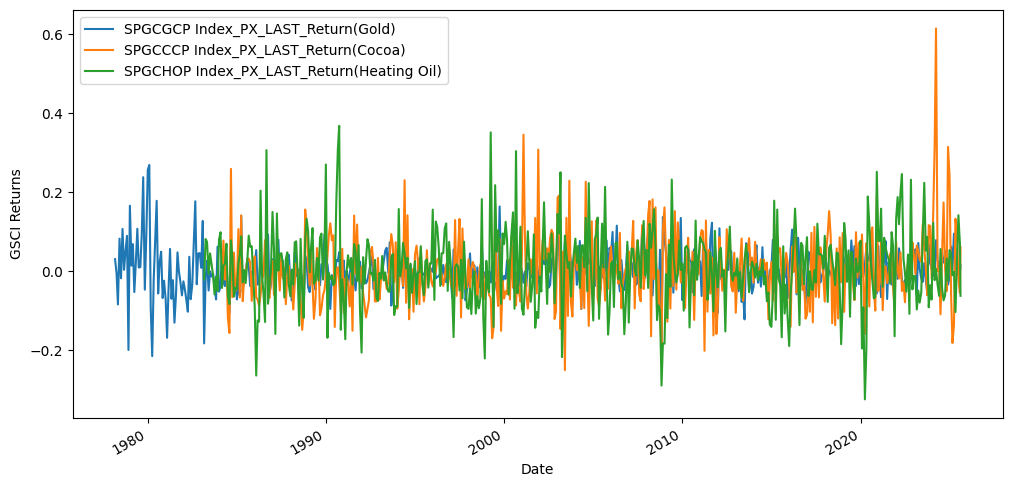
\includegraphics[width=.7\linewidth,height=200pt,width=400pt]{../docs_src/commod_gsci_return.png}
  \end{tabular}
  \caption*{\emph{Sources: Bloomberg, Authors' creation}}
  \label{fig:gsci_commodity_returns}
\end{figure}

\paragraph{Credit Default Swaps}
Our CDS data originate from S\&P Global CDS database (formerly Markit), 
providing daily dealer-contributed curves, reference entity identifiers,
and rich quote metadata for all USD-denominated contracts. 
Our CDS sample follows the constant-risky-duration construction of
\cite{Palhares2012}, a canonical protocol that neutralises maturity roll-over
noise introduced by the 2009 ``Big Bang'' contract change. Raw Markit XR quotes
are first filtered to exclude zero-bid or non-standard contracts, reconciled
with auction recovery data, and rescaled by the risky annuity so that spreads
are comparable across tenors.  The procedure then interpolates missing
maturities, align observations to common month-end fixing dates, and drop quotes
that violate no-arbitrage bounds or sit outside the 1st-99th percentile of the
cross-sectional spread distribution. Open-sourcing this transformation pipeline
provides researchers with CDS excess-return series that are free of roll
discontinuities, stale quote reversals, and documentation clause
inconsistencies.

\subsection{Basis Spread Datasets}

In well-functioning markets, basis spreads---deviations from classical no-arbitrage conditions like covered interest parity (CIP) or put-call parity---should be essentially zero. Persistent or large basis spreads signal that arbitrageurs are unable or unwilling to close riskless profit opportunities, often due to funding frictions or balance sheet constraints. Since the Global Financial Crisis (GFC), researchers have documented several such anomalies across asset classes, and these have important implications for financial stability.
For example, the Covered interest parity (CIP), once ``the closest thing to a physical law in international finance," has been systematically violated since 2008 \cite{Du2018}.
During crisis episodes, these CIP deviations tend to spike sharply, revealing strains in global funding liquidity. For example, in 2008 and again in March 2020, the USD cross-currency basis for major currencies widened dramatically, indicating that foreign institutions were scrambling for dollar liquidity 
\citep{BoardofGovernorsoftheFederalReserveSystem2020}.
Central banks and financial regulators closely monitor and respond to these metrics.
And the Federal Reserve's swap lines are agreements with other central banks to exchange currencies, primarily to provide U.S. dollars to foreign institutions during times of market stress.

In this benchmark repository, we provide code that will allow researchers to replicate a number of basis spreads across several different asset classes. We replicate the basis spreads in \cite{Siriwardane2021}, including spot-futures arbitrage in treasuries, treasury swap arbitrage, TIPS-Treasury arbitrage, CDS-bond basis, CIP arbitrage, spot futures arbitrage in equities, and box arbitrage in equity options.
Each of these basis spreads are, themselves, constructed following methodologies that are well-established in the literature. To validate out replication, I follow the papers recommended in \cite{Siriwardane2021} and replicate key summary statistics from each source paper.



% Please create a paragraph for each basis spread dataset and then, within each paragraph, I don't want to talk about how the portfolios are constructed, but rather I want to talk about the essential cleaning, filtering, and transformations applied, because I want to stress to the reader why, like what is unique or interesting or what is our contribution by open sourcing the cleaning procedure used in this paper. So I guess for each, if you want to establish why is this paper considered canonical, And what are the essential filters and transformations applied by this paper? 

% A full detailed accounting of the cleaning procedure will be given later. These are short introduction glimpses of the why for each Each paragraph should be 2-3 sentences.

\paragraph{Spot-Futures Arbitrage in Treasuries}
Following the Bloomberg cheapest-to-deliver methodology of \citet{Fleckenstein2020} as employed by \citet{Siriwardane2021}, we extract implied risk-free rates from the first-deferred 2-, 5-, 10-, 20- and 30-year Treasury futures.  We retain only days with positive volume, drop the delivery month to avoid the option-to-deliver distortions of \citet{Burghardt2005}, align quotes to the 17:00 ET close, and, per \citet{Barth2021}, match each futures-implied rate to a maturity-matched OIS benchmark-yielding a clean daily Treasury basis series.

\paragraph{Treasury Swap Arbitrage}
We follow \citet{Siriwardane2021} in constructing daily OIS-Treasury swap
spreads: Bloomberg fixed-rate USD OIS quotes for tenors 1-, 2-, 3-, 5-, 10-, 20-
and 30-years are aligned to 17:00 ET and paired with linearly-interpolated
zero-coupon Treasury yields of identical maturities.  Observations with missing
quotes are dropped, delivery-month futures are excluded to sidestep
cheapest-to-deliver noise, and we winsorise the extreme 1\% of spreads; the
resulting series replicates the persistently negative swap spreads documented by
\citet{Jermann2020}, \citet{Du2023}, and \citet{Hanson2023}.

\begin{figure}[h!]
    \centering
    \caption{Treasury Spot-Futures Basis (FTSFR Replication)}
  \begin{tabular}{@{}c@{}}
    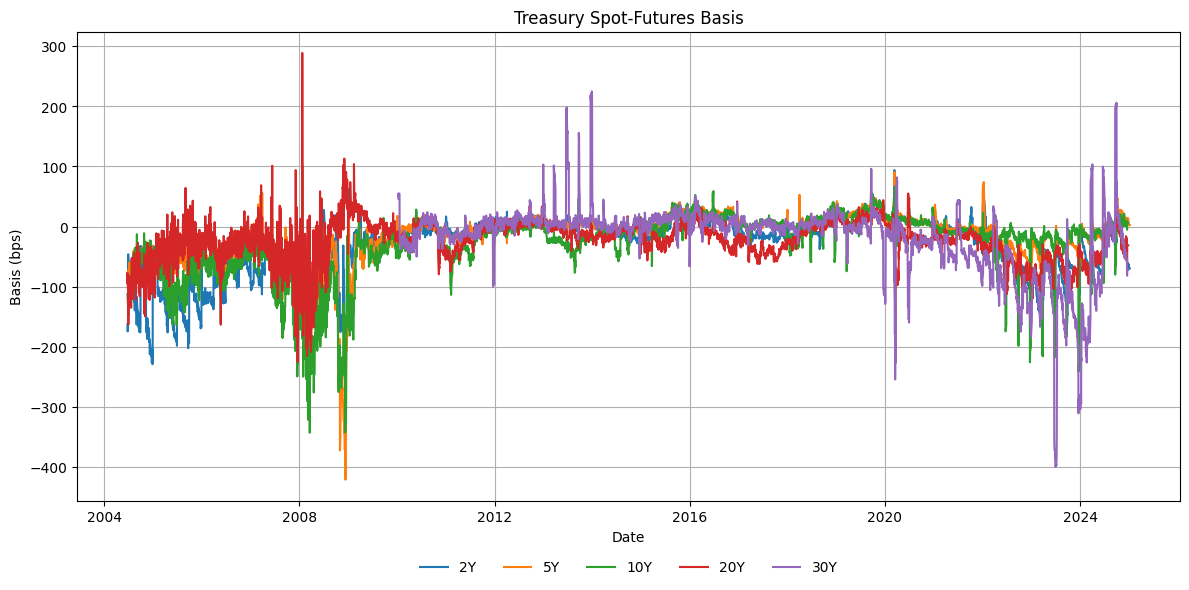
\includegraphics[width=.7\linewidth,height=200pt,width=400pt]{../docs_src/treasury_spot_futures_arbitrage.png}
  \end{tabular}
  \caption*{\emph{Sources: Bloomberg, Authors' creation}}
  \label{fig:treasury_sf_basis}
\end{figure}


\begin{figure}[h!]
  \centering
  \caption{Treasury Swap Arbitrage spreads}
  \begin{tabular}{@{}c@{}}
    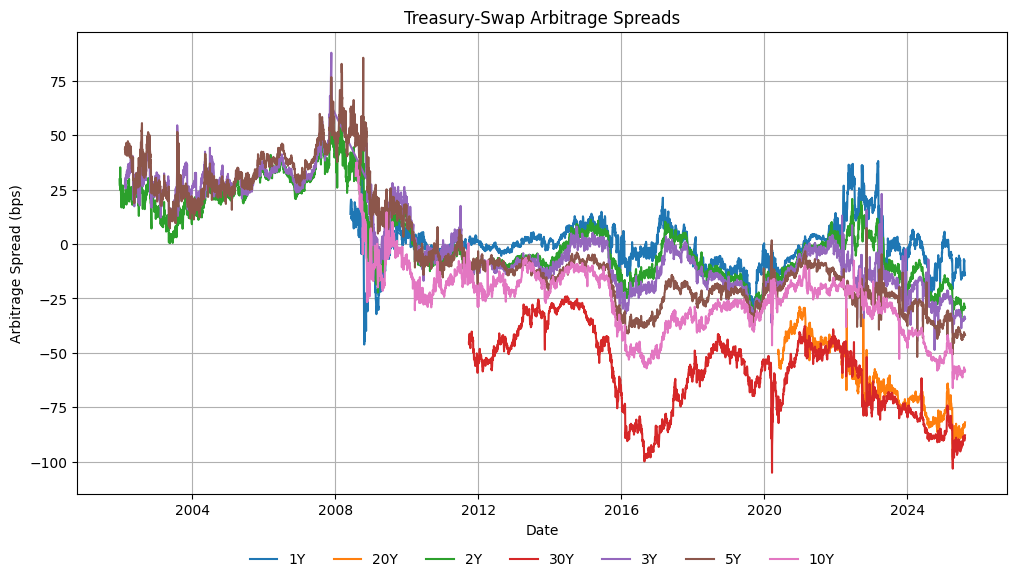
\includegraphics[width=.7\linewidth,height=200pt,width=400pt]{../docs_src/treasury_swap_arbitrage_spreads.png}
  \end{tabular}
  \caption*{\emph{Sources: Bloomberg, Authors' creation}}
  \label{fig:treasury_swap_arbitrage}
\end{figure}


\paragraph{TIPS-Treasury Arbitrage}
Replicating \citet{Fleckenstein2014} as implemented in \citet{Siriwardane2021}, we splice Federal Reserve zero-coupon TIPS yields with Bloomberg constant-maturity inflation-swap rates to create synthetic nominal yields, then difference these against equal-maturity zero-coupon Treasury yields for the 2-, 5-, 10- and 20-year tenors.  We exclude days with missing swap quotes or illiquid TIPS issues, drop outliers beyond the extreme 1\%, and harmonise all series to 17:00 ET closes to obtain a clean daily TIPS-Treasury basis series.

\begin{figure}[h!]
    \caption{TIPS-Treasury Arbitrage spreads.}
  \centering
  \begin{tabular}{@{}c@{}}
    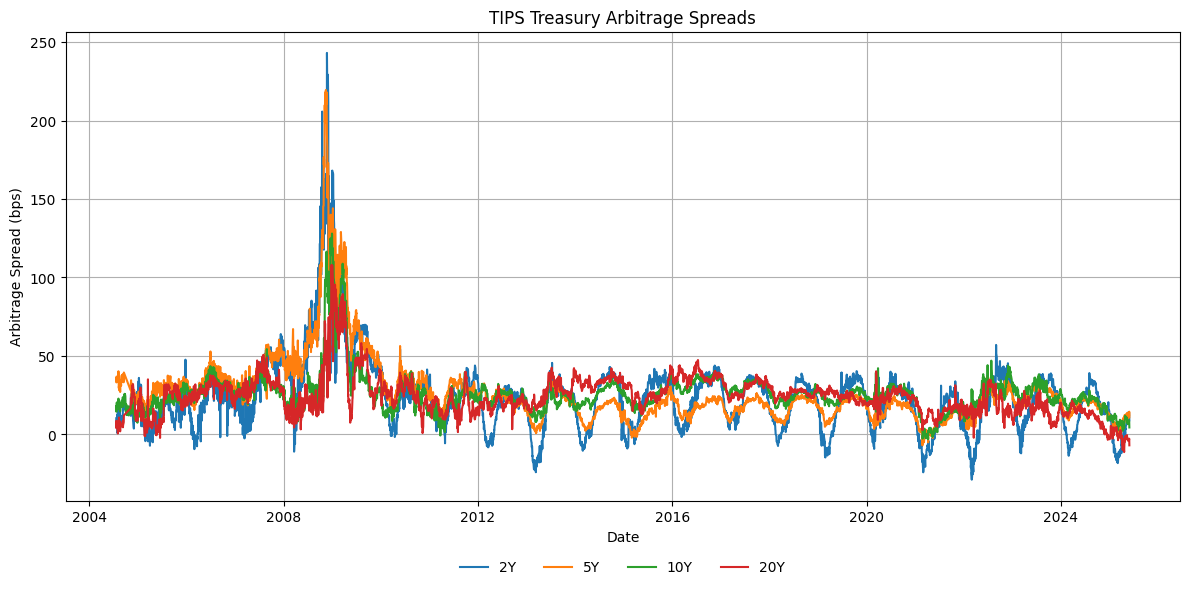
\includegraphics[width=.7\linewidth,height=200pt,width=400pt]{../docs_src/tips_treasury_arbitrage_spreads.png}
  \end{tabular}
  \caption*{\emph{Sources: Bloomberg, Authors' creation}}
  \label{fig:tips_treasury_basis}
\end{figure}

\paragraph{CDS-Bond Basis}
% TODO: Check this paragraph.
% we should be doing duration matching, added that in
% i am removing RFR when over 1, representing 100%
% - Vincent
Leveraging the daily Markit pricing files used by \citet{Siriwardane2021}, we link cash bonds to matching single-name CDS and compute the basis after (i) retaining only USD-denominated senior unsecured issues with fixed coupons and 1-10-year maturities, (ii) discarding quotes with prices below 50¢, zero bids, or stale timestamps, and (iii) mapping each bond to a duration-matched CDS par spread via cubic-spline interpolation.  We further exclude callable/convertible structures, winsorise extreme 100\% bases, and require each bond to appear in our cleaned version of the public FINRA TRACE dataset to guarantee tradability, yielding a high-quality daily series that mirrors the investment-grade and high-yield bases reported in the original study.


% TODO: Vincent and Alex
% 1. Change y axis label so that it shows percents. Change rfr to "Implied Risk-Free Rate (percent)"
% 2. Get rid of Title in the plot. I can add the title in the LaTeX code myself.
% 3. Get rid of Rating "2", since Rating 2 is the weird hybrid one.
% 4. Rename rating 0 to "High Yield" and rating 1 to "Investment Grade"
\begin{figure}[h!]
    \centering
    \caption{CDS Arbitrage spreads}
  \begin{tabular}{@{}c@{}}
    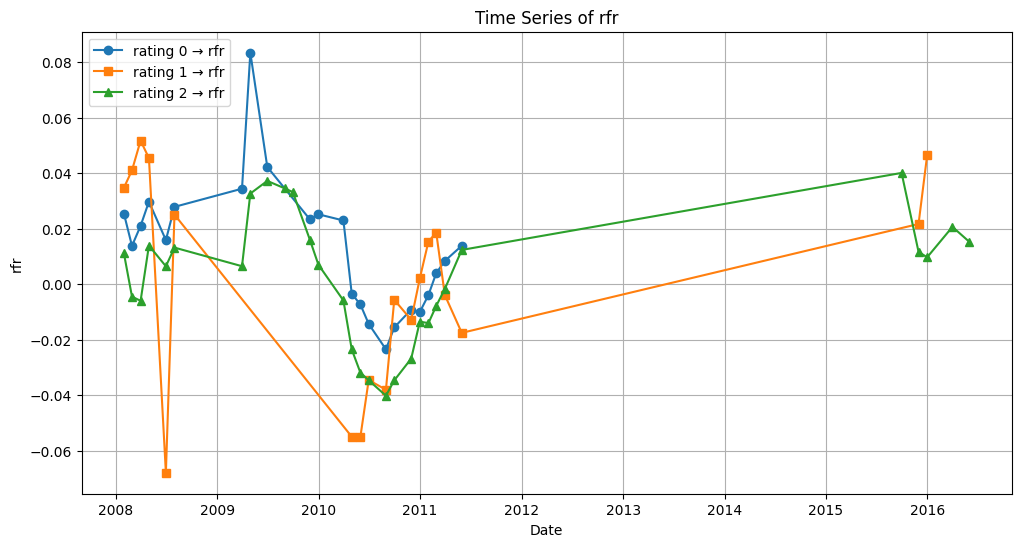
\includegraphics[width=.7\linewidth]{../docs_src/CDS_replicate.png}
  \end{tabular}
  \caption*{\emph{Sources: S\&P Global, WRDS TRACE,Authors' creation}}
  \label{fig:cds_basis}
\end{figure}

\paragraph{CIP Arbitrage}
For Covered Interest Parity (CIP) we replicate the G10 series in \citet{Du2018}, merging Bloomberg mid-quotes for spot rates, 3-month forwards, and maturity-matched OIS curves.  Core filters rescale forward points (and invert USD-quoted pairs), synchronise all legs to the 17:00 ET close while dropping holiday or stale quotes, and winsorise the extreme 1\% of annualised spreads with spline interpolation for any missing OIS tenors to remove scaling, timing, and rate-sourcing distortions.

\begin{figure}[h!]
    \centering
    \caption{CIP Arbitrage spreads}
  \begin{tabular}{@{}c@{}}
    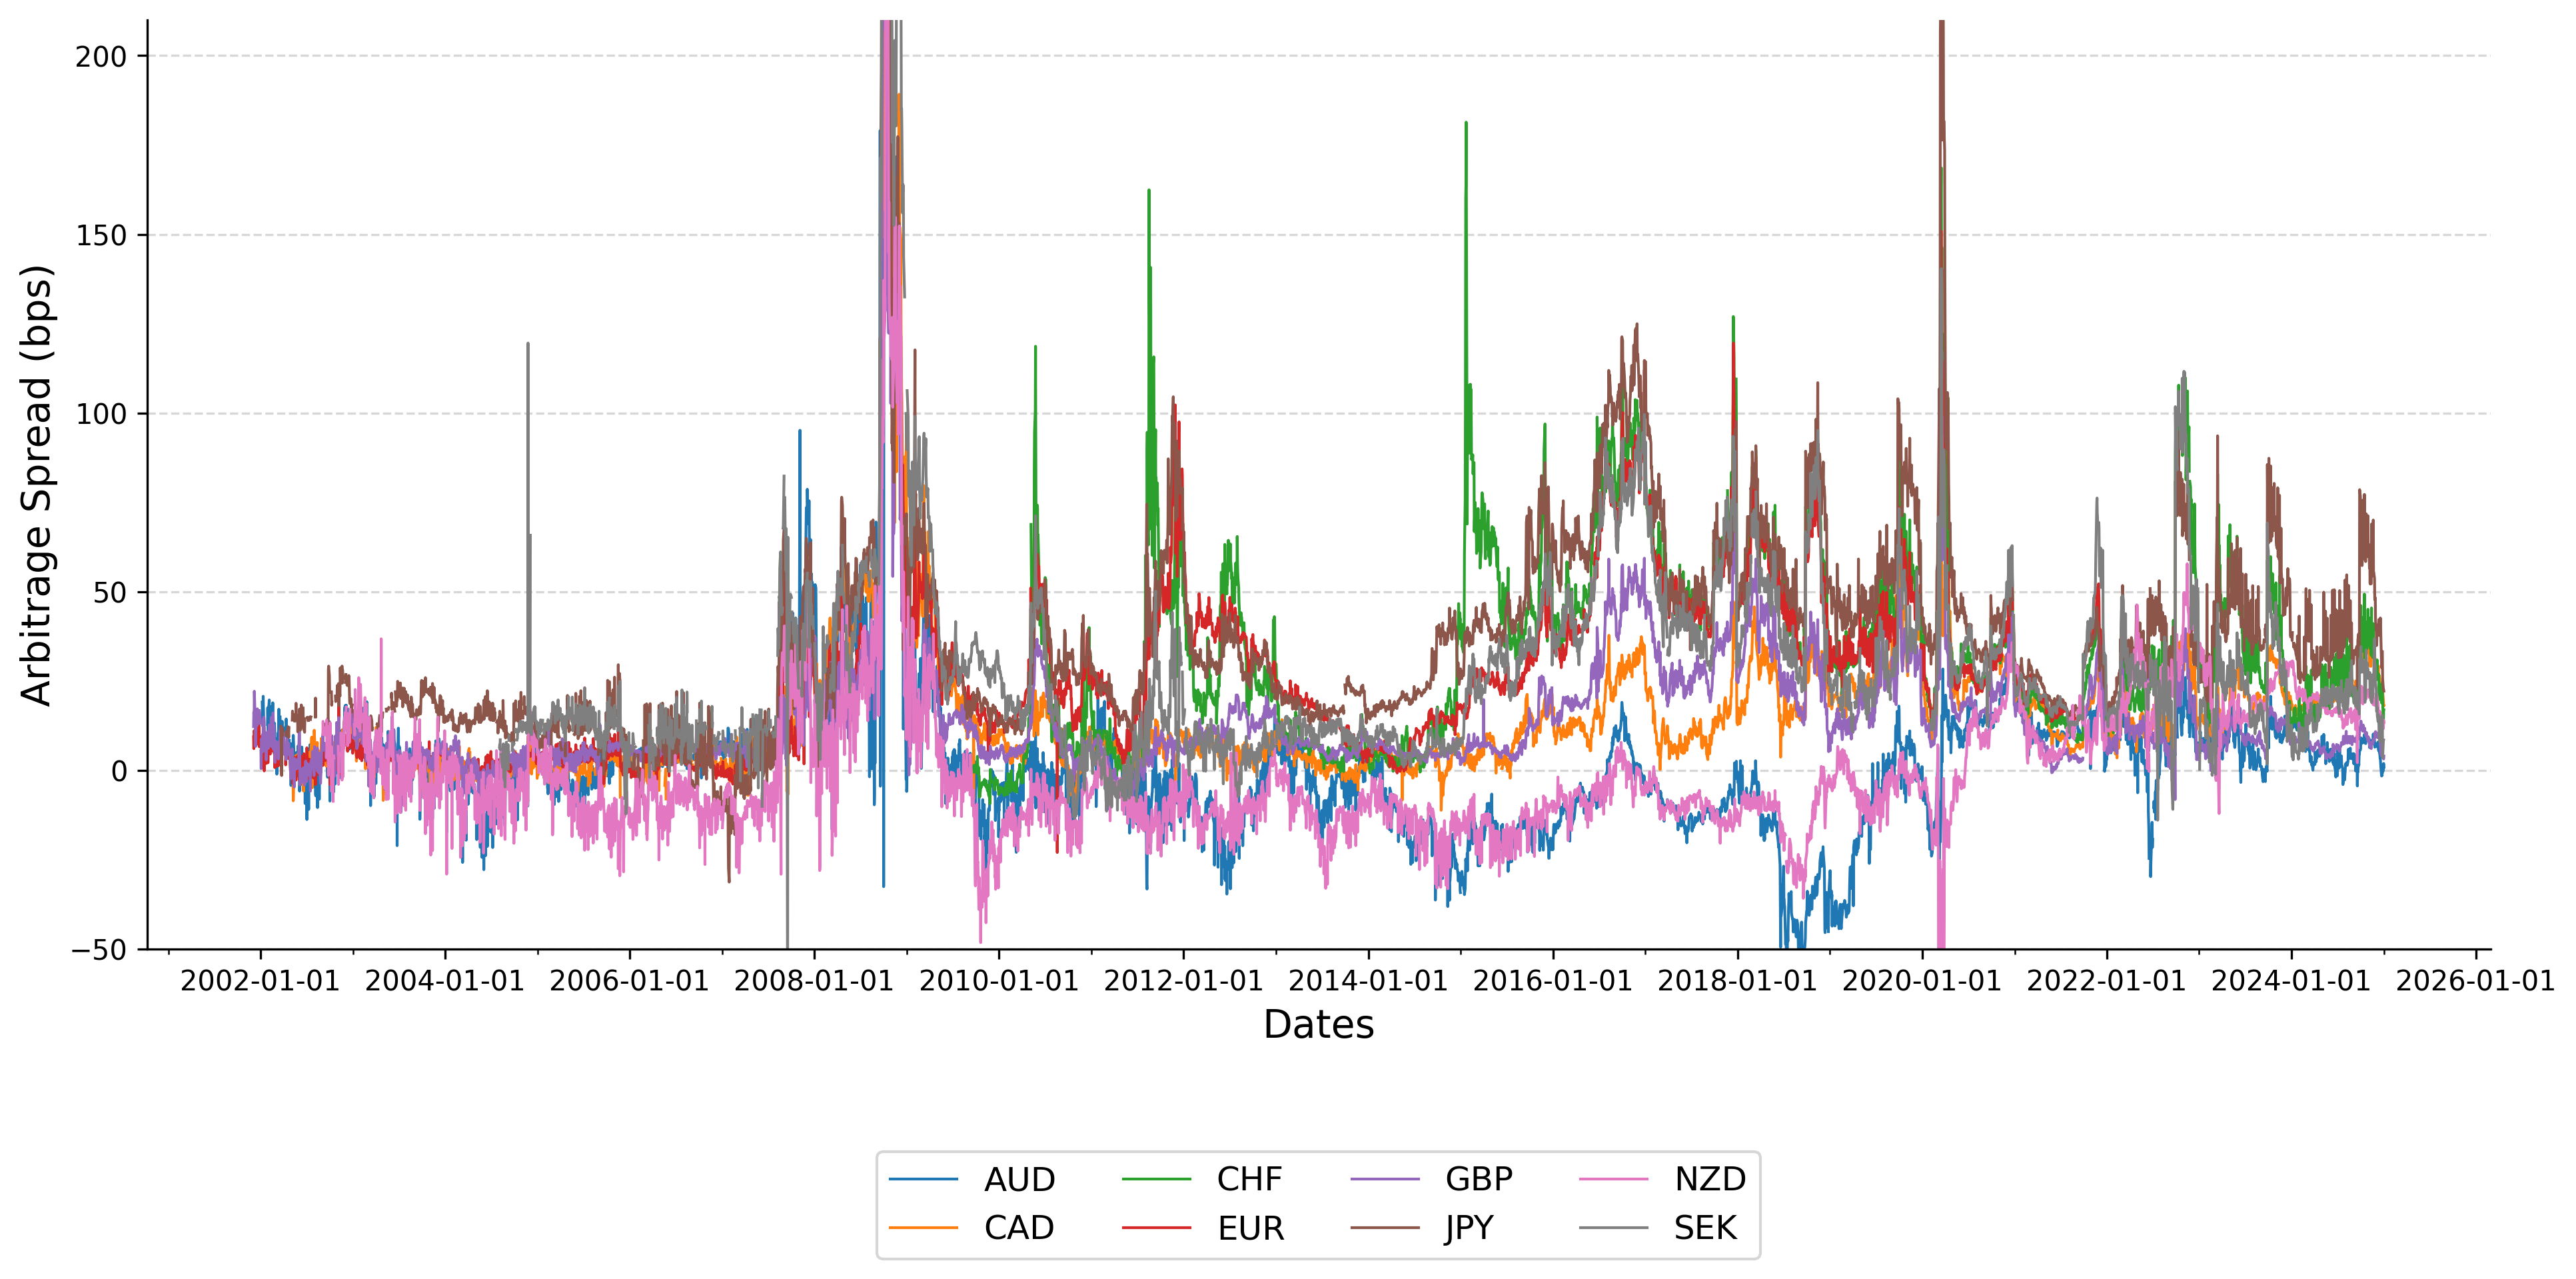
\includegraphics[width=.7\linewidth]{../docs_src/CIP_replicate.png}
  \end{tabular}
  \caption*{\emph{Sources: Bloomberg, Authors' creation}}
  \label{fig:cip_basis}
\end{figure}

% \paragraph{Spot Futures Arbitrage in Equities}

% Following the equity basis recipe of \citet{Hazelkorn2023}, we construct implied forward rates from nearby and first-deferred S\&P 500, Dow Jones, and Nasdaq 100 futures to avoid measurement error from asynchronous spot and futures market closes. We proxy for expected dividends using realized dividends from Bloomberg. The final arbitrage spread is the difference between this futures-implied rate and the 3-month OIS rate, which serves as a clean risk-free benchmark.

% \paragraph{Box Arbitrage in Equity Options}
% For box spread arbitrage, we follow the methodology of \citet{VanBinsbergen2022} to extract a risk-free rate implied by S\&P 500 (SPX) index options. Their approach uses a cross-sectional regression of put-call price differences on strike prices, which cleverly avoids the need to explicitly estimate dividends. We use their publicly available daily median implied rates and extend the series using their exact methodology on recent minute-level CBOE data. The final arbitrage spread is the difference between this options-implied rate and a maturity-matched OIS rate.

\subsection{Other Financial Data}

\paragraph{Call Report}
Bank variables come directly from the Drechsler-Savov-Schnabl Call Report panel, \citep{Drechsler2017}. Their WRDS code downloads FFIEC 031/041 series and harmonizes item definitions across form changes (e.g., RCFD$\rightarrow$RCON after 2011; time-deposit thresholds shifting from \$100k to \$250k in 2010), converts YTD income/expense to quarterly flows, handles pre-1982 semiannual filers, and builds consistent series for assets, loans, deposits, and interest expense. We use their released bank-level file (1976-2020) and construct our ratios (e.g., cash/liquidity, leverage). 

\paragraph{Intermediary Capital Risk Factors}
We use the series released by \citet{He2017}\footnote{See \url{https://zhiguohe.net/data-and-empirical-patterns/intermediary-capital-ratio-and-risk-factor/}}. He, Kelly, and Manela (HKM) construct the intermediary capital ratio for primary dealer holding companies as aggregate market equity divided by aggregate market equity plus book debt, matching the dealer list to public holding companies in CRSP/Compustat/Datastream. The "intermediary capital risk factor" is the AR(1) innovation in the capital ratio scaled by the lagged ratio. We simply align the published monthly (and post-2000 daily) series to our panel and do not re-estimate the factor.


\paragraph{Yield Curve}
We take the off-the-shelf Gürkaynak-Sack-Wright (GSW) nominal zero-coupon curve published by the Federal Reserve \citep{Gurkaynak2007}. GSW fit a smooth Nelson-Siegel-Svensson curve to off-the-run Treasury notes and bonds (bills/FRNs and on-the-run issues excluded). The six-parameter Svensson model is used post-1980 and Nelson-Siegel before 1980. We simply reshape the released zero-coupon yields to our panel. 


\section{Forecasting Methodology}
\label{sec:methodology}

% TODO: Define forecasting approach following Monash template
% - Justify choice of error metrics
% - Select baseline forecasting models
% - Define evaluation methodology

In this section, we describe our forecasting methodology, including the baseline models used, data preprocessing procedures, and error metrics employed for evaluation. Our approach is designed to establishing reliable baseline performance measures and provide fair comparisons across diverse financial time series. We first present our selection of forecasting models spanning classical statistical methods and modern machine learning approaches. We then detail our data preprocessing and filtering methodology, which ensures consistent treatment across all models and datasets. Finally, we define our comprehensive suite of error metrics, chosen to provide complementary perspectives on forecasting performance while enabling meaningful comparisons across different asset classes and time series characteristics.

\subsection{Baseline Models}
% Traditional, ML, and Deep Learning models
% TODO: Arsh: Add bullet points provide a short 2-3 sentence description of each model. What is the basic idea behind each model? Who developed it? What package are we using to implement it? 

The models presented in this section are not intended to provide an exhaustive review of all available forecasting methods, nor are they estimated to their fully optimized specifications. Rather, we select a representative set of models from different areas of statistics and machine learning---including classical statistical methods, traditional machine learning approaches, and modern deep learning architectures---and apply them with minimal tuning to establish baseline forecasting performance. This approach allows us to demonstrate the utility of our benchmark datasets while providing reasonable comparative baselines that researchers can build upon. The primary emphasis of this paper is to provide high-quality, standardized benchmark datasets that others can readily use to evaluate their own forecasting models and methodologies. All classical statistical and modern machine learning models are implemented using the \texttt{statsforecast} and \texttt{neuralforecast} packages by Nixtla for Python, ensuring reproducible and standardized implementations.

% \begin{itemize}
%     \item ARIMA: Standard Autoregressive Integrated Moving Average model based on the statsmodel implementation.\cite{Box2013}
%     \begin{itemize}
%         \item \textbf{Forecasting Type: }Local
%         \item \textbf{Package Used: }\texttt{\href{https://unit8co.github.io/darts/generated_api/darts.models.forecasting.arima.html}{darts}}
%     \end{itemize}
%     \item ETS: We use the Holt-Winter's exponential smoothing model\cite{Winters1960}. % Please add this citation from the URL: https://www.sciencedirect.com/science/article/abs/pii/S0169207003001134
%     \begin{itemize}
%         \item \textbf{Forecasting Type: }Local
%         \item \textbf{Package Used: }\texttt{\href{https://unit8co.github.io/darts/generated_api/darts.models.forecasting.exponential_smoothing.html}{darts}}
%     \end{itemize}
%     \item Simple Exponential Smoothing: simple exponential moving average on a time-series\cite{Brown2004}.
%     \begin{itemize}
%         \item \textbf{Forecasting Type: }Local
%         \item \textbf{Package Used: }\texttt{\href{https://unit8co.github.io/darts/generated_api/darts.models.forecasting.exponential_smoothing.html}{darts}}
%     \end{itemize}
%     \item TBATS: Uses Box-Cox transformations, ARMA error corrections and Fourier representations\cite{DeLivera2011a}.
%     \begin{itemize}
%         \item \textbf{Forecasting Type: }Local
%         \item \textbf{Package Used: }\texttt{\href{https://unit8co.github.io/darts/generated_api/darts.models.forecasting.sf_tbats.html}{darts}}
%     \end{itemize}
%     \item Theta: Splits a time-series into multiple Theta lines which are extrpolated separately and their combination is taken as the forecast\cite{Assimakopoulos2000}.
%     \begin{itemize}
%         \item \textbf{Forecasting Type: }Local
%         \item \textbf{Package Used: }\texttt{\href{https://unit8co.github.io/darts/generated_api/darts.models.forecasting.theta.html\#darts.models.forecasting.theta.Theta}{darts}}
%     \end{itemize}
%     \item Prophet: decomposable time-series model similar to Generalized Additive Model(GAM) developed by Facebook\cite{Taylor2018}.
%     \begin{itemize}
%         \item \textbf{Forecasting Type: }Local
%         \item \textbf{Package Used: }\texttt{\href{https://unit8co.github.io/darts/generated_api/darts.models.forecasting.prophet_model.html}{darts}}
%     \end{itemize}
%     \item PR (Pooled Regression): Generic gaussian linear model\cite{Trapero2015}
%     \begin{itemize}
%         \item \textbf{Forecasting Type: }Global
%         \item \textbf{Package Used: }\texttt{\href{https://unit8co.github.io/darts/generated_api/darts.models.forecasting.sklearn_model.html\#darts.models.forecasting.sklearn_model.SKLearnModel}{darts}} and \texttt{\href{https://scikit-learn.org/stable/modules/generated/sklearn.linear_model.TweedieRegressor.html\#sklearn.linear_model.TweedieRegressor}{scikit-learn}}
%     \end{itemize}
%     \item CatBoost: Gradient boosting algorithm for dealing with categorical data and a leaf value calculation trick which reduces overfitting\cite{Prokhorenkova}.
%     \begin{itemize}
%         \item \textbf{Forecasting Type: }Global
%         \item \textbf{Package Used: }\texttt{\href{https://unit8co.github.io/darts/generated_api/darts.models.forecasting.catboost_model.html}{darts}}
%     \end{itemize}
%     \item FFNN (Feed-Forward Neural Network): Simple neural network which is a collection of weight tensors with activation functions in between\cite{Goodfellow2016}.
%     \begin{itemize}
%         \item \textbf{Forecasting Type: }Global
%         \item \textbf{Package Used: }\texttt{\href{https://ts.gluon.ai/stable/api/gluonts/gluonts.torch.model.simple_feedforward.html}{gluonts}} with \texttt{torch} backend
%     \end{itemize}
%     \item Transformer: A deep network architecture utilising attention mechanisms for deducing dependencies in the input and the output\cite{Vaswani2017}.
%     \begin{itemize}
%         \item \textbf{Forecasting Type: }Global
%         \item \textbf{Package Used: }\texttt{\href{https://unit8co.github.io/darts/generated_api/darts.models.forecasting.transformer_model.html}{darts}}
%     \end{itemize}
%     \item DeepAR: An Autoregressive Recurrent Neural Network(RNN) with Long Short-Term Memory(LSTM).\cite{Salinas2020}
%     \begin{itemize}
%         \item \textbf{Forecasting Type: }Global
%         \item \textbf{Package Used: }\texttt{\href{https://ts.gluon.ai/stable/api/gluonts/gluonts.torch.model.deepar.module.html}{gluonts}} with \texttt{torch} backend
%     \end{itemize}
%     \item WaveNet: Dilated deep neural network employing convolution layers. Originally made to generate sound waveforms\cite{Oord2016} but adapted to use in forecasting. % PLEASE ADD CITATION FROM URL: https://arxiv.org/abs/1703.04691
%     \begin{itemize}
%         \item \textbf{Forecasting Type: }Global
%         \item \textbf{Package Used: }\texttt{\href{https://ts.gluon.ai/stable/api/gluonts/gluonts.torch.model.wavenet.html}{gluonts}} with \texttt{torch} backend
%     \end{itemize}
%     \item D-Linear: Transformer-based deep model which is a combination of a decomposition scheme with linear layers\cite{Zeng2022}.
%     \begin{itemize}
%         \item \textbf{Forecasting Type: }Global
%         \item \textbf{Package Used: }\texttt{\href{https://unit8co.github.io/darts/generated_api/darts.models.forecasting.dlinear.html}{darts}}
%     \end{itemize}
%     \item N-Linear: Transformer-based deep model which addresses distribution shifts in the dataset by using a normalization trick\cite{Zeng2022}.
%     \begin{itemize}
%         \item \textbf{Forecasting Type: }Global
%         \item \textbf{Package Used: }\texttt{\href{https://unit8co.github.io/darts/generated_api/darts.models.forecasting.nlinear.html}{darts}}
%     \end{itemize}
%     \item N-BEATS: Deep neural network with fully-connected layers along with residual links\cite{Oreshkin2020}.
%     \begin{itemize}
%         \item \textbf{Forecasting Type: }Global
%         \item \textbf{Package Used: }\texttt{\href{https://unit8co.github.io/darts/generated_api/darts.models.forecasting.nbeats.html}{darts}}
%     \end{itemize}
%     \item N-HiTS: Enhances N-BEATS by using multi-rate data sampling and multi-scale interpolation\cite{Challu2022}.
%     \begin{itemize}
%         \item \textbf{Forecasting Type: }Global
%         \item \textbf{Package Used: }\texttt{\href{https://unit8co.github.io/darts/generated_api/darts.models.forecasting.nhits.html\#darts.models.forecasting.nhits.NHiTSModel}{darts}}
%     \end{itemize}
%     \item Autoformer: Transformer-based deep network employing decomposition and Auto-Correlation\cite{Wu2021}.
%     \begin{itemize}
%         \item \textbf{Forecasting Type: }Global
%         \item \textbf{Package Used: }Nixtla's \texttt{\href{https://nixtlaverse.nixtla.io/neuralforecast/models.autoformer.html}{neuralforecast}}
%     \end{itemize}
%     \item Informer: Transformer-based architecture using a ProbSparse self-attention mechanism and a generative-style decoder among other techniques\cite{Zhou2020}.
%     \begin{itemize}
%         \item \textbf{Forecasting Type: }Global
%         \item \textbf{Package Used: }Nixtla's \texttt{\href{https://nixtlaverse.nixtla.io/neuralforecast/models.informer.html}{neuralforecast}}
%     \end{itemize}
%     \item PatchTST: Transformer-based model breaking a time series into a collection of patches used as tokens and utilises channel independence\cite{Nie2022}.
%     \begin{itemize}
%         \item \textbf{Forecasting Type: }Global
%         \item \textbf{Package Used: }\texttt{\href{https://ts.gluon.ai/stable/api/gluonts/gluonts.torch.model.patch_tst.html}{gluonts}} with \texttt{torch} backend
%     \end{itemize}
%     \item Temporal Fusion Transformer: Transformer-based model employing recurrent layers and self-attention layers with a focus on interpretablility\cite{Lim2021}
%     \begin{itemize}
%         \item \textbf{Forecasting Type: }Global
%         \item \textbf{Package Used: }\texttt{\href{https://ts.gluon.ai/stable/api/gluonts/gluonts.torch.model.tft.module.html}{gluonts}} with \texttt{torch} backend
%     \end{itemize}
%     \item Time-series Dense Encoder(TiDE): Multi-layer perceptron based architecture utilising encoder and decoder blocks\cite{Das2023a}.
%     \begin{itemize}
%         \item \textbf{Forecasting Type: }Global
%         \item \textbf{Package Used: }\texttt{\href{https://unit8co.github.io/darts/generated_api/darts.models.forecasting.tide_model.html}{darts}}
%     \end{itemize}
%     \item TimesFM: Pre-trained transformer-based decoder-only deep model utilising patches similar to PatchTST\cite{Das2023}.
%     \begin{itemize}
%         \item \textbf{Forecasting Type: }Global
%         \item \textbf{Package Used: }\texttt{\href{https://github.com/google-research/timesfm}{timesfm}} python package
%     \end{itemize}
% \end{itemize}


\begin{itemize}
    \item Theta: Splits a time-series into multiple Theta lines which are extrpolated separately and their combination is taken as the forecast, following \cite{Assimakopoulos2000}.
    \item Simple Exponential Smoothing: simple exponential moving average on a time-series, following \cite{Brown2004}.
    \item AutoARIMA: Autoregressive Integrated Moving Average model with automatic parameter selection, where the algorithm automatically determines the optimal values for the ARIMA(p,d,q) parameters through stepwise search and information criteria, following \cite{Box2013} and \cite{Hyndman2008}.
    \item DeepAR: An Autoregressive Recurrent Neural Network(RNN) with Long Short-Term Memory(LSTM), following \cite{Salinas2020}.
    \item N-BEATS: Deep neural network with fully-connected layers along with residual links, following \cite{Oreshkin2020}.
    \item N-HiTS: Enhances N-BEATS by using multi-rate data sampling and multi-scale interpolation, following \cite{Challu2022}.
    \item D-Linear: Transformer-based deep model which is a combination of a decomposition scheme with linear layers, following \cite{Zeng2022}.
    \item N-Linear: Transformer-based deep model which addresses distribution shifts in the dataset by using a normalization trick, following \cite{Zeng2022}.
    % \item ETS: We use the Holt-Winter's exponential smoothing model, following \cite{Winters1960}. % Please add this citation from the URL: https://www.sciencedirect.com/science/article/abs/pii/S0169207003001134
    % \item TBATS: Uses Box-Cox transformations, ARMA error corrections and Fourier representations\cite{DeLivera2011a}.
    % \begin{itemize}
    %     \item \textbf{Forecasting Type: }Local
    %     \item \textbf{Package Used: }\texttt{\href{https://unit8co.github.io/darts/generated_api/darts.models.forecasting.sf_tbats.html}{darts}}
    % \end{itemize}
    % \item Prophet: decomposable time-series model similar to Generalized Additive Model(GAM) developed by Facebook\cite{Taylor2018}.
    % \begin{itemize}
    %     \item \textbf{Forecasting Type: }Local
    %     \item \textbf{Package Used: }\texttt{\href{https://unit8co.github.io/darts/generated_api/darts.models.forecasting.prophet_model.html}{darts}}
    % \end{itemize}
    % \item PR (Pooled Regression): Generic gaussian linear model\cite{Trapero2015}
    % \begin{itemize}
    %     \item \textbf{Forecasting Type: }Global
    %     \item \textbf{Package Used: }\texttt{\href{https://unit8co.github.io/darts/generated_api/darts.models.forecasting.sklearn_model.html\#darts.models.forecasting.sklearn_model.SKLearnModel}{darts}} and \texttt{\href{https://scikit-learn.org/stable/modules/generated/sklearn.linear_model.TweedieRegressor.html\#sklearn.linear_model.TweedieRegressor}{scikit-learn}}
    % \end{itemize}
    % \item CatBoost: Gradient boosting algorithm for dealing with categorical data and a leaf value calculation trick which reduces overfitting\cite{Prokhorenkova}.
    % \begin{itemize}
    %     \item \textbf{Forecasting Type: }Global
    %     \item \textbf{Package Used: }\texttt{\href{https://unit8co.github.io/darts/generated_api/darts.models.forecasting.catboost_model.html}{darts}}
    % \end{itemize}
    % \item FFNN (Feed-Forward Neural Network): Simple neural network which is a collection of weight tensors with activation functions in between\cite{Goodfellow2016}.
    % \begin{itemize}
    %     \item \textbf{Forecasting Type: }Global
    %     \item \textbf{Package Used: }\texttt{\href{https://ts.gluon.ai/stable/api/gluonts/gluonts.torch.model.simple_feedforward.html}{gluonts}} with \texttt{torch} backend
    % \end{itemize}
    \item Transformer: A deep network architecture utilising attention mechanisms for deducing dependencies in the input and the output, following \cite{Vaswani2017}.
    \item Time-series Dense Encoder (TiDE): Multi-layer perceptron based architecture utilising encoder and decoder blocks, following \cite{Das2023a}.
    \item KAN: Kolmogorov-Arnold Networks replace fixed activations with learnable spline-based functions on edges instead of nodes, inspired by the Kolmogorov-Arnold representation theorem. This design improves both accuracy and interpretability, allowing smaller networks to outperform larger MLPs in regression and PDE tasks, following \cite{Liu2025}.

\end{itemize}


\subsection{Data Preprocessing}

To ensure fair model comparisons, our forecasting system applies consistent filtering and data preprocessing across all models and datasets. Table~\ref{tab:filtered_dataset_stats} shows the impact of this filtering, displaying entity counts and median time series lengths before and after preprocessing. 

\paragraph{Filtering Methodology and Fairness Guarantees.} Our filtering procedure addresses fundamental differences between statistical forecasting methods (which can handle very short or irregular time series) and neural forecasting methods (which require sufficient data for training and validation). To ensure fairness, we implement entity-based forecast horizon calculation that adapts to each dataset's characteristics rather than using a global threshold. For datasets with median entity lengths below 100 observations, we calculate the forecast horizon as a percentage of the median entity length with a minimum buffer of 6 observations. For longer time series, we use seasonality-aware thresholds (e.g., 24 observations for monthly data to capture two full seasonal cycles). Crucially, we protect small datasets by implementing a hard cap: any dataset beginning with 10 or fewer entities is exempt from length-based filtering to prevent complete elimination of entire asset classes.

\paragraph{Technical Implementation.} The filtering system operates in two stages. First, we apply standardized data cleaning using forward-only fill strategies to handle missing values consistently across all models, avoiding the artificial length inflation that backward-filling can create when combined with our gap-filling procedures. Second, we filter time series based on minimum length requirements calculated per entity rather than globally, ensuring that the diverse time series characteristics within each dataset (e.g., securities with different listing dates) are handled appropriately. All models-whether StatsForecast implementations like Naive, Seasonal Naive, or Theta, or NeuralForecast implementations like NBEATs, NHiTS, or Transformer variants-receive identical filtered datasets for training and evaluation.

\paragraph{Impact and Necessity.} This preprocessing is essential because neural methods require sufficient observations for training, validation splits, and convergence, while statistical methods can theoretically operate on very short series but may produce unreliable forecasts without adequate historical context. The filtering has varying impact across asset classes: portfolio-level datasets (which are typically well-maintained) show minimal changes, while disaggregated datasets show substantial filtering due to the presence of shorter-lived securities or incomplete data coverage. For instance, individual CDS contracts are filtered from 6,508 to 6,388 entities (98\% retention), while the commodities dataset requires more aggressive filtering from 23 to 4 entities due to data availability constraints. This systematic approach ensures that performance comparisons reflect true forecasting capability rather than artifacts of inconsistent data preprocessing.

\begin{table}[htbp]
\centering
\caption{Impact of Filtering on Dataset Statistics}
\label{tab:filtered_dataset_stats}
% Filtered Dataset Statistics Summary - tabular content only
% Generated automatically by create_filtered_dataset_statistics.py
\footnotesize
\setlength{\tabcolsep}{1.0pt}
\renewcommand{\arraystretch}{0.9}
\begin{tabular}{@{}llrrrrlll@{}}
\toprule
 & Frequency & \begin{tabular}[c]{@{}r@{}}Entities\\Before\end{tabular} & \begin{tabular}[c]{@{}r@{}}Entities\\After\end{tabular} & \begin{tabular}[c]{@{}r@{}}Median Length\\Before\end{tabular} & \begin{tabular}[c]{@{}r@{}}Median Length\\After\end{tabular} & Min Date & Max Date \\
\midrule
\multicolumn{8}{l}{\textbf{Basis Spreads}} \\
CDS-Bond & Monthly & 3398 & 3314 & 199 & 201 & 2002-09-30 & 2022-09-30 \\
CIP & Monthly & 8 & 8 & 224 & 224 & 2001-12-04 & 2025-02-22 \\
TIPS-Treasury & Monthly & 4 & 4 & 200 & 200 & 2004-07-21 & 2025-05-21 \\
Treasury-SF & Monthly & 5 & 5 & 204 & 204 & 2004-06-23 & 2024-12-23 \\
Treasury-Swap & Monthly & 7 & 7 & 166 & 166 & 2001-12-20 & 2025-08-04 \\
\midrule
\multicolumn{8}{l}{\textbf{Returns (Portfolios)}} \\
CDS Portfolio & Monthly & 20 & 20 & 220 & 220 & 2001-01-01 & 2023-12-01 \\
Corporate Portfolio & Monthly & 10 & 10 & 193 & 193 & 2002-08-31 & 2022-09-30 \\
FF25 Size-BM & Daily & 25 & 25 & 28928 & 28928 & 1926-07-01 & 2025-06-30 \\
SPX Options Portfolios & Monthly & 18 & 18 & 230 & 230 & 1996-01-31 & 2019-12-31 \\
Treasury Portfolio & Monthly & 10 & 10 & 532 & 532 & 1970-01-31 & 2025-06-30 \\
\midrule
\multicolumn{8}{l}{\textbf{Returns (Disaggregated)}} \\
CDS Contract & Monthly & 6508 & 6388 & 215 & 217 & 2001-01-01 & 2023-12-01 \\
CRSP Stock & Monthly & 26719 & 26474 & 436 & 440 & 1926-01-30 & 2024-12-31 \\
CRSP Stock (ex-div) & Monthly & 26719 & 26474 & 436 & 440 & 1926-01-30 & 2024-12-31 \\
Commodity & Monthly & 23 & 4 & 399 & 555 & 1970-01-30 & 2025-07-30 \\
Corporate Bond & Monthly & 23445 & 22146 & 144 & 154 & 2002-08-31 & 2022-09-30 \\
FX & Monthly & 9 & 9 & 222 & 222 & 1999-02-09 & 2025-02-23 \\
Treasury Bond & Monthly & 2033 & 1951 & 234 & 250 & 1970-01-31 & 2025-06-30 \\
\midrule
\multicolumn{8}{l}{\textbf{Other}} \\
BHC Cash Liquidity & Quarterly & 13529 & 13279 & 136 & 136 & 1976-03-31 & 2020-03-31 \\
BHC Leverage & Quarterly & 13520 & 13270 & 136 & 136 & 1976-03-31 & 2020-03-31 \\
Bank Cash Liquidity & Quarterly & 23834 & 23816 & 168 & 168 & 1976-03-31 & 2020-03-31 \\
Bank Leverage & Quarterly & 22940 & 22927 & 168 & 168 & 1976-03-31 & 2020-03-31 \\
HKM All Factor & Monthly & 4 & 4 & 412 & 412 & 1970-01-01 & 2012-12-01 \\
HKM Daily Factor & Daily & 4 & 4 & 5534 & 5534 & 2000-01-03 & 2018-12-11 \\
HKM Monthly Factor & Monthly & 4 & 4 & 469 & 469 & 1970-01-01 & 2018-11-01 \\
Treasury Yield Curve & Daily & 30 & 30 & 13180 & 13180 & 1961-06-14 & 2025-08-08 \\
\bottomrule
\end{tabular}
\vspace{0.1cm}
\begin{minipage}{\textwidth}
\scriptsize
\textbf{Notes:} This table shows the effect of filtering applied in the forecasting system for fair model comparison. 
Entities Before/After = unique time series counts before and after filtering; 
Median Length Before/After = median time series lengths per entity before and after filtering. 
Filtering removes series that are too short for reliable forecasting and applies consistent data cleaning.
\emph{Sources: Bloomberg, Board Of Governors Of The Federal Reserve System, Center for Research in Security Prices, U.S. Call Reports, WRDS TRACE, OptionMetrics, S\&P Global,  Authors' creation}
\end{minipage}
\end{table}

\subsection{Error Metrics}\label{subsec:error_metrics}
We evaluate forecasting performance using two complementary error metrics: Mean Absolute Scaled Error (MASE) and out-of-sample $R^2$ ($R^2_{\text{oos}}$). We use MASE because it is the standard accuracy measure in time series forecasting \citep{Hyndman2006}, while $R^2_{\text{oos}}$ is standard in finance for evaluating predictive models \citep{Campbell2008}. Both metrics are scale-free and benchmark model performance against simple baselines, but they differ in their treatment of errors: MASE uses absolute errors (robust to outliers), while $R^2_{\text{oos}}$ uses squared errors (emphasizing large misses).

\paragraph{Notation.} Let $\{y_t\}_{t=1}^T$ be targets in the test window, $\{\hat y_t\}_{t=1}^T$ the corresponding forecasts, and $\bar{y}_{\text{train}}$ the training sample mean.

\medskip
\noindent\textbf{Mean Absolute Scaled Error (MASE).}
\[
\mathrm{MASE}=\frac{\frac{1}{T}\sum_{t=1}^T |y_t-\hat y_t|}
{\displaystyle \frac{1}{N-s}\sum_{t=s+1}^{N} |y_t - y_{t-s}|}
\]
The denominator is the in-sample MAE of a seasonal naïve forecast on the training window of length $N$ (with seasonal period $s$; $s{=}1$ for nonseasonal data). MASE values $<1$ indicate the model outperforms the naïve benchmark; values $>1$ indicate underperformance.

\medskip
\noindent\textbf{Out-of-Sample $R^2$ ($R^2_{\text{oos}}$).}
\[
R^2_{\text{oos}} = 1 - \frac{\sum_{t=1}^T (y_t-\hat y_t)^2}{\sum_{t=1}^T (y_t-\bar{y}_{\text{train}})^2}
\]
This measures the percentage reduction in MSE achieved by the model relative to predicting the training sample mean. Positive values indicate the model outperforms the historical average benchmark; zero or negative values indicate underperformance.


\section{Baseline Results and Analysis}
\label{sec:results}


We present comprehensive forecasting results across all datasets and models using two primary error metrics: Mean Absolute Scaled Error (MASE) and Root Mean Square Error (RMSE). MASE provides scale-free comparison across different time series, while RMSE captures the magnitude of forecasting errors in original units.

Table~\ref{tab:mase_results} shows MASE results for all model-dataset combinations. The table is organized with datasets as rows and forecasting models as columns, allowing for easy comparison of model performance within each dataset and identification of datasets that present particular challenges for forecasting.

\begin{table}[htbp]
\centering
\caption{MASE Results by Dataset and Model}
\label{tab:mase_results}
% MASE Results by Dataset and Model - tabular content only
% Generated automatically by create_results_tables2.py
\scriptsize
\setlength{\tabcolsep}{1.5pt}
\renewcommand{\arraystretch}{0.9}
\begin{tabular}{@{}lrrrrrrrrrr@{}}
\toprule
 & HistAvg & ARIMA & Theta & DeepAR & NBEATS & NHITS & DLinear & NLinear & TiDE & KAN \\
\midrule
\multicolumn{11}{l}{\textbf{Returns (Portfolios)}} \\
CDS Portfolio & -- & 1.70 & \textbf{0.87} & -- & -- & -- & -- & -- & -- & -- \\
Corporate Portfolio & 1.29 & 1.30 & 1.34 & 1.52 & 1.17 & 1.15 & 1.17 & \textbf{1.15} & 1.16 & 1.16 \\
SPX Options Portfolios & 1.55 & 2.01 & 2.16 & 1.74 & 1.52 & \textbf{1.46} & 1.55 & 1.52 & 1.59 & 1.52 \\
Treasury Portfolio & -- & \textbf{1.41} & 1.46 & -- & -- & -- & -- & -- & -- & -- \\
\midrule
\multicolumn{11}{l}{\textbf{Other}} \\
HKM All Factor & 2.72 & \textbf{1.56} & 1.67 & 4.85 & 3.24 & 3.26 & 4.25 & 4.40 & 4.27 & 4.11 \\
HKM Monthly Factor & 2.22 & 1.79 & \textbf{1.73} & 3.18 & 36.85 & 9.74 & 6.30 & 7.35 & 5.50 & 9.21 \\
\bottomrule
\end{tabular}
\caption*{
\noindent {\scriptsize \textbf{Note:} Values show Mean Absolute Scaled Error (MASE). Lower values indicate better performance. -- indicates missing results.}
\scriptsize
\emph{Sources: Bloomberg, Board Of Governors Of The Federal Reserve System, Center for Research in Security Prices, U.S. Call Reports, WRDS TRACE, OptionMetrics, S\&P Global,  Authors' creation}}
\end{table}

% Figure~\ref{fig:mase_heatmap} provides a visual representation of the MASE results from Table~\ref{tab:mase_results}. The color-coded heatmap makes it easy to identify patterns in model performance across different dataset types, with cooler colors (blues) indicating better performance and warmer colors (reds) indicating poorer performance.

% \begin{figure}[htbp]
% \centering
% \caption{MASE Results Heatmap by Dataset and Model}
% \includegraphics[width=\textwidth]{../_output/forecasting/paper/mase_heatmap.png}
% \caption*{\textbf{Note:} Cooler colors (blue) indicate better performance (lower error), while warmer colors (red) indicate poorer performance (higher error). Color scaling is capped at the 90th percentile to highlight differences among the majority of values; extreme outliers are marked with asterisks (*) and show actual values.

% \emph{Sources: Bloomberg, Board Of Governors Of The Federal Reserve System, Center for Research in Security Prices, U.S. Call Reports, WRDS TRACE, OptionMetrics, S\&P Global,  Authors' creation}}
% \label{fig:mase_heatmap}
% \end{figure}

To better understand the relative performance of sophisticated models compared to the simple Naive benchmark, Table~\ref{tab:relative_mase_results} presents MASE ratios where each model's MASE is divided by the Naive model's MASE for the same dataset. Values less than 1.0 indicate that the model outperforms the Naive baseline, while values greater than 1.0 indicate underperformance. This normalization allows for clear interpretation of whether the additional complexity of advanced forecasting models provides meaningful improvements over the simple baseline.

\begin{table}[htbp]
\centering
\caption{Relative MASE Results by Dataset and Model}
\label{tab:relative_mase_results}
% % Relative MASE Results by Dataset and Model - tabular content only
% Generated automatically by create_results_tables2.py
\scriptsize
\setlength{\tabcolsep}{1.5pt}
\renewcommand{\arraystretch}{0.9}
\begin{tabular}{@{}lrrrrrrrrrrr@{}}
\toprule
 & Theta & SES & ARIMA & DeepAR & NBEATS & NHITS & DLinear & NLinear & Transformer & TiDE & KAN \\
\midrule
\multicolumn{12}{l}{\textbf{Basis Spreads}} \\
CDS-Bond & 1.14 & 1.07 & 1.27 & 2.43 & \textbf{1.00} & 1.02 & 2.43 & 1.03 & 1.55 & 1.93 & 1.33 \\
CIP & 0.96 & 0.97 & \textbf{0.88} & 1.83 & 1.83 & 1.45 & 1.37 & 1.32 & 1.49 & 1.42 & 3.65 \\
TIPS-Treasury & 1.04 & 1.00 & 1.29 & 5.36 & 1.17 & \textbf{0.91} & 1.50 & 2.96 & 1.40 & 1.23 & 1.61 \\
\midrule
\multicolumn{12}{l}{\textbf{Returns (Portfolios)}} \\
CDS Portfolio & 0.68 & 0.64 & 0.64 & \textbf{0.61} & 0.62 & 0.61 & 0.62 & 0.76 & 0.66 & 0.62 & 0.63 \\
Corporate Portfolio & 0.97 & 0.97 & 0.98 & 1.00 & 1.01 & 1.00 & 0.97 & 0.98 & 1.00 & \textbf{0.96} & 1.01 \\
FF25 Size-BM & 0.85 & 0.85 & \textbf{0.85} & 0.88 & 0.85 & 0.85 & 0.85 & 0.85 & -- & 0.85 & 0.85 \\
SPX Options Portfolios & 1.12 & 1.00 & 1.00 & 1.06 & \textbf{0.99} & 1.00 & 1.02 & 1.00 & 1.00 & 1.02 & 1.01 \\
Treasury Portfolio & 1.06 & 0.99 & 1.01 & 1.03 & 0.98 & \textbf{0.97} & 0.99 & 0.99 & 1.02 & 0.99 & 1.00 \\
\midrule
\multicolumn{12}{l}{\textbf{Returns (Disaggregated)}} \\
CDS Contract & 0.93 & 0.97 & 1.21 & 2.84 & 0.96 & 0.93 & 1.04 & 1.02 & \textbf{0.88} & 1.07 & 0.89 \\
CRSP Stock & 0.99 & 0.98 & 0.94 & 0.89 & 1.01 & 1.03 & 0.99 & \textbf{0.86} & 0.88 & 0.93 & 0.90 \\
CRSP Stock (ex-div) & 0.99 & 0.98 & 0.94 & 0.88 & 1.03 & 1.05 & 0.99 & \textbf{0.85} & 0.88 & 0.91 & 0.91 \\
Commodity & 1.01 & 1.00 & \textbf{0.83} & 6.99 & 0.92 & 1.08 & 1.20 & 1.13 & 1.17 & 1.41 & 1.10 \\
Corporate Bond & \textbf{0.55} & 0.60 & 0.73 & 0.60 & 0.92 & 0.89 & 0.81 & 0.91 & 0.76 & 0.65 & 0.81 \\
FX & 1.11 & 1.00 & 1.09 & \textbf{0.97} & 1.10 & 1.18 & 1.05 & 1.06 & 1.06 & 1.02 & 1.15 \\
Treasury Bond & 0.86 & 0.88 & 1.11 & 1.03 & 0.83 & 0.74 & 1.21 & 1.63 & 0.79 & \textbf{0.39} & 1.12 \\
\midrule
\multicolumn{12}{l}{\textbf{Other}} \\
BHC Cash Liquidity & 0.96 & \textbf{0.95} & 0.98 & 1.18 & 0.96 & 0.97 & 1.21 & 1.04 & 0.98 & 1.12 & 0.97 \\
BHC Leverage & 1.06 & 1.00 & 1.05 & 2.16 & 0.96 & 0.97 & 1.40 & 1.11 & \textbf{0.92} & 1.07 & 1.00 \\
Bank Cash Liquidity & 0.96 & \textbf{0.95} & 1.00 & 1.17 & 0.97 & 0.97 & 1.15 & 1.04 & 0.97 & 1.08 & 0.99 \\
Bank Leverage & 0.96 & 0.98 & 1.04 & 4.14 & 0.95 & \textbf{0.94} & 1.54 & 1.11 & 0.97 & 1.29 & 0.99 \\
HKM All Factor & 1.08 & 0.99 & 1.00 & 0.97 & 1.19 & \textbf{0.64} & 0.93 & 0.98 & 0.96 & 0.93 & 1.15 \\
HKM Daily Factor & 1.51 & 1.00 & 1.00 & 1.04 & \textbf{0.99} & 1.04 & 1.02 & 1.00 & 1.22 & 1.01 & 1.05 \\
HKM Monthly Factor & 0.93 & 0.96 & 0.95 & 0.55 & 1.27 & 1.91 & 0.27 & 0.63 & 1.29 & \textbf{0.24} & 0.93 \\
Treasury Yield Curve & 1.27 & \textbf{1.00} & 1.90 & 1.02 & 1.81 & 2.05 & 1.03 & 1.01 & -- & -- & 2.02 \\
\bottomrule
\end{tabular}
\textit{Relative MASE table unavailable: requires Naive baseline model which is not present in current results.}
\caption*{
    \scriptsize
\textbf{Note:} Values show MASE ratios relative to the Naive baseline. Values $<$ 1.0 indicate better performance than Naive. Numbers in bold indicate the best performing model for each dataset.

\emph{Sources: Bloomberg, Board Of Governors Of The Federal Reserve System, Center for Research in Security Prices, U.S. Call Reports, WRDS TRACE, OptionMetrics, S\&P Global,  Authors' creation}
}
\end{table}

To provide an overall assessment of model performance across all datasets, Table~\ref{tab:median_mase_summary} presents summary statistics for each model's MASE values aggregated across all datasets. The table shows the median, mean, standard deviation, minimum, and maximum MASE values for each model, with models sorted by their median MASE performance. This summary allows identification of models that consistently perform well across the diverse range of financial time series in our benchmark, providing guidance for practitioners seeking robust forecasting approaches.

\begin{table}[htbp]
\centering
\caption{Overall Model Performance Summary: Median MASE Across All Datasets}
\label{tab:median_mase_summary}
\input{../_output/forecasting/paper/median_mase_summary_tabular.tex}
\caption*{
    \scriptsize
\textbf{Note:} Summary statistics of MASE values across all datasets for each model. Models are sorted by median MASE (lower is better). This provides an overall ranking of model performance across the entire benchmark.

\emph{Sources: Bloomberg, Board Of Governors Of The Federal Reserve System, Center for Research in Security Prices, U.S. Call Reports, WRDS TRACE, OptionMetrics, S\&P Global,  Authors' creation}
}
\end{table}

% Commented out: Relative MASE heatmap requires Naive baseline model which is not available
% Figure~\ref{fig:relative_mase_heatmap} provides a visual representation of the relative MASE results using a diverging color scheme where blue indicates better performance than Naive (values $<$ 1.0), white represents performance equal to Naive, and red shows worse performance than Naive (values $>$ 1.0). This visualization makes it easy to identify which models consistently outperform the simple baseline and which datasets benefit most from sophisticated forecasting approaches.

% \begin{figure}[htbp]
%     \centering
%     \includegraphics[width=\textwidth]{../_output/forecasting/paper/relative_mase_heatmap.png}
%     \caption{Relative MASE Results Heatmap by Dataset and Model. Values represent MASE ratios relative to the Naive baseline, with blue indicating better performance than Naive ($<$ 1.0), white indicating equal performance, and red indicating worse performance ($>$ 1.0). The color scale is centered at 1.0 for optimal visual balance, and extreme outliers are marked with asterisks (*). \\
%     \emph{Sources: Bloomberg, Board Of Governors Of The Federal Reserve System, Center for Research in Security Prices, U.S. Call Reports, WRDS TRACE, OptionMetrics, S\&P Global,  Authors' creation}
%     }
%     \label{fig:relative_mase_heatmap}
% \end{figure}

Table~\ref{tab:rmse_results} presents the corresponding RMSE results using the same organization. While MASE provides scale-free comparisons, RMSE offers insights into the actual magnitude of forecasting errors, which can be particularly relevant for risk management applications.

\begin{table}[htbp]
\centering
\caption{RMSE Results by Dataset and Model}
\label{tab:rmse_results}
% RMSE Results by Dataset and Model - tabular content only
% Generated automatically by create_results_tables2.py
\scriptsize
\setlength{\tabcolsep}{1.5pt}
\renewcommand{\arraystretch}{0.9}
\begin{tabular}{@{}lrrrrrrrrrrrr@{}}
\toprule
 & Naive & Theta & SES & ARIMA & DeepAR & NBEATS & NHITS & DLinear & NLinear & Transformer & TiDE & KAN \\
\midrule
\multicolumn{13}{l}{\textbf{Basis Spreads}} \\
CDS-Bond & \textbf{1.56} & 1.72 & 1.60 & 1.89 & 6.62 & 1.57 & 1.58 & 2.75 & 1.76 & 2.06 & 2.41 & 1.85 \\
CIP & 14.67 & 14.06 & 14.32 & \textbf{13.23} & 27.95 & 26.48 & 21.39 & 19.42 & 19.07 & 22.52 & 19.86 & 50.47 \\
TIPS-Treasury & 13.48 & 13.44 & 13.43 & 15.64 & 61.57 & 15.17 & \textbf{11.35} & 20.10 & 44.51 & 17.72 & 16.34 & 19.90 \\
\midrule
\multicolumn{13}{l}{\textbf{Returns (Portfolios)}} \\
CDS Portfolio & 0.00 & 0.00 & 0.00 & \textbf{0.00} & 0.00 & 0.00 & 0.00 & 0.00 & 0.00 & 0.00 & 0.00 & 0.00 \\
Corporate Portfolio & 0.03 & 0.02 & 0.03 & 0.03 & 0.03 & 0.03 & 0.03 & 0.03 & 0.03 & 0.03 & \textbf{0.02} & 0.03 \\
FF25 Size-BM & 0.02 & 0.02 & 0.02 & \textbf{0.02} & 0.02 & 0.02 & 0.02 & 0.02 & 0.02 & -- & 0.02 & 0.02 \\
SPX Options Portfolios & 0.03 & 0.03 & 0.03 & \textbf{0.03} & 0.03 & 0.03 & 0.03 & 0.03 & 0.03 & 0.03 & 0.03 & 0.03 \\
Treasury Portfolio & 0.01 & 0.01 & 0.01 & 0.01 & 0.01 & 0.01 & \textbf{0.01} & 0.01 & 0.01 & 0.01 & 0.01 & 0.01 \\
\midrule
\multicolumn{13}{l}{\textbf{Returns (Disaggregated)}} \\
CDS Contract & 0.00 & 0.00 & \textbf{0.00} & 0.00 & 0.01 & 0.00 & 0.00 & 0.00 & 0.00 & 0.00 & 0.00 & 0.00 \\
CRSP Stock & 0.24 & 0.24 & 0.23 & 0.22 & 0.21 & 0.22 & 0.23 & 0.22 & 0.19 & \textbf{0.19} & 0.20 & 0.20 \\
CRSP Stock (ex-div) & 0.24 & 0.24 & 0.23 & 0.22 & 0.21 & 0.23 & 0.23 & 0.22 & 0.19 & \textbf{0.19} & 0.20 & 0.20 \\
Commodity & 0.08 & 0.08 & 0.08 & \textbf{0.06} & 0.40 & 0.07 & 0.08 & 0.09 & 0.09 & 0.09 & 0.11 & 0.08 \\
Corporate Bond & 0.06 & \textbf{0.03} & 0.03 & 0.04 & 0.04 & 0.05 & 0.05 & 0.05 & 0.05 & 0.04 & 0.04 & 0.04 \\
FX & 2.32 & 2.56 & 2.32 & 2.49 & \textbf{2.10} & 2.47 & 2.62 & 2.37 & 2.48 & 2.39 & 2.35 & 2.50 \\
Treasury Bond & 0.01 & 0.01 & 0.01 & 0.01 & 0.01 & 0.01 & 0.01 & 0.01 & 0.01 & 0.01 & \textbf{0.00} & 0.01 \\
\midrule
\multicolumn{13}{l}{\textbf{Other}} \\
BHC Cash Liquidity & 0.03 & 0.03 & \textbf{0.03} & 0.03 & 0.03 & 0.03 & 0.03 & 0.03 & 0.03 & 0.03 & 0.03 & 0.03 \\
BHC Leverage & 0.76 & 0.80 & 0.76 & 0.81 & 1.66 & 0.73 & 0.74 & 1.08 & 0.88 & \textbf{0.72} & 0.86 & 0.77 \\
Bank Cash Liquidity & 0.04 & 0.04 & \textbf{0.04} & 0.04 & 0.04 & 0.04 & 0.04 & 0.04 & 0.04 & 0.04 & 0.04 & 0.04 \\
Bank Leverage & 0.82 & 0.81 & 0.81 & 0.92 & 3.20 & 0.78 & \textbf{0.78} & 1.25 & 0.98 & 0.81 & 1.09 & 0.83 \\
HKM All Factor & 108.24 & 114.37 & 108.24 & 107.54 & 107.39 & 110.40 & \textbf{88.88} & 104.71 & 106.80 & 103.61 & 104.93 & 93.70 \\
HKM Daily Factor & 21.95 & 32.64 & 21.94 & 21.82 & 23.61 & \textbf{21.61} & 22.10 & 22.53 & 22.14 & 27.03 & 22.34 & 22.01 \\
HKM Monthly Factor & 314.32 & 307.80 & 313.97 & 319.80 & 132.14 & 368.52 & 690.52 & 81.60 & 196.26 & 471.50 & \textbf{74.44} & 238.28 \\
Treasury Yield Curve & \textbf{1.26} & 1.67 & 1.26 & 2.35 & 1.28 & 2.28 & 2.52 & 1.29 & 1.27 & -- & -- & 2.47 \\
\bottomrule
\end{tabular}
\vspace{0.1cm}

\caption*{\scriptsize 
\textbf{Note:} Values show Root Mean Square Error (RMSE). Lower values indicate better performance. -- indicates missing results.

\emph{Sources: Bloomberg, Board Of Governors Of The Federal Reserve System, Center for Research in Security Prices, U.S. Call Reports, WRDS TRACE, OptionMetrics, S\&P Global,  Authors' creation}
}
\end{table}

% Figure~\ref{fig:rmse_heatmap} visualizes the RMSE results, complementing the numerical table with a clear color-coded representation of relative model performance across all datasets.

% \begin{figure}[htbp]
% \centering
% \includegraphics[width=\textwidth]{../_output/forecasting/paper/rmse_heatmap.png}
% \caption{RMSE Results Heatmap by Dataset and Model. Colors are capped at the 90th percentile to highlight performance differences across the majority of datasets, with extreme outliers marked with asterisks (*). The visualization reveals models that consistently perform well and datasets that pose particular forecasting challenges.}
% \label{fig:rmse_heatmap}
% \end{figure}


The results reveal several important patterns in financial time series forecasting. First and most notably, there is no universal best model across all datasets. While deep learning models like Transformers and TiDE show promise in certain contexts, they do not consistently outperform simpler statistical methods. The Naive baseline proves remarkably competitive, particularly for returns data where market efficiency limits predictability.

Model performance varies significantly based on data characteristics. Disaggregated datasets with thousands of entities, such as CRSP Stock, Corporate Bond, and Treasury Bond data, tend to benefit more from advanced models that can learn cross-sectional patterns. These models achieve improvements of 10-15\% over the Naive baseline in some cases. In contrast, portfolio-level datasets with fewer entities show limited gains from increased model complexity.

Different asset classes exhibit distinct forecasting challenges. Basis spreads and yield curves generally show higher predictability with lower MASE values, while returns data, particularly for equities and options, prove more challenging to forecast. Foreign exchange data presents unique difficulties for the MASE metric due to the relative stability of exchange rates, highlighting the importance of using multiple evaluation metrics when assessing model performance.

Even when sophisticated models outperform baselines, the improvements typically range from 3-10\%. While these gains may appear modest, they can be economically significant in financial applications where small edges compound over time and across large portfolios. For instance, the Transformer model achieves approximately 3-10\% improvement over Naive forecasts on several datasets, which could translate to meaningful returns when applied at scale.

\subsection{Analysis by Model Type}

Traditional statistical models like Theta, SES, and ARIMA remain competitive across many datasets, particularly for univariate series with clear temporal patterns. These models offer computational efficiency and interpretability advantages that may outweigh marginal accuracy gains from more complex alternatives.

Among deep learning models, the results are mixed. Transformer-based models demonstrate strong performance on disaggregated datasets but struggle when data is limited. NBEATS and NHITS perform well on certain datasets but fail to consistently justify their additional computational costs. The newer KAN architecture shows promise but requires further investigation to understand its strengths and limitations.

Interestingly, linear deep models like DLinear and NLinear achieve competitive results on many datasets despite their simplicity. This supports recent findings in the time series literature suggesting that complex architectures may be unnecessary for many forecasting tasks. The performance of these simpler models indicates that the inductive biases of traditional deep learning architectures may not align well with the characteristics of financial time series.

\section{Conclusions and Future Work}
\label{sec:conclusion}

This paper introduces an open-source benchmark specifically designed for financial time series forecasting research. By providing standardized datasets across multiple asset classes with reproducible data cleaning procedures, we address a critical gap in the forecasting literature and enable rigorous empirical comparison of forecasting methods on financial data.

Our work makes three primary contributions to the field. First, we provide a comprehensive financial forecasting benchmark covering seven major asset classes with both aggregated portfolio and disaggregated security-level data. Each dataset follows established academic cleaning procedures, ensuring consistency with canonical finance research while enabling modern forecasting methods that leverage cross-sectional information.

Second, we establish reproducible baselines using twelve forecasting models ranging from classical statistical methods to state-of-the-art deep learning architectures. Our results reveal that sophisticated models provide modest improvements of 3-10\% over simple baselines, with gains concentrated in disaggregated datasets where cross-sectional learning is possible. These findings challenge the notion that complex models automatically yield superior performance in financial forecasting.

Third, we deliver open-source infrastructure that streamlines the entire pipeline from raw data acquisition to model evaluation. By making all code publicly available, we lower barriers to entry for researchers and enable rapid iteration on new forecasting methods. The modular architecture facilitates extension while maintaining compatibility with existing components.


\section*{Acknowledgments}

We would like to thank the following individuals. With their permission, we have adapted and used pieces of their code in this repository: Om Mehta and Kunj Shah for their replication of the Covered Interest Rate Parity (CIP) arbitrage spreads; Kyle Parran and Duncan Park for their replication of commodity futures returns; Haoshu Wang and Guanyu Chen for their replication of the Treasury Spot-Futures basis; Arsh Kumar and Raiden Egbert for their replication of the Treasury Swap basis; and Bailey Meche and Raul Renteria for their replication of the TIPS-Treasury basis.


% TODO: Add additional acknowledgments


% bibliography needs to be at the end to capture all citations
\bibliographystyle{jpe}
\bibliography{bibliography}


\begin{appendices}

\section{Data Cleaning Procedures and Replications}
\label{app:data_cleaning_and_replications}
% Detailed descriptions of each dataset

\subsection{Asset Class Datasets}
\label{sec:asset_classes}

% TODO: Document each asset class dataset with its canonical cleaning method
% For EACH asset class, create a subsection that includes:
% - Which specific paper's cleaning method is being replicated
% - Why this dataset/asset class is important for macro-finance
% - Key cleaning decisions and their justifications
% - Summary statistics that match the original paper (proving correct replication)

Following \cite{He2017}, we include comprehensive datasets across multiple asset classes, each cleaned according to canonical methods from the academic literature.

\subsubsection{Equity Markets}
\label{sec:equity}
% Fama-French 25 portfolios and CRSP universe
% Explain exclusion of small stocks, ADRs, etc. following Fama-French (1993)

The equity dataset implements the filtering methodology of \cite{Fama1993} using CRSP's current CIZ format, providing a systematic approach to eliminate securities that would contaminate standard equity analysis. Our implementation applies multiple layers of restrictions: first, we filter to common stock universe using \texttt{sharetype=='NS'}, \texttt{securitytype=='EQTY'}, and \texttt{securitysubtype=='COM'}; second, we restrict to U.S. incorporated firms (\texttt{usincflg=='Y'}) with corporate issuer types (\texttt{issuertype} in ['ACOR', 'CORP']) to exclude foreign entities; third, we limit to actively traded stocks on major exchanges (NYSE, AMEX, NASDAQ) using \texttt{primaryexch} in ['N', 'A', 'Q'], \texttt{conditionaltype=='RW'}, and \texttt{tradingstatusflg=='A'}. 

The following figures show summary statistics of the CRSP universe of stocks, 
including the average returns of all stocks for each given date (Figure 6) 
and the average three month rolling standard deviation for a given date (Figure 7).
The earlier years of the dataset are dominated by small stocks, 
which have higher average returns and higher volatility, while the later years of 
the dataset is more diverse, leading to lower average returns and lower volatility.

\begin{figure}[h!]
  \centering
  \begin{tabular}{@{}c@{}}
    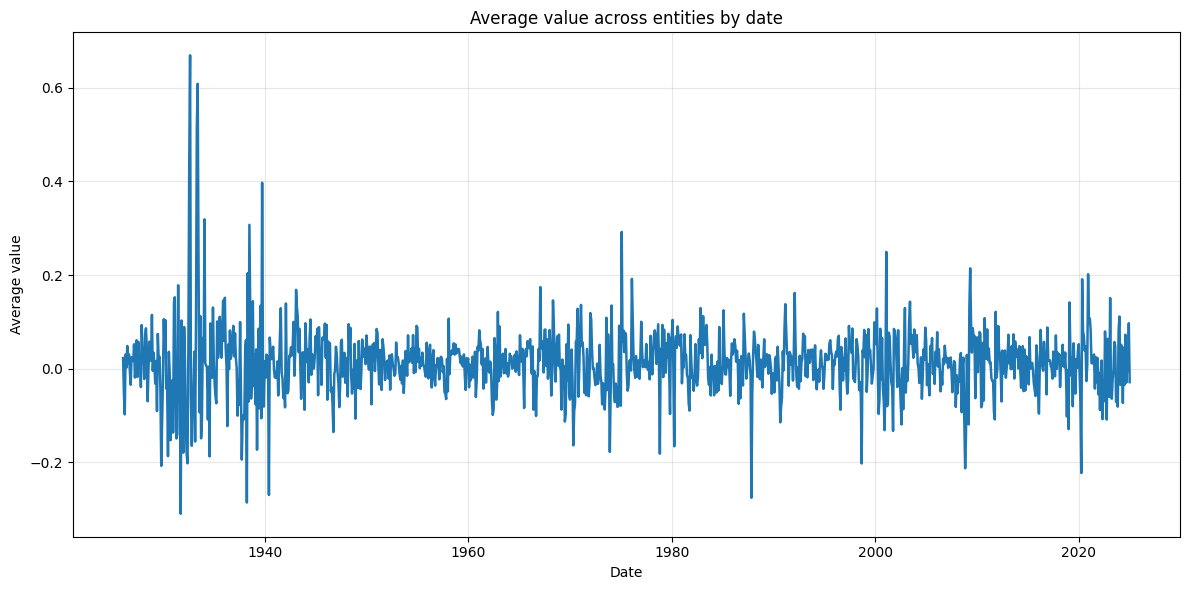
\includegraphics[width=.7\linewidth,height=200pt,width=400pt]{../docs_src/daily_avg_returns_CRSP_COMPU.png}
  \end{tabular}
  \caption{Average returns of all stocks for a given date}
  \label{fig:avg_returns_crsp}
\end{figure}

\begin{figure}[h!]
  \centering
  \begin{tabular}{@{}c@{}}
    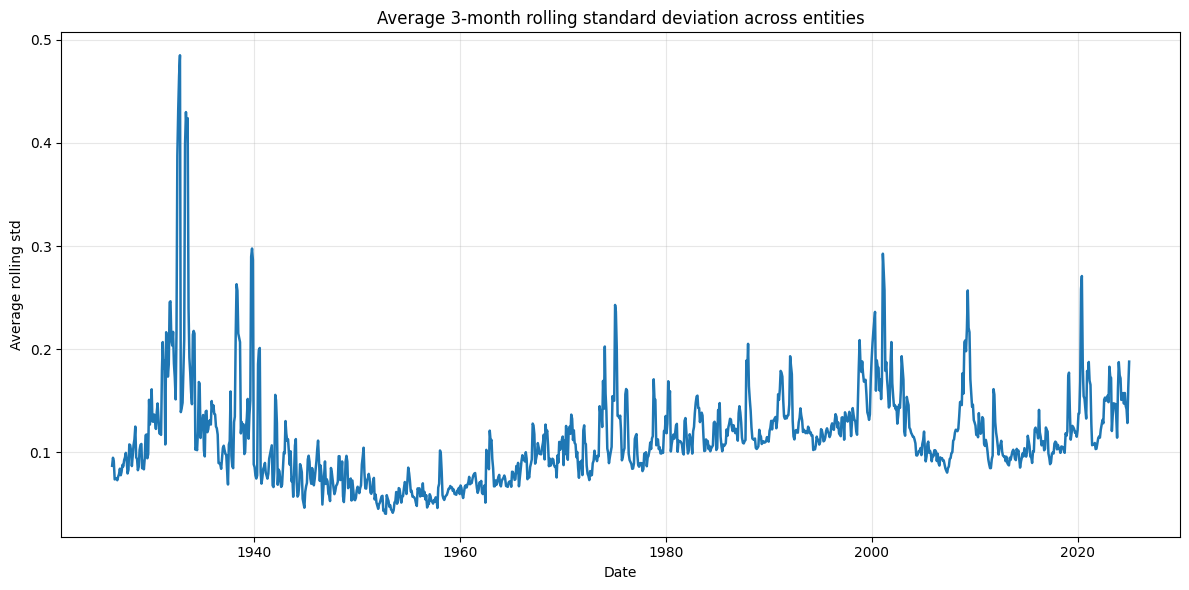
\includegraphics[width=.7\linewidth,height=200pt,width=400pt]{../docs_src/Average_three_month_rolling_std.png}
  \end{tabular}
  \caption{Average three month rolling standard deviation for a given date}
  \label{fig:avg_rolling_std_crsp}
\end{figure}


\subsubsection{US Treasuries}
\label{sec:treasuries}
% CRSP maturity-sorted portfolios Treasuries

The US Treasury dataset follows \cite{Gurkaynak2007}, whose methodology has become a common approach for constructing Treasury yield curves and returns. The results of using this methodology are published on the Federal Reserve Board's own website and underpins many studies in fixed income research.

Before estimating the yield curve, \citet{Gurkaynak2007} filter and clean the data in several steps. First, they restrict the sample to noncallable bonds and notes, excluding bills and other security types. Callable bonds embed optionality that contaminates pure interest rate risk measurement. For example, a bond trading at a premium with an embedded call option will exhibit negative convexity and compressed returns, distorting any analysis of term structure dynamics.

Second, the dataset focuses on bonds with remaining maturities between 0 and 5 years. This reflects market microstructure realities: bonds with longer maturities often suffer from illiquidity and fragmented trading, whereas the 0-5 year segment represents the most actively traded Treasury securities where price discovery is most efficient.

Third, the careful handling of accrued interest in return calculations is essential. Unlike equities, bond prices are quoted as clean prices (excluding accrued interest), but return calculations must incorporate coupon payments. Failing to account for this leads to dramatic miscalculations of returns, especially around coupon payment dates.

Fourth, a requirement for complete price and maturity information ensures that bonds with sporadic trading activity or ambiguous terms are excluded. This prevents noise from entering the yield curve estimation and return construction process.

Fifth, the use of month-end observations for portfolio aggregation avoids substantial day-of-month effects in Treasury markets. These effects arise from auction cycles, end-of-month portfolio rebalancing, and futures contract rolls, all of which can distort return measures if not properly controlled.

These filters, applied in the Gürkaynak, Sack, and Wright methodology, yield stable estimates that closely match dealer quotes and futures-implied yields. A comparison of the treasury bond returns dataset with the FTSFR dataset is shown in Figure \ref{fig:us_treasury_returns_comparison}.

\begin{figure}[h]
  \centering
  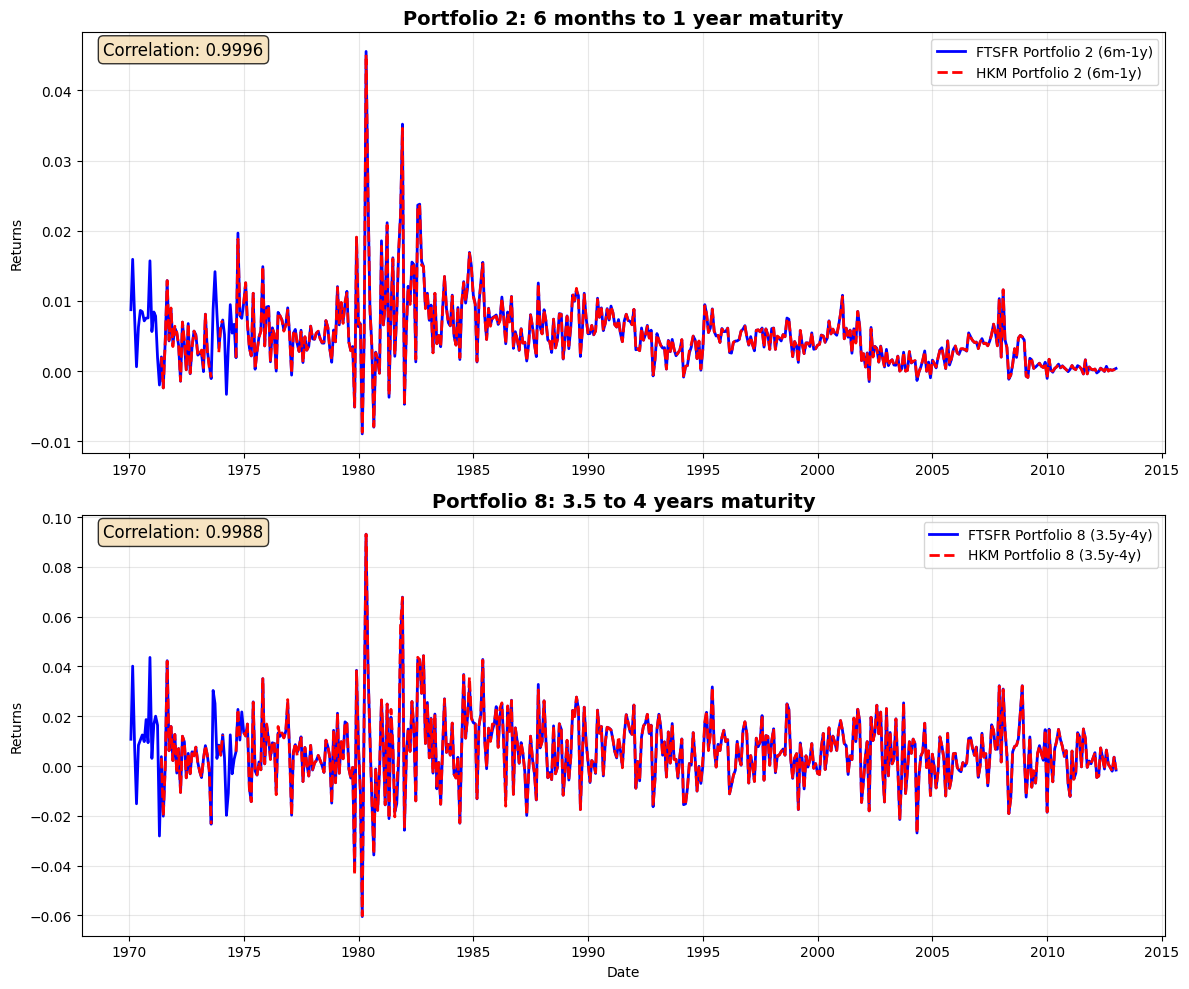
\includegraphics[width=0.8\textwidth]{../docs_src/us_treasury_compare.png}
  \caption{Comparison of He, Kelly, and Manela (2017) treasury bond returns dataset with FTSFR dataset}
  \label{fig:us_treasury_returns_comparison}
\end{figure}

\subsubsection{Corporate Bonds}
\label{sec:corporate_bonds}

% Nozawa (2017) yield-spread sorted portfolios
The corporate bond returns data is sourced from the TRACE (Trade Reporting and Compliance Engine) dataset, available at \url{openbondassetpricing.com}, and follows the methodology outlined in Nozawa (2017). This dataset incorporates several key elements to ensure accuracy and relevance. First, it includes market microstructure adjustments to correct for noise and enhance the reliability of bond prices and returns. It also applies stringent data filters, such as including only U.S.-domiciled firms and excluding private placements and convertible bonds. The dataset covers corporate bonds with sufficient outstanding amounts and complete information, and includes essential fields such as MMN-adjusted clean prices, amount outstanding, monthly returns, and credit spreads.

The cleaning and standardization procedure adheres to the rigorous framework established by Nozawa (2017) and adopted by He, Kelly, and Manela (HKM). In terms of bond selection, floating rate bonds and those with put or convertible features are excluded, although callable bonds are retained. Bonds are removed if their prices exceed matched Treasury prices or fall below \$0.01 per \$1 face value. For return processing, return reversals are eliminated if the product of adjacent returns is less than -0.04, and monthly returns are computed to avoid assumptions about reinvestment. In synthetic Treasury construction, Treasury bonds with identical cash flow structures are constructed for each corporate bond using Federal Reserve constant-maturity yield data. Excess returns and credit spreads are then calculated in price terms rather than yield spreads.

For portfolio construction, bonds are sorted into deciles based on credit spreads for each date. Value-weighted portfolio returns are computed using bond values-defined as the product of MMN-adjusted clean price and amount outstanding-as weights. To ensure data quality, defaults are verified using Moody's Default Risk Service, while CRSP and Compustat data supplement the equity and accounting information. Callable bonds are also incorporated into regression models using fixed effects.

The final output is a dataset containing monthly corporate bond portfolio returns sorted by credit spread deciles, making it well-suited for credit risk analysis and for benchmarking against other bond market data. The constructed returns are validated against the dataset by He, Kelly, and Manela (2017), which serves as a benchmark for credit spread deciles. As shown in Figure \ref{fig:corp_bond_returns_comparison}, the time series comparison between the two datasets exhibits strong alignment in return patterns, especially during volatile periods such as the 2008 financial crisis.

\begin{figure}[h!]
    \centering
    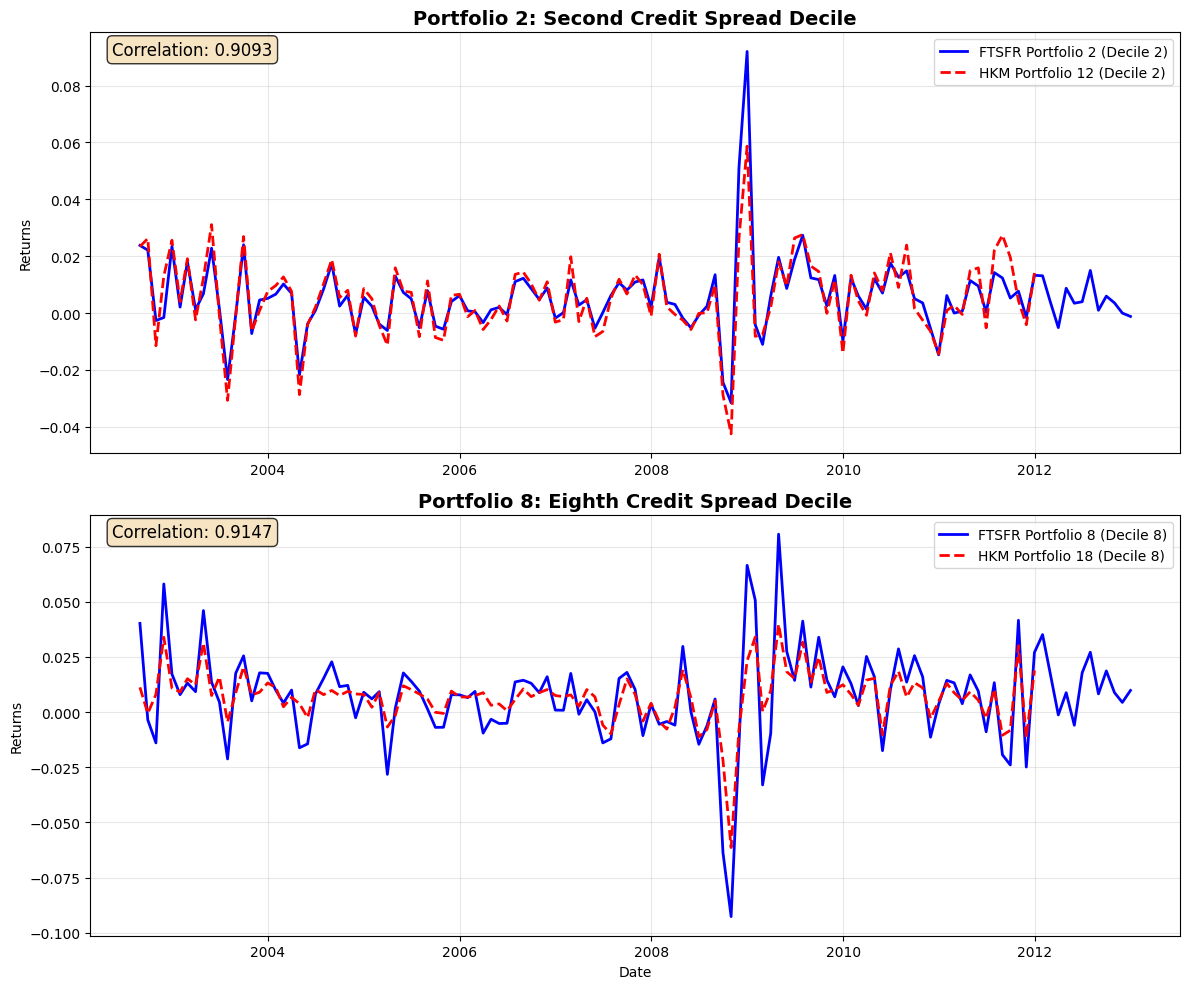
\includegraphics[width=0.8\textwidth]{../docs_src/corporate_returns_compare.png}
    \caption{Comparison of He, Kelly, and Manela (2017) corporate bond returns dataset with FTSFR dataset}
    \label{fig:corp_bond_returns_comparison}
  \end{figure}

% \subsubsection{Sovereign Bonds}
% \label{sec:sovereign}
% % Borri and Verdelhan (2012) portfolios

\subsubsection{Options}
\label{sec:options}
% Constantinides, Jackwerth and Savov (2013) S&P 500 portfolios

Our monthly SPX options portfolio returns series follows the data cleaning and portfolio construction methodology of \citet{Constantinides2013} (``CJS''), which has become the canonical approach for constructing option-based portfolios. This framework forms the foundation for numerous studies in derivatives pricing and risk management. \citet{He2017} (``HKM'') later adapted the CJS methodology to create a set of 18 option portfolios from the 54 portfolios in CJS. Our dataset includes both the original 54 CJS portfolios and the 18 HKM portfolios, for a total of 72 unique SPX option portfolios.

The original CJS paper used data from 1986 through 2012 (26 years of data). As of the time of writing, due to the unavailability of SPX option data from 1985 to 1995, we replicated the 54 CJS portfolios using data from January 1996 to December 2019 (23 years of data). As shown in Figure~\ref{fig:spx_options_over_time}, the number of SPX option observations has increased significantly over time, and since the volume of SPX options traded prior to 1996 was very low, we believe that our dataset from 1996 to 2019, while 3 years shorter is far richer in content and more relevant for current and future research.

The process to construct our returns series involved two major phases: (1) Replicating with the highest practical fidelity the raw daily data filtration and monthly portfolio construction procedures outlined in \citet{Constantinides2013}, and (2) Transforming these returns series into the 18 portfolios outlined in \citet{He2017}.

\paragraph{Options Data Series Access}

The final FTFSR data series comprise the monthly leverage-adjusted returns for call and put portfolios for both CJS 2013 (54 portfolios) and HKM 2017 (18 portfolios) for the period from Jan 1996--Dec 2019. Each portfolio is identified by a unique string of the form: 

\begin{center}
{\texttt{\{option type 'C' or 'P'\}\_\{moneyness $\times$ 1000\}\_\{maturity in days\}}}
\end{center}

Where ``C'' indicates a call option portfolio, ``P'' indicates a put option portfolio, ``moneyness'' is the strike price divided by the index price (e.g. 0.95, 1.00, 1.05), and ``maturity in days'' is the number of days to expiration (e.g. 30, 60, 90, 120, 150, 180). For example, the portfolio string ``C\_950\_30'' indicates a call option portfolio with moneyness of 0.95 and maturity of 30 days.



\paragraph{\textit{Phase 1a: Data Filtration in \citet{Constantinides2013}}}

In order to minimize possible quoting errors, CJS filtered the raw options data through three levels of filters. The filters are applied to the trade-in (buy) side to ensure the portfolios are buying into reliable quotes. When positions are exited, if there is no quote in the filtered data, the raw data is searched. These filters are detailed in \textit{Appendix B} of CJS.




\paragraph{\textit{Level 1 Filters}}
\begin{itemize}
  \item \textbf{Identical Filter:} Retain only one instance of quotes with the same \textit{option type}, \textit{strike price}, \textit{expiration date/maturity}, and \textit{price}.
  \item \textbf{Identical Except Price Filter:} For sets of quotes with identical terms (\textit{type}, \textit{strike}, and \textit{maturity}) but different prices, keep the quote whose \textit{T-bill-based implied volatility} is closest to that of its \textit{moneyness neighbors}, and delete the others.
  \item \textbf{Bid = 0 Filter:} Drop quotes with a \textit{bid price} of zero, thereby avoiding low-valued options. Also, a zero bid may indicate censoring as negative bids cannot be recorded.
  \item \textbf{Volume = 0 Filter:} Drop quotes with zero volume. Appendix B of CJS does not explicitly detail this filter, but we list it here for completeness since it is included in Table B.1 (Filters) of CJS. However, given that \textit{Appendix B} of \citet{Constantinides2013} did not describe this filter, we assume its inclusion in Table B.1 (Filter) of CJS was an error, and we have not implemented this filter in our replication.
\end{itemize}


\paragraph{\textit{Level 2 Filters}}
\begin{itemize}
  \item \textbf{Days to Maturity Filter:} Drop options with fewer than seven or more than 180 calendar days to expiration.
  \item \textbf{Implied Volatility Filter:} Remove all option quotes with implied volatilities lower than 5\% or higher than 100\%, computed using T-bill interest rates.
  \item \textbf{Moneyness Filter:} Remove all option quotes with moneyness (the ratio of strike price to index price) below 0.8 or above 1.2. These options have little value beyond their intrinsic value and are also very thinly traded.
  \item \textbf{Implied Interest Rate Filter:} Compute implied volatilities using T-bill interest rates from the Federal Reserve's H.15 release, assigning the closest available rate to each observation. Since T-bill rates may not be relevant for short maturities, we also compute a put-call parity-implied interest rate by imposing put-call parity on put-call pairs and adjusting the interest rate. We remove pairs with negative implied interest rates and assign the median-implied rate to all quotes of the same maturity and moneyness between 0.95 and 1.05, interpolating as needed.
  \item \textbf{Unable to Compute IV Filter:} Remove quotes that imply negative time value.
\end{itemize}

\paragraph{\textit{Level 3 Filters}}
\begin{itemize}
  \item \textbf{IV Filter:} The IV filter removes volatility outliers to reduce the prevalence of apparent butterfly arbitrage. This involves dropping calls and puts that have the same expiration date and strike price, but have anomalous prices due to extreme implied volatility values. For each date and maturity, we fit a quadratic curve to the implied volatility of puts and calls (separately) through the observed log implied volatilities.
  \item \textbf{Put-Call Parity Filter:} The puts and calls need to be matched up based on trading date, expiry date, and option type. We then calculate the put-call parity implied interest rate, and filter out outliers based on the standard deviation of the relative distance between the interest rate implied by put-call parity, and the calculated daily median 3-month T-bill rate from the pulled data.
\end{itemize}


\begin{figure}[H]
  \centering
  \begin{tabular}{@{}c@{}}
    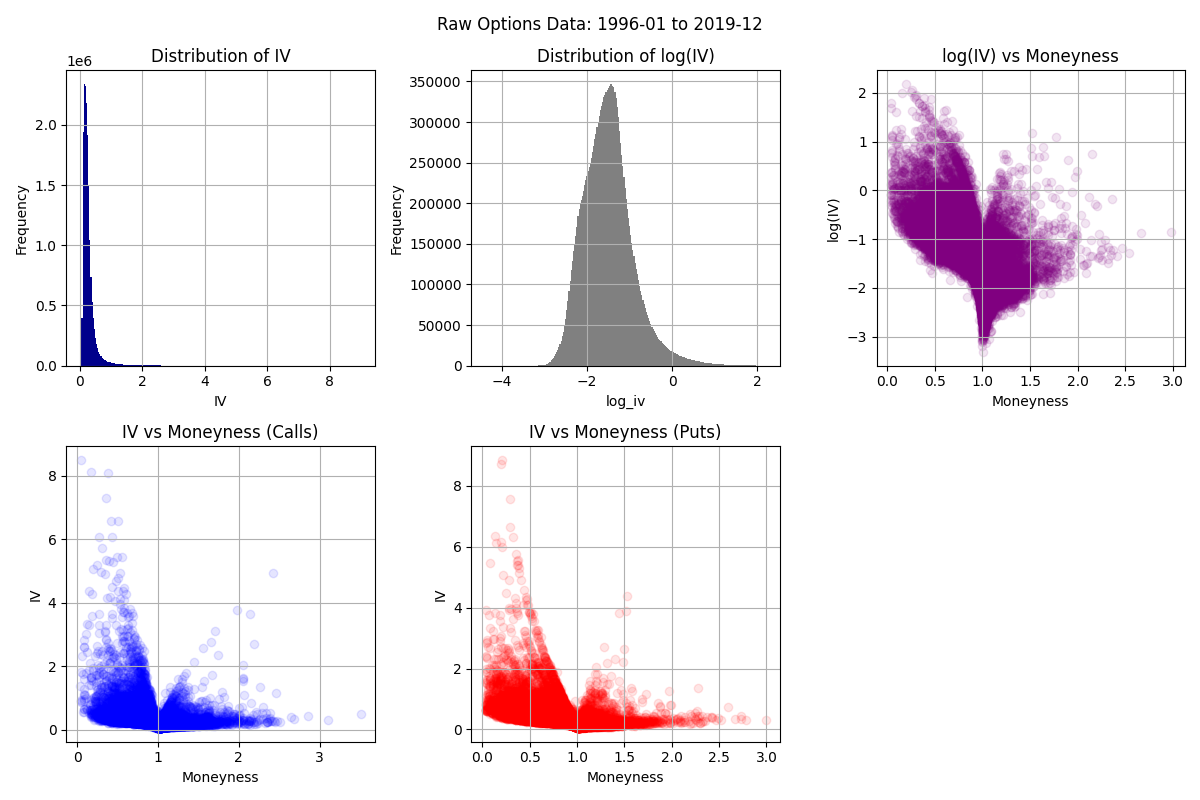
\includegraphics[width=\linewidth,height=0.666\linewidth]{../docs_src/RAW_1996-01_2019-12_iv.png}
  \end{tabular}
  \caption{Some visualizations of the raw SPX options data, prior to application of any filters. Each dot / point on these charts represents a single option in the raw data. Note that the time dimension is not shown, so this is a cross-sectional view of all options in the dataset.}
  \label{fig:raw_spx_options_data}
\end{figure}

\begin{figure}[H]
  \centering
  \begin{tabular}{@{}c@{}}
    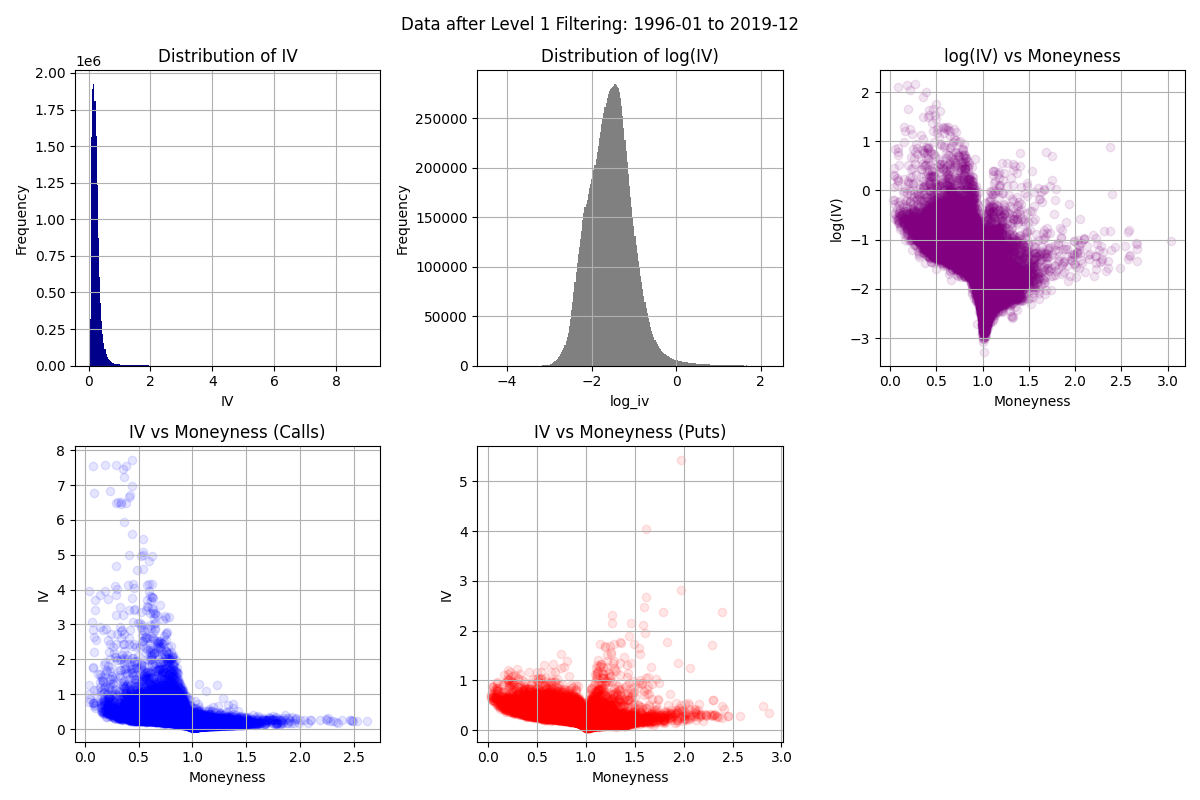
\includegraphics[width=\linewidth,height=0.666\linewidth]{../docs_src/L1_1996-01_2019-12_iv.png}
  \end{tabular}
  \caption{SPX options remaining after application of Level 1 filters. Notice reduction in outliers and cleaner distribution of volatility vs moneyness.}
  \label{fig:l1_spx_options_data}
\end{figure}


\begin{figure}[H]
  \centering
  \begin{tabular}{@{}c@{}}
    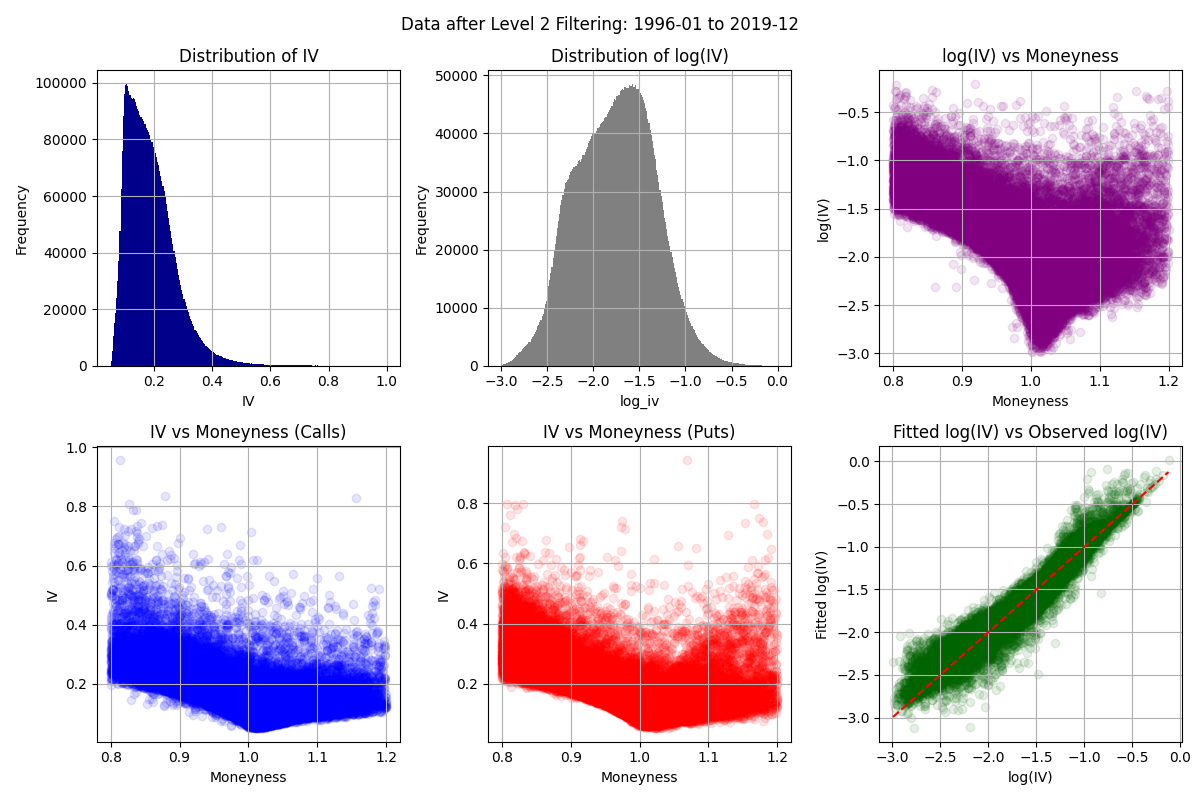
\includegraphics[width=\linewidth,height=0.666\linewidth]{../docs_src/L2_1996-01_2019-12_iv.png}
  \end{tabular}
  \caption{SPX options remaining after Level 2 filters.}
  \label{fig:l2_spx_options_data}
\end{figure}


\begin{figure}[H]
  \centering
  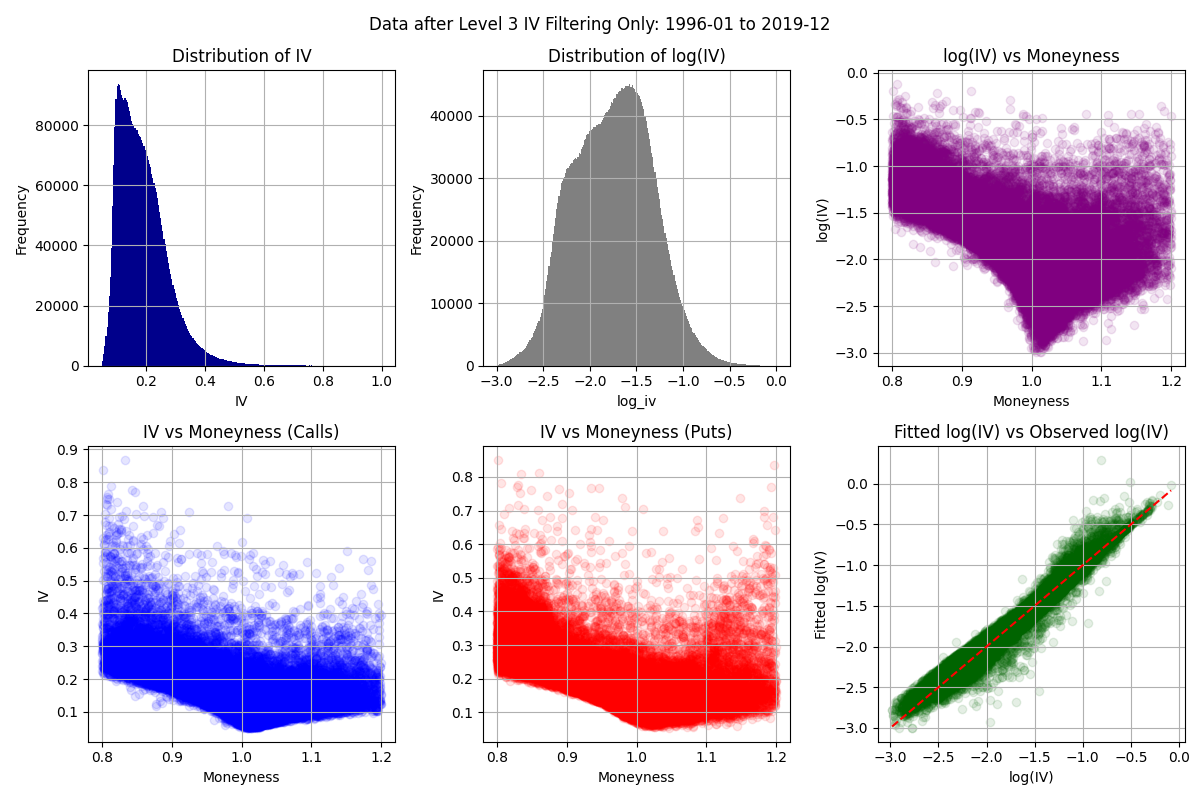
\includegraphics[width=\linewidth,height=0.666\linewidth]{../docs_src/L3_IV_1996-01_2019-12_iv.png}
  \caption{SPX options remaining after the Level 3 Implied Volatility filter (only).}
  \label{fig:l3_iv_only_spx_options_data}
\end{figure}


\begin{figure}[H]
  \centering
  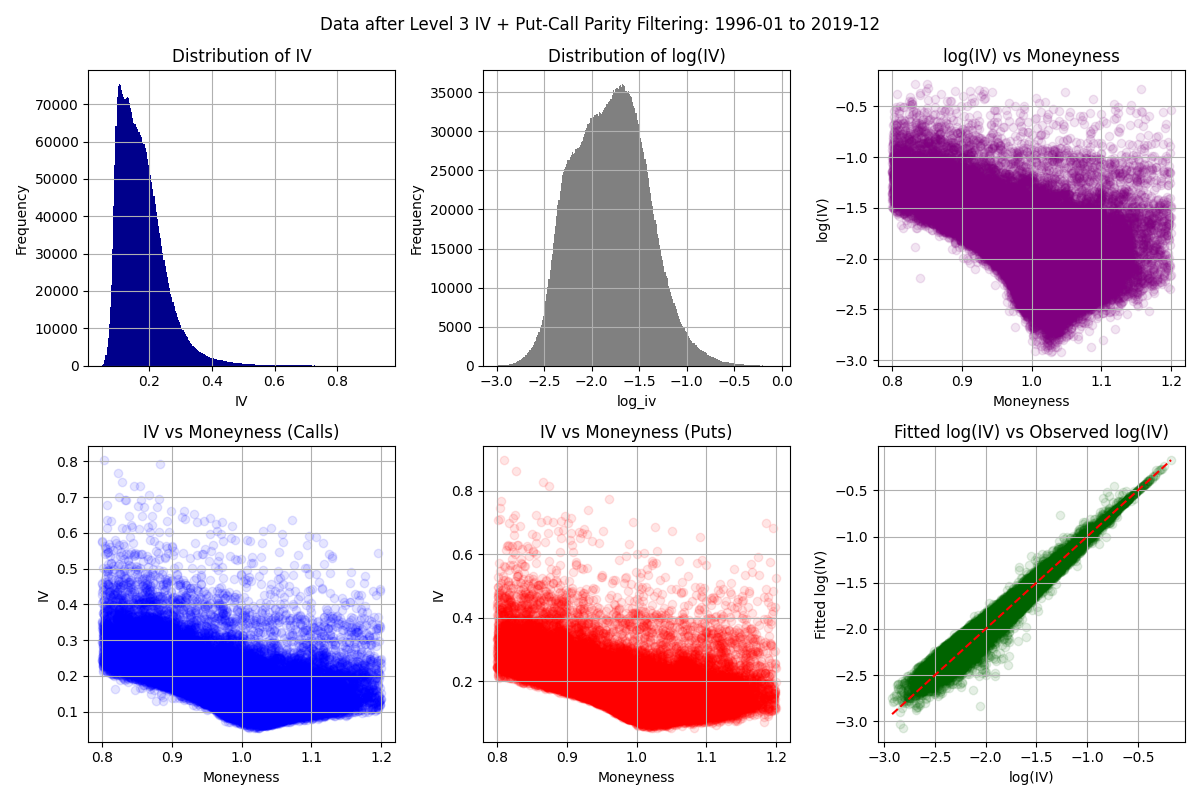
\includegraphics[width=\linewidth,height=0.666\linewidth]{../docs_src/L3_IV_PCP_1996-01_2019-12_iv.png}
  \caption{SPX options remaining after the Level 3 Implied Volatility and Put-Call Parity filters. Note how we observe the emergence of a volatility smile after the application of these filters.}
  \label{fig:l3_iv_pcp_spx_options_data}
\end{figure}


\paragraph{\textit{Phase 1b: Portfolio Construction in \citet{Constantinides2013}}}
\subsubsection*{Construction of Monthly Leverage-Adjusted Portfolio Returns in CJS}

\paragraph{Process}
The construction of the 27 call and 27 put portfolios in CJS is a multi-step process, with the objective of developing portfolio returns series that are stationary and only moderately skewed. The discrete bucketing of moneyness and days to maturity leads to multiple candidate options for each portfolio on each trading day. These options are given weights according to a bivariate Gaussian weighting kernel in moneyness and maturity (bandwidths: 0.0125 in moneyness and 10 days to maturity).

Each portfolio's daily returns are initially calculated as simple arithmetic returns, assuming the option is bought and sold at its bid-ask midpoint at each rebalancing. The one-day arithmetic return is then converted to a leverage-adjusted return. This procedure is achieved by calculating the one-day return of a hypothetical portfolio with $\omega_{BSM}^{-1}$ dollars invested in the option, and $(1 - \omega_{BSM}^{-1})$ dollars invested in the risk-free rate, where $\omega_{BSM}$ is the Black-Scholes-Merton elasticity based on the implied volatility of the option.

\begin{align}
\omega_{\text{BSM, Call}} &= \frac{\partial C_{\text{BSM}}}{\partial S} \cdot \frac{S}{C_{\text{BSM}}} > 1 \\
\omega_{\text{BSM, Put}}  &= \frac{\partial P_{\text{BSM}}}{\partial S} \cdot \frac{S}{P_{\text{BSM}}} < -1
\end{align}

Each leverage-adjusted call portfolio comprises a long position in a fraction of a call, and some investment in the risk-free rate.

Each leverage-adjusted put portfolio comprises a short position in a fraction of a put, and more than 100\% investment in the risk-free rate.

\paragraph{textit{Option Portfolio Construction Process}}


Below, we formalize the CJS portfolio construction process for a single trading day $t$ and a set of candidate call or put options. Each portfolio is defined by option type (call or put), target moneyness (specifically $0.90$, $0.925$, $0.95$, $0.975$, $1.00$, $1.025$, $1.05$, $1.075$, $1.10$), and target maturity (specifically $30$, $60$, or $90$ days). On any given day, available options rarely match the targets exactly; instead, multiple candidate options may be close in moneyness and maturity. Each candidate option has its own price and sensitivity to the underlying index. 

To aggregate these candidates, CJS applies a Gaussian kernel in moneyness and maturity, assigning weights to each option based on proximity to the targets. The kernel-weighted average price is used as the portfolio's option component. Portfolio returns are leverage-adjusted using Black-Scholes-Merton elasticity to standardize sensitivity across moneyness levels. 

The daily portfolio return from $t$ to $t+1$ is computed as the kernel-weighted average return of the candidate options, using weights from day $t$. This approach ensures that each portfolio reflects the closest available options to the target characteristics, with appropriate adjustment for leverage and sensitivity.

\subsubsection*{1. Gaussian Kernel Weighting}

Let:
\begin{itemize}
  \item $m_{i}$ = moneyness of option $i$
  \item $\tau_{i}$ = days to maturity of option $i$
  \item $k_{s}$ = target moneyness
  \item $\tau$ = target maturity
  \item $h_{m}$, $h_{\tau}$ = bandwidths for moneyness and maturity
  \item $d_{i}^2 = \left( \frac{m_{i} - k_{s}}{h_{m}} \right)^2 + \left( \frac{\tau_{i} - \tau}{h_{\tau}} \right)^2$
\end{itemize}

Then the unnormalized Gaussian weight for option $i$ is:
\[
w_{i}^* = \exp\left( -\frac{1}{2} d_{i}^2 \right)
\]

The normalized kernel weight:
\[
w_{i} = \frac{w_{i}^*}{\sum_j w_j^*}
\]

\subsubsection*{2. Option Elasticity}

Let:
\begin{itemize}
  \item $S_{t}$ = underlying index level at time $t$
  \item $P_{i}$ = price of option $i$
  \item $\Delta_{i}$ = option delta
\end{itemize}

Then:
\[
\varepsilon_{i} = \frac{S_t \cdot \Delta_{i}}{P_{i}}
\]

\subsubsection*{3. Arithmetic Return of Option $i$}

Let:
\begin{itemize}
  \item $P_{i,t-1}$ = price of option $i$ at time $t-1$
  \item $P_{i,t}$ = price of option $i$ at time $t$
\end{itemize}

Then:
\[
r_{i} = \frac{P_{i,t} - P_{i,t-1}}{P_{i,t-1}}
\]

\subsubsection*{4. Leverage-Adjusted Portfolio Construction}

Let:
\begin{itemize}
  \item $r_{f}$ = risk-free rate on day $t$
\end{itemize}

The leverage-adjusted return of the call portfolio is:
\[
R_t^{call} = \sum_{i} w_{i} \cdot \frac{1}{\varepsilon_{i}} \cdot r_{i} + \left(1 - \sum_{i} w_{i} \cdot \frac{1}{\varepsilon_{i}} \right) \cdot r_f
\]

The leverage-adjusted return of the put portfolio is:
\[
R_t^{put} = -\sum_{i} w_{i} \cdot \frac{1}{\varepsilon_{i}} \cdot r_{i} + \left(1 + \sum_{i} w_{i} \cdot \frac{1}{\varepsilon_{i}} \right) \cdot r_f
\]



\subsubsection*{5. Handling Missing Data (NaN Filling)}

CJS implement a multi-step process to address options with missing prices, as detailed in Section 1.3 ``Portfolio Formation'' of their paper. We reserve the implementation of this NaN-filling procedure for a future version of this dataset. For the current version, we compound the daily portfolio returns into monthly returns, which matches the final form of the data utilized in the paper.


\paragraph{\textit{Phase 2: Returns Series Transformation in \citet{He2017}}}
\subsubsection*{Construction of 18 Portfolio Return Series in HKM}

\citet{He2017} reduce the 54 portfolios constructed in \citet{Constantinides2013} to 18 portfolios by taking an equal-weight average across the three maturities (30, 60, 90 days) for all CJS portfolios with the same moneyness. We implement that procedure to obtain the final return series for the FTSFR.

Let \( R_{m,j,t} \) be the return for moneyness \( m \), maturity \( j \), at time \( t \).
The HKM portfolio return for moneyness \( m \) at time \( t \) is:
\[
R_{m,t}^{\mathrm{HKM}} = \frac{1}{3} \sum_{j=1}^{3} R_{m,j,t}
\]
For each moneyness group, the HKM portfolio return is the simple average of the three corresponding CJS portfolio returns (one for each maturity) at each time point.

This averaging is done separately for calls and puts, resulting in 9 call portfolios and 9 put portfolios (total 18 portfolios).



\subsubsection*{Portfolio Returns Analysis}

The objective of the data filtration process was to construct portfolios whose returns are approximately normal and only moderately skewed. We analyzed the distributional properties of the 54 CJS portfolios and the 18 HKM portfolios using standard statistical tests and summary statistics.

\paragraph{Statistical Normality Tests}
To assess the normality of portfolio returns, we applied several standard tests:
\begin{itemize}
  \item \textbf{Shapiro-Wilk Test:} Tests the null hypothesis that the data are drawn from a normal distribution. The test statistic is
  \[
  W = \frac{\left( \sum_{i=1}^n a_i x_{(i)} \right)^2}{\sum_{i=1}^n (x_i - \bar{x})^2}
  \]
  where $x_{(i)}$ are ordered sample values and $a_i$ are constants.
  \item \textbf{Jarque-Bera Test:} Tests whether sample skewness and kurtosis match a normal distribution. The test statistic is
  \[
  JB = \frac{n}{6} \left( S^2 + \frac{(K-3)^2}{4} \right)
  \]
  where $S$ is sample skewness and $K$ is sample kurtosis.
  \item \textbf{D'Agostino and Pearson's Normality Test (Normaltest):} Combines skewness and kurtosis to test for normality.
\end{itemize}
Low $p$-values (typically $<0.05$) indicate rejection of normality.

\paragraph{Summary Statistics}
Table~\ref{tab:portfolio_stats} presents descriptive statistics for the returns of the CJS and HKM portfolios. The statistics include count, mean, standard deviation, minimum, 25th percentile, median, 75th percentile, and maximum, following the convention of \texttt{pd.DataFrame.describe()}.

\begin{table}[H]
  \centering
  \caption{Descriptive Statistics of Portfolio Returns}
  \label{tab:portfolio_stats}
  \begin{tabular}{lcc}
    \toprule
    \textbf{Statistic} & \textbf{CJS Portfolios} & \textbf{HKM Portfolios} \\
    \midrule
    Count   & 54                          & 18                          \\
    Mean    & 1.64 (skew), 14.5 (kurtosis)  & 1.87 (skew), 16.8 (kurtosis) \\
    Std     & 2.26 (skew), 23.8 (kurtosis)  & 2.64 (skew), 30.3 (kurtosis) \\
    Min     & -0.91 (skew), 0.7 (kurtosis)  & -0.91 (skew), 0.7 (kurtosis) \\
    25\%    & 0.12 (skew), 2.1 (kurtosis)   & 0.12 (skew), 2.1 (kurtosis) \\
    \rowcolor{blue!20}
    Median  & 0.77 (skew), 4.6 (kurtosis)   & 0.78 (skew), 3.1 (kurtosis) \\
    75\%    & 2.41 (skew), 12.3 (kurtosis)  & 2.41 (skew), 12.3 (kurtosis) \\
    Max     & 11.1 (skew), 152.7 (kurtosis) & 9.8 (skew), 129.3 (kurtosis) \\
    \bottomrule
  \end{tabular}
\end{table}

\textbf{Note:} We did not implement the NaN-filling logic described in the original CJS paper. As a result, missing data may affect the distributional properties of the portfolio returns, and these results and conclusions may change in future versions once NaN handling is incorporated.

\paragraph{Results for CJS Portfolios}

Nearly all CJS portfolios reject normality based on the Shapiro-Wilk, Jarque-Bera, and Normaltest $p$-values, which are close to zero. The mean skewness is 1.64 and the median is 0.77, indicating distributions are generally right-skewed with long right tails. The mean kurtosis is 14.5 and the median is 4.6, suggesting many portfolios are leptokurtic (fat-tailed), with some experiencing rare but large return shocks. However, the median skewness and kurtosis are much closer to the normal values (skewness $=0$, kurtosis $=3$), implying that most portfolios are only moderately skewed and not excessively heavy-tailed. These results confirm that the filtration and leverage-adjustment procedures substantially mitigate extreme non-normality, achieving the authors' objective of constructing portfolios with returns that are approximately normal and only moderately skewed.

\paragraph{Results for HKM Portfolios}
Most HKM portfolios also reject normality, although a few have higher $p$-values and may plausibly be normal. The mean skewness is 1.87 and the median is 0.78, again showing generally positive skewness. The mean kurtosis is 16.8 and the median is 3.1, which is very close to the normal value of 3. This suggests that, while some portfolios have extreme outliers, the median HKM portfolio is only moderately skewed and has kurtosis similar to a normal distribution. These findings further validate that the aggregation and transformation steps in HKM produce portfolio returns with moderate skewness and near-normal kurtosis.

\paragraph{Overall Findings}
In summary, the data filtration and portfolio construction procedures yield return series that are not perfectly normal, but the median portfolio for both CJS and HKM is much closer to normal and only moderately skewed. This demonstrates that the authors' objectives were largely met: the median portfolio is well-suited for empirical asset pricing tests that assume approximate normality, even though some portfolios remain highly non-normal due to outliers. The successful replication of these distributional properties confirms the effectiveness of the canonical cleaning and construction methods.



\subsubsection{Foreign Exchange}
\label{sec:fx}
% Lettau et al. (2014) and Menkhoff et al. (2012)
The Foreign Currencies returns series we generated uses spot rate changes and local repo rates to generate a USD-based
foreign currency returns. 

We are replicating a process where we convert our USD into the foreign currency $i$ at end of day $t - 1$, 
invest it in the repo market, then switch the currency back to USD on day $t$. 

\begin{equation}
  ret_{t, i} \;=\; \frac{spot_{t - 1, i}}{spot_{t, i}} \times fret_{t, i}
\end{equation}

where
\begin{itemize}
 \item $i$ is the foreign currency
 \item $t$ is the date of the implied foreign currency return
 \item $ret$ is the return of USD invested in the foreign currency
 \item $fret$ is the return of the foreign currency when invested in their overnight repo market
 \item $spot$ is the spot price of the currency (how much 1 USD is worth in the foreign currency)
\end{itemize}

\begin{figure}
  \centering
  \begin{tabular}{@{}c@{}}
    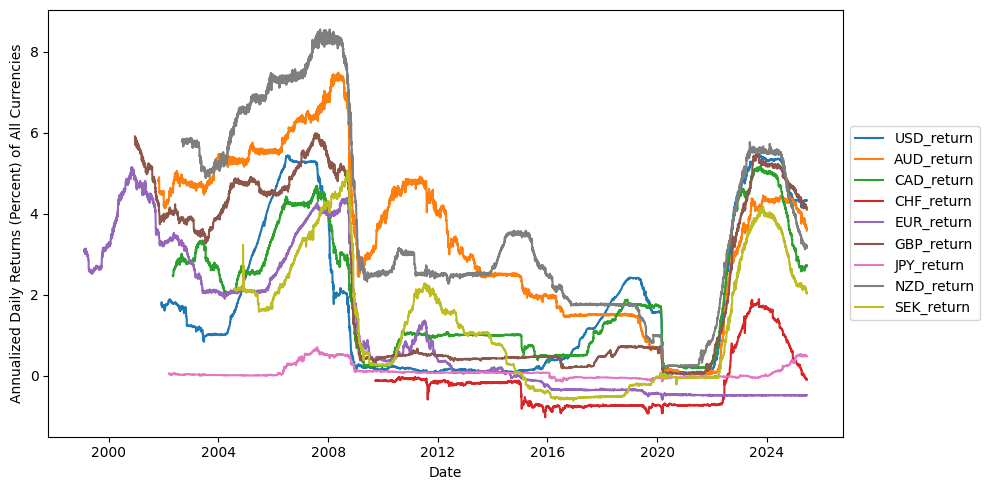
\includegraphics[width=.7\linewidth,height=200pt,width=400pt]{../docs_src/FX_returns.png} \\[\abovecaptionskip]
  \end{tabular}

  \caption{Foreign Currency Returns}
  \label{fig:fx_returns}
\end{figure}

\FloatBarrier

\subsubsection{Commodities}
\label{sec:commodities}
% Yang (2013) methodology
The commodity dataset follows \cite{Yang2013}, but in practice we adopt the 
implementation of \cite{Koijen2018}, who provide Bloomberg tickers for the 
Goldman Sachs Commodity Index (GSCI). These GSCI indices have become the 
standard source for replication in commodity asset pricing, as they embed the 
official methodology for contract selection, roll schedules, and weighting 
across major futures markets. By relying on these pre-constructed Bloomberg 
series, we avoid the pitfalls of ad hoc roll choices or inconsistent maturity 
definitions that can bias commodity return factors.

Our processing of the GSCI data proceeds in several steps. First, we retrieve the 
designated Bloomberg excess return indices via the \texttt{xbbg} interface and 
store them as standardized parquet files. Second, we align all series to a 
monthly frequency by selecting the last observation in each calendar month and 
computing simple percentage returns. Third, we harmonize naming conventions and 
drop missing values, ensuring that each commodity return series is complete and 
comparable across the sample period. Finally, we compare these series
with those published by \cite{He2017}. He, Kelly, and Manela (HKM) publish returns series for 23 commodities from a broader pool of 31 commodities, but do not provide the names of the commodities nor the exact pool of commodities they used. To identify the commodities in their dataset, we computed the pairwise correlations between our Bloomberg GSCI-based returns and the corresponding series in \cite{He2017}. We then used the linear assignment algorithm to find the optimal one-to-one commodity matches, maximizing the total correlation between the two datasets.

The following figures illustrate the outcome of this replication exercise. 
Figure~\ref{fig:commod_return_comparison} reports the pairwise correlations between our 
Bloomberg GSCI-based returns and the corresponding series in \cite{He2017}. 
While many commodities show very high alignment, several pairs exhibit unusually 
low correlations. We interpret these discrepancies as arising from ticker 
mismatches and differences in the underyling datasets used: the lists provided by \cite{Koijen2018} and \cite{Yang2013} do not 
perfectly overlap, and it is unclear which exact subset was ultimately adopted 
in \cite{He2017}. Furthermore, \cite{He2017} uses a different datasource than
Bloomberg, which we use.
In other words, low-correlation pairs likely reflect incorrect 
matches rather than genuine return differences. The accompanying heatmap in 
Figure~\ref{fig:commod_heatmap} highlights this heterogeneity visually, with 
clusters of high-correlation matches alongside a handful of clear mismatches.

\begin{figure}[H]
  \centering
  \begin{tabular}{@{}c@{}}
    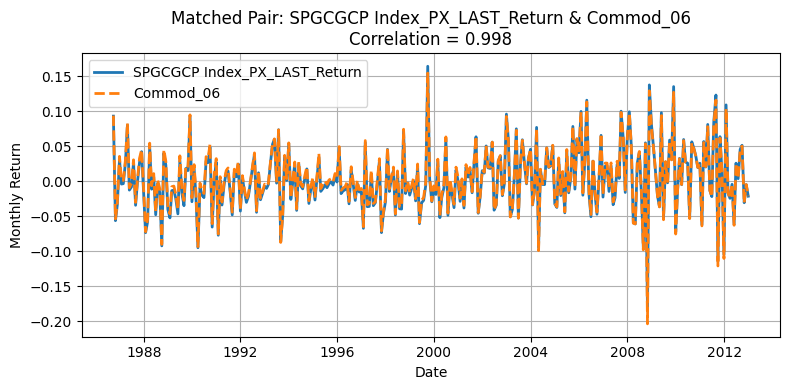
\includegraphics[width=\linewidth]{../docs_src/commod_return_comparison.png} \\[\abovecaptionskip]
  \end{tabular}
  \caption{Pairwise Correlations between GSCI Commodity Returns and Yang (2013) Commodity Returns}
  \label{fig:commod_return_comparison}
\end{figure}

\begin{figure}[H]
  \centering
  \begin{tabular}{@{}c@{}}
    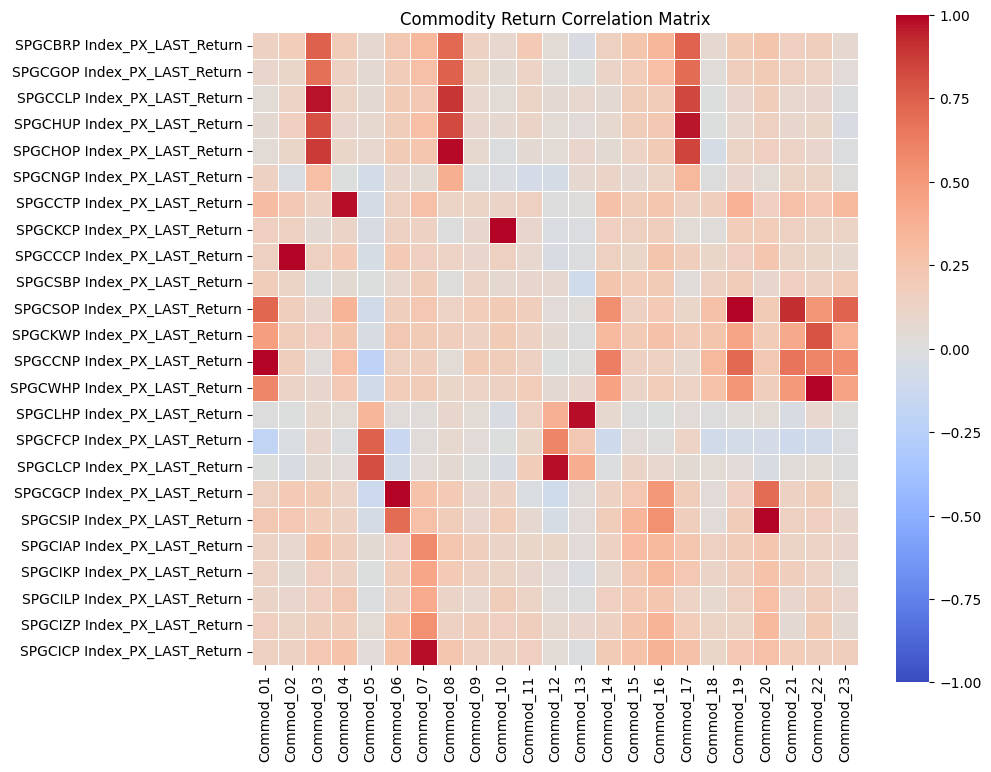
\includegraphics[width=\linewidth]{../docs_src/commod_heatmap.png} \\[\abovecaptionskip]
  \end{tabular}
  \caption{Heatmap of Pairwise Correlations between GSCI Commodity Returns and Yang (2013) Commodity Returns}
  \label{fig:commod_heatmap}
\end{figure}


\subsubsection{Credit Default Swaps}
\label{sec:cds}
% Markit data following Palhares (2013)

[Asset class content to be filled in...]

\subsection{Arbitrage Spread Datasets}
\label{sec:arbitrage}

% TODO: Document each arbitrage spread construction
% For EACH arbitrage spread:
% - Explain the economic intuition behind the trade
% - Detail the exact construction methodology
% - Show replication of statistics from Siriwardane et al.
% - Discuss what violations of these spreads tell us about market segmentation

Following \cite{Siriwardane2021}, we construct various arbitrage spreads that measure market segmentation.

\subsubsection{Covered Interest Parity (CIP)}
% Construction using spot, forward FX and interest rates
     

During periods of market stress, such as the 2008 financial crisis and the 2020 COVID-19
pandemic, covered interest parity (CIP) may no longer hold as the forward---spot differential 
no longer exactly offsets interest-rate differentials. Factors contributing to this phenomenon include:
Heightened Counterparty-Credit Risk, Liquidity Constraints, or Regulatory Pressures.

In other periods, deviations from CIP typically stem from market inefficiencies and are 
small in magnitude and are short-lived in timeframe due to arbitrage activities.

Our analysis examines CIP deviations across eight G10 currencies against the USD, 
using data from 1999 onwards sourced through Bloomberg Terminal.

\paragraph{The dataset includes:}
\begin{itemize}
    \item Spot exchange rates for each currency pair
    \item 3-month forward points for each currency pair
    \item 3-month Overnight Index Swap (OIS) rates for each currency
\end{itemize}

\paragraph{Data Standardization:}
\begin{itemize}
    \item Forward points are scaled appropriately (per 10,000 for most currencies, per 100 for JPY)
    \item Currencies conventionally quoted as USD-per-foreign-currency (EUR, GBP, AUD, NZD) are converted to reciprocal rates for consistency
    \item OIS rates serve as our risk-free benchmark to align with other arbitrage spread studies
\end{itemize}

We successfully replicate the CIP spreads as calculated by Siriwardane et al. (2023),
as seen in 
% this side by side comparison of 
our calculated currency respective
arbitrage spreads versus those reported in their paper. If you compare
the spreads in Figure \ref{fig:cip_comparison}, you will see that they are nearly identical
to those reported in their paper.

\begin{figure}
  \centering
%   \begin{tabular}{@{}c@{}}
%     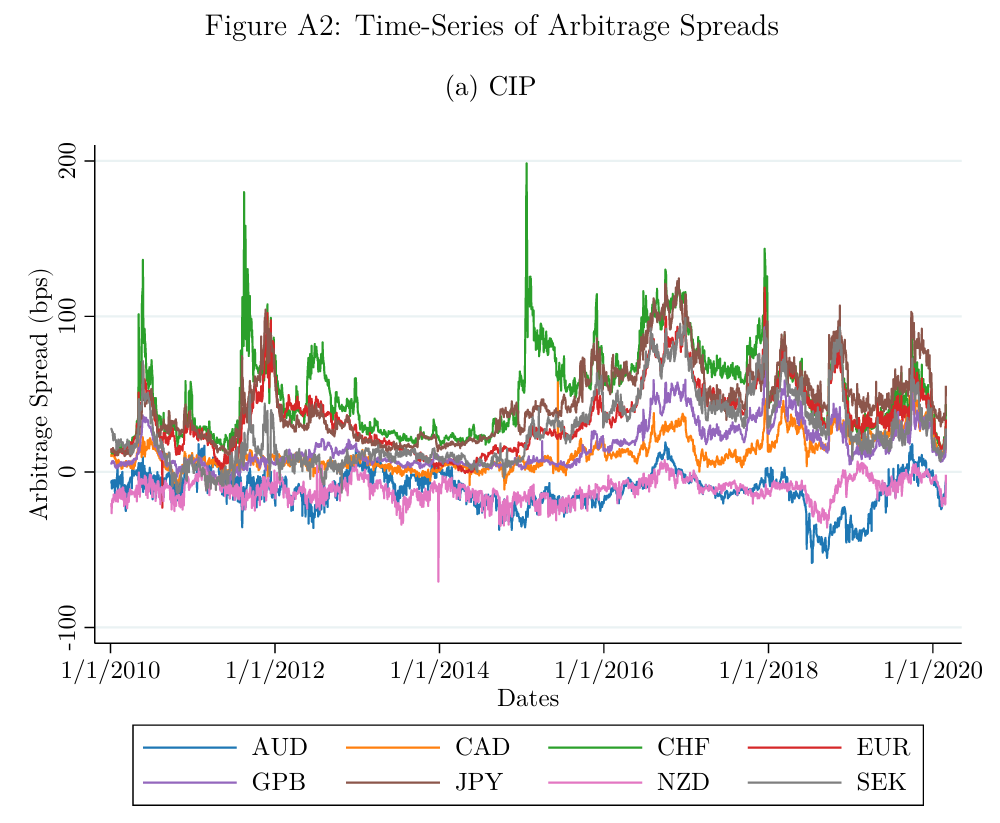
\includegraphics[width=.7\linewidth]{../docs_src/SegArb_CIP_Timeseries.png} \\[\abovecaptionskip]
%     \small (a) Findings in Siriwardane et al. (2023)
%   \end{tabular}

%   \vspace{\floatsep}

  \begin{tabular}{@{}c@{}}
    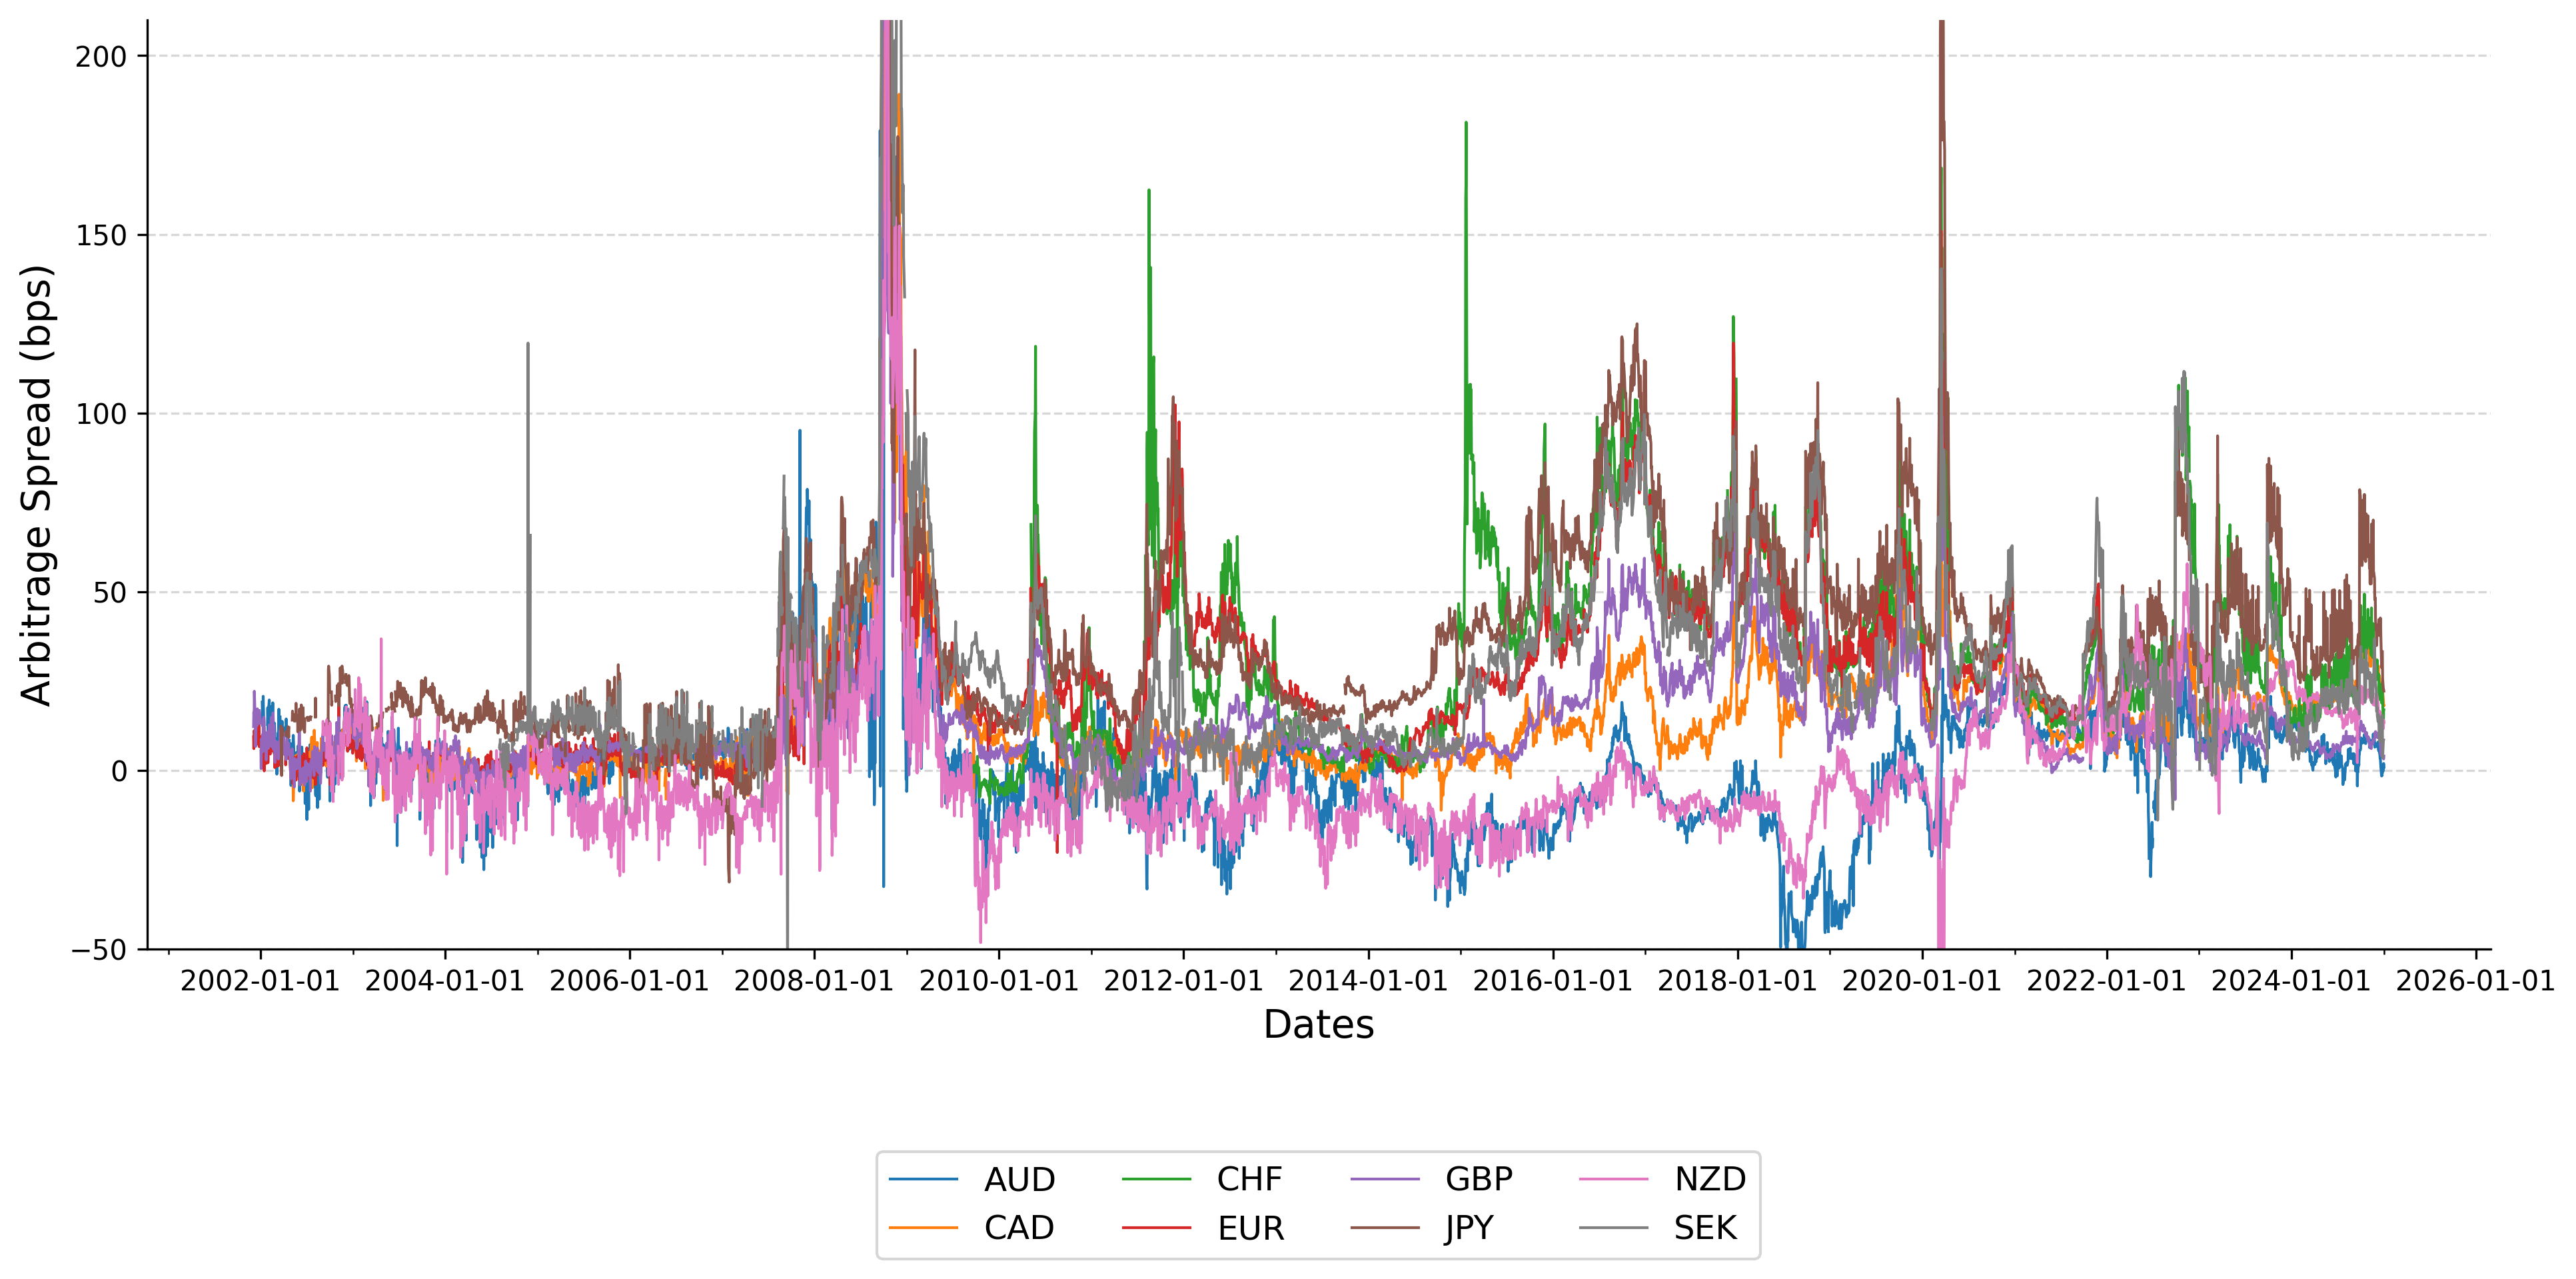
\includegraphics[width=.99\linewidth]{../docs_src/CIP_replicate.png} 
  \end{tabular}

  \caption{Comparison of CIP Arbitrage spreads}
  \label{fig:cip_comparison}
\end{figure}

\FloatBarrier


During the overlapping periods of both datasets, the CIP spreads are nearly identical.
Our findings confirm the presence of CIP deviations, particularly during periods of
market stress, consistent with the conclusions drawn by Siriwardane et al. (2023).


\subsubsection{Treasury Spot-Futures Basis}
% Government bond basis trades

\subsubsection{Treasury-Swap Spread}
% Treasury vs interest rate swap arbitrage

\subsubsection{TIPS-Treasury Spread}
% Inflation-linked vs nominal bond spreads

\subsubsection{CDS-Bond Basis}
% Credit default swap vs cash bond arbitrage

Credit Default Swaps (CDS) are "insurance contracts" against the default of underlying
corporate debt. The buyer of CDS protection pays a the CDS spread as a 
fixed annuity premium to the seller for a horizon $\tau$. If there is a default
before the time horizon $\tau$, the buyer receives the difference between
the bond's par value and its market value from the seller. 
As a result, the payoff of this portfolio should not deviate from the risk free bond. 
The resulting difference between CDS spread and floating rate spread (corporate bond rate - risk free rate)
is defined by the authors as the CDS-basis.

The authors define the CDS basis (CB) as

\begin{equation}
  CB_{i,t,\tau} \;=\; CDS_{i,t,\tau} \;-\; FR_{i,t,\tau},
\end{equation}

where:
\begin{itemize}
  \item $FR_{i,t,\tau}$ = time $t$ floating-rate spread implied by a fixed-rate corporate bond issued by firm $i$ at tenor $\tau$,
  \item $CDS_{i,t,\tau}$ = time $t$ Credit Default Swap (CDS) par spread for firm $i$ with tenor $\tau$.
\end{itemize}

A negative basis implies an investor could earn a positive arbitrage profit by going long the bond and purchasing CDS protection. 
The investor would pay a lower par spread than the coupon of the bond itself and then receive value from the default.

The value of $FR$ is substituted by the paper with Z-spread which we also modify in our construction. We address the substitution in detail later.

The value of CDS par spread is interpolated by the authors using a cubic spline function as
not all necessary tenors are present.

Given the CDS spread from above, traditional construction of a risk-free rate for implied arbitrage implies the following return:

\begin{equation}
  rfr^{CDS}_{i,t,\tau} \;=\; y_{t,\tau} \;-\; CB_{i,t,\tau},
\end{equation}

where:
\begin{itemize}
  \item $y_{t,\tau}$ = maturity-matched Treasury yield at time $t$.
\end{itemize}

The implied risk-free arbitrage is then defined as the treasury yield in addition to the basis received when executing the CDS basis trade (investor benefits from negative basis).

The CDS-Bond basis is plotted in Figure \ref{fig:cds_replicate}.    

\subsubsection{Z-Spread (Zero-Volatility Spread)}

\paragraph*{Mathematical definition}
For a bond with cash-flows $CF_t$ at times $t=1,\dots,N$ and Treasury spot rates $s_t$,
\begin{equation*}
P = \sum_{t=1}^{N} \frac{CF_t}{\bigl(1+s_t+Z\bigr)^t}.
\end{equation*}
The constant $Z$ that solves this equation is the \textbf{Z-spread}.

\paragraph*{Intuition}
$Z$ is the uniform extra yield added to every point on the risk-free spot curve so that the discounted cash-flows equal the bond's dirty price $P$. It compensates investors for credit and liquidity risk relative to Treasuries.

\paragraph*{Link to Yield-to-Maturity}
Setting the Z-spread pricing equation equal to the standard YTM equation gives
\begin{equation}
\label{eq:ytm_z_spread}
\sum_{t=1}^{N}\frac{CF_t}{(1+y)^t}
=\sum_{t=1}^{N}\frac{CF_t}{\bigl(1+s_t+Z\bigr)^t}
\end{equation}
where $y$ is the bond's yield-to-maturity. Except for the trivial flat-curve case ($s_t=s$), equation (\ref{eq:ytm_z_spread}) has no algebraic solution-$y$ or $Z$ must be found numerically.

\paragraph*{Continuous-Compounding Identity}
Rewrite discounts as $e^{-r t}$. With PV-weights
\begin{equation*}
w_t=\frac{CF_t\,e^{-(s_t+Z)t}}{P},\qquad\sum_{t}w_t=1,
\end{equation*}
equation (\ref{eq:ytm_z_spread}) yields the convenient mean-value relationship
\begin{equation}
y \;=\; \sum_{t=1}^{N} w_t\,(s_t+Z)\tag{A2}
\end{equation}
Thus YTM is the PV-weighted average of the spot rates plus the Z-spread.

\paragraph*{Practical Proxy: YTM Credit Spread}
Analysts often approximate $Z$ with the \textbf{credit spread}
\begin{equation*}
\Delta y = y_{\text{bond}} - y_{\text{Treasury-DM}},
\end{equation*}
where $y_{\text{Treasury-DM}}$ is the yield on a Treasury portfolio matched to the bond's (modified) duration.

\paragraph*{Why it works}
\begin{enumerate}
    \item A small parallel shift $Z$ applied to all discount rates changes price by $-D_{\text{mod}}\;Z$. For modest spreads, this produces nearly the same price change as replacing the spot curve with a single rate shift $\Delta y$.
    \item Duration-matching the Treasury benchmark neutralises curve-shape effects, so $\Delta y$ isolates the average extra yield attributable to credit/liquidity risk.
    \item Empirically, $\Delta y$ tracks $Z$ closely for plain-vanilla, option-free bonds, making it a ``good-enough'' proxy when full spot-curve data or iterative Z-spread calculations are impractical.
\end{enumerate}

\paragraph*{Note}
Z-spread is said to be populated by Markit in the CDS dataset but during the reconstruction process we found no proxy. Thus, we chose our own construction.

% \begin{figure}
%   \centering
%   \begin{tabular}{@{}c@{}}
%     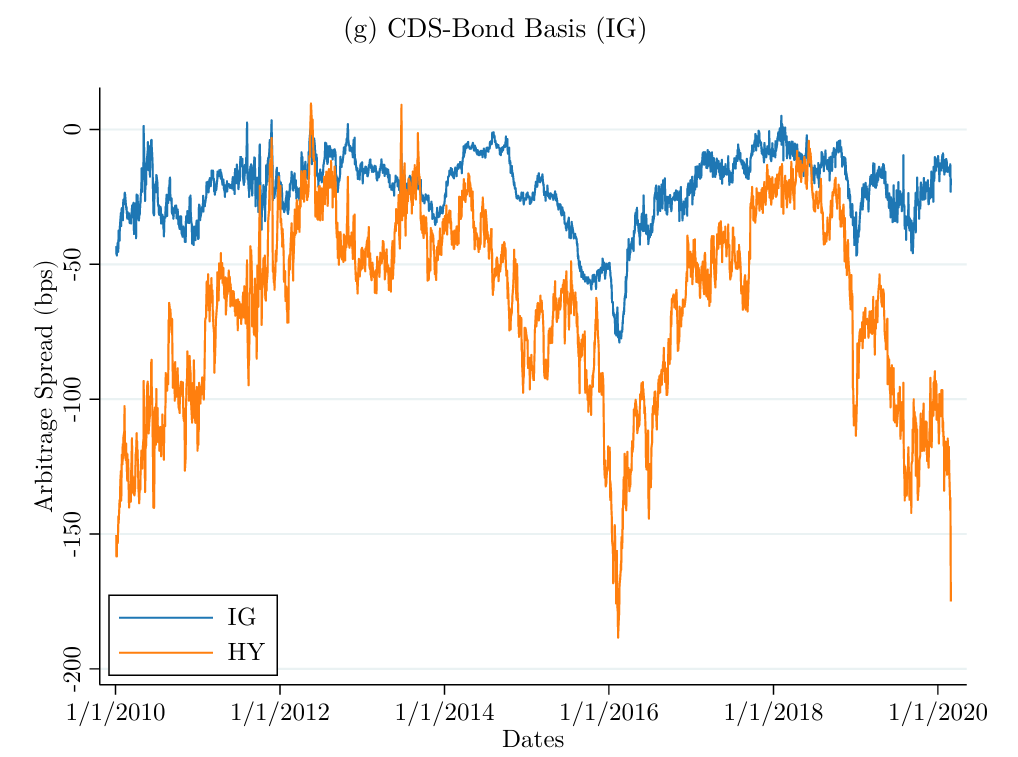
\includegraphics[width=.7\linewidth,height=210pt,width=350pt]{../docs_src/SegArb_CDS_Timeseries.png} \\[\abovecaptionskip]
%     \small (a) Findings in Siriwardane et al. (2023)
%   \end{tabular}

%   \vspace{\floatsep}

%   \begin{tabular}{@{}c@{}}
%     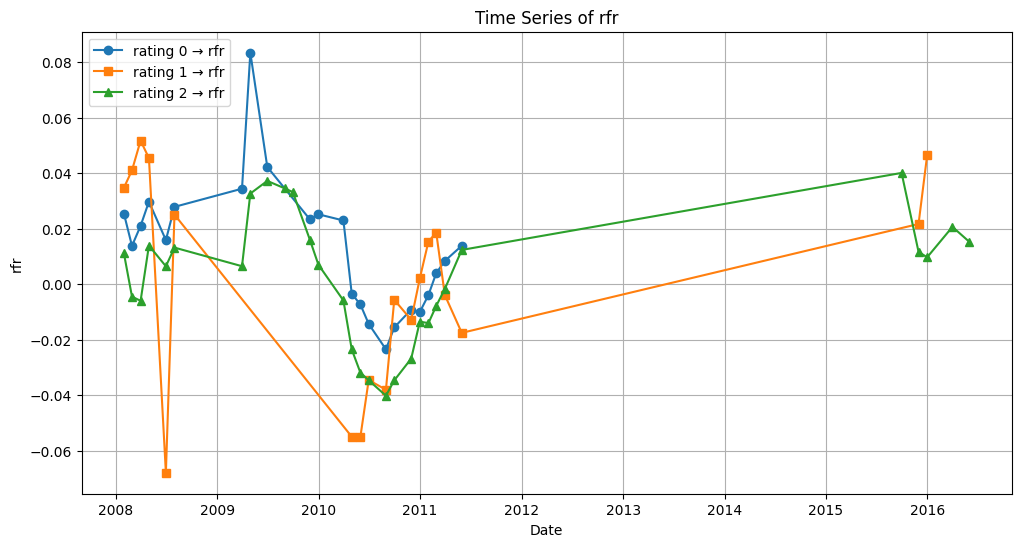
\includegraphics[width=.7\linewidth,height=200pt,width=400pt]{../docs_src/CDS_replicate.png} \\[\abovecaptionskip]
%     \small (b) Our findings
%   \end{tabular}

%   \caption{Comparison of CDS Arbitrage spreads}
%   \label{fig:CDS_replicate}
% \end{figure}


\begin{figure}
    \centering
    \begin{tabular}{@{}c@{}}
      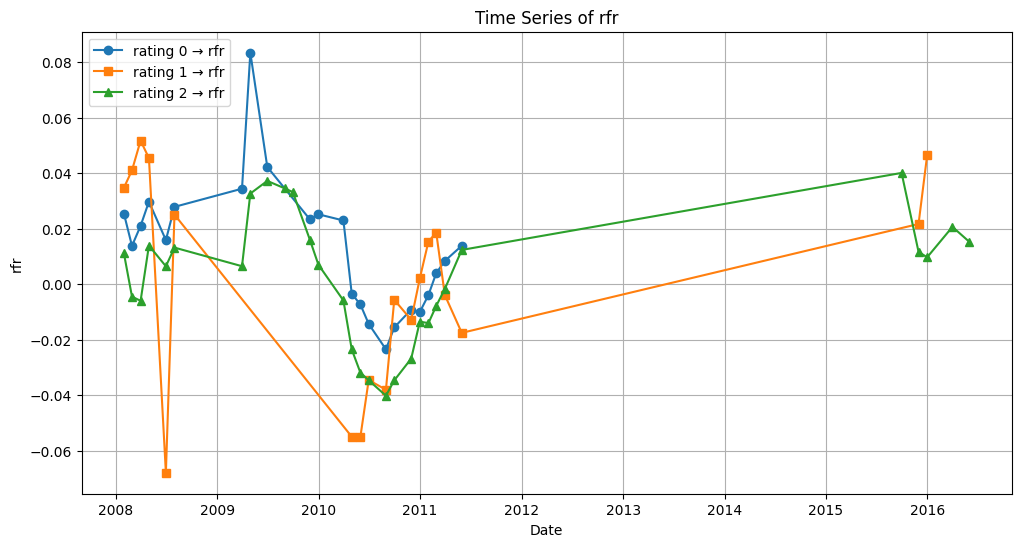
\includegraphics[width=.7\linewidth,height=200pt,width=400pt]{../docs_src/CDS_replicate.png}
    \end{tabular}
\caption{Comparison of CDS Arbitrage spreads}
\label{fig:CDS_replicate}
\end{figure}
  

\subsection{Additional Results}
\label{app:additional_results}
% Extended results tables and robustness checks

This section presents supplementary error metrics to provide a comprehensive view of model performance across all datasets. While the main text focuses on MASE and RMSE as primary metrics, we also report Symmetric Mean Absolute Percentage Error (sMAPE) and Mean Absolute Error (MAE) for completeness.

\subsubsection{Symmetric Mean Absolute Percentage Error (sMAPE)}

Table~\ref{tab:smape_results} presents sMAPE results across all model-dataset combinations. sMAPE provides percentage-based error measures that are symmetric and bounded, making them particularly useful for comparing performance across datasets with different scales and volatility patterns.

\begin{table}[htbp]
\centering
\caption{sMAPE Results by Dataset and Model}
\label{tab:smape_results}
% % sMAPE Results by Dataset and Model - tabular content only
% Generated automatically by create_results_tables2.py
\scriptsize
\setlength{\tabcolsep}{1.5pt}
\renewcommand{\arraystretch}{0.9}
\begin{tabular}{@{}lrrrrrrrrrrrr@{}}
\toprule
 & Naive & Theta & SES & ARIMA & DeepAR & NBEATS & NHITS & DLinear & NLinear & Transformer & TiDE & KAN \\
\midrule
\multicolumn{13}{l}{\textbf{Basis Spreads}} \\
CDS-Bond & 0.25 & 0.21 & 0.47 & 0.24 & 0.30 & 0.26 & 0.23 & 0.37 & \textbf{0.20} & 0.31 & 0.28 & 0.21 \\
CIP & 0.28 & 0.28 & 0.28 & \textbf{0.26} & 0.44 & 0.43 & 0.37 & 0.45 & 0.42 & 0.37 & 0.46 & 0.52 \\
TIPS-Treasury & 0.48 & 0.46 & 0.48 & 0.52 & 0.63 & \textbf{0.42} & 0.57 & 0.43 & 0.73 & 0.43 & 0.42 & 0.75 \\
\midrule
\multicolumn{13}{l}{\textbf{Returns (Portfolios)}} \\
CDS Portfolio & 0.17 & 0.13 & 0.13 & 0.13 & 0.12 & 0.12 & \textbf{0.12} & 0.12 & 0.15 & 0.13 & 0.12 & 0.13 \\
Corporate Portfolio & 1.58 & 1.56 & 2.92 & 2.04 & 1.27 & 2.18 & 1.69 & 1.52 & 1.30 & 1.46 & \textbf{1.13} & 1.22 \\
FF25 Size-BM & 3.44 & 2.31 & 1.12 & 2.12 & \textbf{1.04} & 1.80 & 3.39 & 1.39 & 1.59 & -- & 1.29 & 1.42 \\
SPX Options Portfolios & 0.70 & 3.85 & 0.70 & \textbf{0.68} & 0.73 & 0.77 & 0.70 & 0.70 & 0.75 & 0.77 & 9.85 & 0.72 \\
Treasury Portfolio & 2.83 & 1.36 & 2.98 & 3.65 & \textbf{1.31} & 537.67 & 2.91 & 2.83 & 2.05 & 2.19 & 2.00 & 14.34 \\
\midrule
\multicolumn{13}{l}{\textbf{Returns (Disaggregated)}} \\
CDS Contract & \textbf{0.15} & 0.16 & 0.16 & 0.57 & 0.58 & 0.76 & 0.22 & 0.25 & 0.26 & 0.18 & 0.40 & 0.20 \\
CRSP Stock & 3.25 & 1.34 & 1.26 & 1.32 & 1.83 & \textbf{1.22} & 1.59 & 1.44 & 8.35 & 1.25 & 1.38 & 1.42 \\
CRSP Stock (ex-div) & 3.29 & 1.44 & 1.33 & 1.29 & 3.03 & 1.66 & 1.35 & 4.94 & 2.04 & 1.23 & 1.24 & \textbf{1.13} \\
Commodity & 1.58 & \textbf{1.00} & \textbf{1.00} & 1.00 & 1.04 & 1.07 & 1.16 & 1.67 & 2.88 & 1.04 & 1.51 & 1.43 \\
Corporate Bond & 11.88 & 1.37 & 1.86 & 2.06 & \textbf{1.10} & 13.56 & 26.48 & 1.97 & 115.86 & 4.46 & 2.16 & 4.13 \\
FX & \textbf{0.82} & 0.90 & 0.82 & 0.92 & 0.83 & 0.90 & 0.95 & 1.29 & 0.88 & 0.94 & 0.94 & 0.87 \\
Treasury Bond & 1.16 & 1.83 & 1.73 & 1.00 & 0.81 & 1.03 & 1.20 & 10.50 & 0.76 & 2.94 & \textbf{0.41} & 0.83 \\
\midrule
\multicolumn{13}{l}{\textbf{Other}} \\
BHC Cash Liquidity & 0.17 & 0.16 & 0.16 & 0.17 & 0.19 & \textbf{0.16} & 0.16 & 0.20 & 0.18 & 0.16 & 0.19 & 0.16 \\
BHC Leverage & 0.04 & 0.04 & 0.04 & 0.04 & 0.08 & 0.03 & 0.03 & 0.05 & 0.04 & \textbf{0.03} & 0.04 & 0.04 \\
Bank Cash Liquidity & 0.18 & 0.18 & \textbf{0.17} & 0.19 & 0.21 & 0.17 & 0.17 & 0.21 & 0.20 & 0.17 & 0.20 & 0.18 \\
Bank Leverage & 0.04 & 0.04 & 0.04 & 0.04 & 0.14 & 0.04 & \textbf{0.04} & 0.06 & 0.04 & 0.04 & 0.05 & 0.04 \\
HKM All Factor & 0.77 & 0.95 & 0.82 & 0.72 & 2.61 & 1.01 & 3.13 & 0.93 & 0.74 & 1.51 & \textbf{0.69} & 24.22 \\
HKM Daily Factor & 0.62 & 2.05 & 2.31 & \textbf{0.56} & 2.19 & 10.47 & 2.97 & 4.49 & 3.58 & 2.49 & 1.68 & 2.31 \\
HKM Monthly Factor & 0.75 & 0.74 & 0.75 & 0.87 & 0.67 & 0.94 & 1.13 & \textbf{0.60} & 0.68 & 0.84 & 1.51 & 0.86 \\
Treasury Yield Curve & \textbf{0.22} & 0.31 & 0.22 & 0.49 & 0.23 & 0.49 & 0.57 & 0.23 & 0.23 & -- & -- & 0.55 \\
\bottomrule
\end{tabular}
\textit{SMAPE table unavailable: SMAPE data not present in current results.}
\vspace{0.1cm}

\noindent {\scriptsize \textbf{Note:} Values show Symmetric Mean Absolute Percentage Error (sMAPE). Lower values indicate better performance. -- indicates missing results.}
\end{table}

% Commented out: SMAPE heatmap unavailable since SMAPE data is not present
% Figure~\ref{fig:smape_heatmap} provides the corresponding visual representation of sMAPE results, making it easier to identify performance patterns and model consistency across different datasets.

% \begin{figure}[htbp]
% \centering
% \includegraphics[width=\textwidth]{../_output/forecasting/paper/smape_heatmap.png}
% \caption{sMAPE Results Heatmap by Dataset and Model. Colors are capped at the 90th percentile with extreme outliers marked by asterisks (*). The heatmap reveals percentage-based performance patterns, with cooler colors indicating better forecasting accuracy.}
% \label{fig:smape_heatmap}
% \end{figure}

\subsubsection{Mean Absolute Error (MAE)}

Table~\ref{tab:mae_results} shows MAE results for all combinations. MAE measures the average magnitude of errors in the original units, providing a straightforward interpretation of forecasting accuracy in terms of the actual data scale.

\begin{table}[htbp]
\centering
\caption{MAE Results by Dataset and Model}
\label{tab:mae_results}
% % MAE Results by Dataset and Model - tabular content only
% Generated automatically by create_results_tables2.py
\scriptsize
\setlength{\tabcolsep}{1.5pt}
\renewcommand{\arraystretch}{0.9}
\begin{tabular}{@{}lrrrrrrrrrrrr@{}}
\toprule
 & Naive & Theta & SES & ARIMA & DeepAR & NBEATS & NHITS & DLinear & NLinear & Transformer & TiDE & KAN \\
\midrule
\multicolumn{13}{l}{\textbf{Basis Spreads}} \\
CDS-Bond & \textbf{1.50} & 1.65 & 1.53 & 1.83 & 6.59 & 1.50 & 1.52 & 2.68 & 1.68 & 2.00 & 2.32 & 1.79 \\
CIP & 12.25 & 11.86 & 11.86 & \textbf{10.73} & 23.98 & 22.84 & 18.53 & 17.10 & 16.57 & 19.55 & 17.76 & 46.46 \\
TIPS-Treasury & 10.97 & 11.25 & 10.95 & 13.17 & 60.60 & 12.46 & \textbf{9.20} & 16.02 & 33.39 & 14.77 & 12.99 & 17.25 \\
\midrule
\multicolumn{13}{l}{\textbf{Returns (Portfolios)}} \\
CDS Portfolio & 0.00 & 0.00 & 0.00 & 0.00 & \textbf{0.00} & 0.00 & 0.00 & 0.00 & 0.00 & 0.00 & 0.00 & 0.00 \\
Corporate Portfolio & 0.02 & 0.02 & 0.02 & 0.02 & 0.02 & 0.02 & 0.02 & 0.02 & 0.02 & 0.02 & \textbf{0.02} & 0.02 \\
FF25 Size-BM & 0.01 & 0.01 & 0.01 & \textbf{0.01} & 0.01 & 0.01 & 0.01 & 0.01 & 0.01 & -- & 0.01 & 0.01 \\
SPX Options Portfolios & 0.02 & 0.02 & 0.02 & 0.02 & 0.02 & \textbf{0.02} & 0.02 & 0.02 & 0.02 & 0.02 & 0.02 & 0.02 \\
Treasury Portfolio & 0.00 & 0.00 & 0.00 & 0.00 & 0.00 & 0.00 & \textbf{0.00} & 0.00 & 0.00 & 0.00 & 0.00 & 0.00 \\
\midrule
\multicolumn{13}{l}{\textbf{Returns (Disaggregated)}} \\
CDS Contract & 0.00 & 0.00 & \textbf{0.00} & 0.00 & 0.01 & 0.00 & 0.00 & 0.00 & 0.00 & 0.00 & 0.00 & 0.00 \\
CRSP Stock & 0.24 & 0.24 & 0.23 & 0.22 & 0.21 & 0.22 & 0.23 & 0.22 & 0.19 & \textbf{0.19} & 0.20 & 0.20 \\
CRSP Stock (ex-div) & 0.24 & 0.24 & 0.23 & 0.22 & 0.21 & 0.23 & 0.23 & 0.22 & 0.19 & \textbf{0.19} & 0.20 & 0.20 \\
Commodity & 0.06 & 0.06 & 0.06 & \textbf{0.05} & 0.39 & 0.05 & 0.06 & 0.07 & 0.07 & 0.07 & 0.08 & 0.07 \\
Corporate Bond & 0.05 & \textbf{0.03} & 0.03 & 0.04 & 0.03 & 0.05 & 0.05 & 0.05 & 0.05 & 0.04 & 0.03 & 0.04 \\
FX & 1.79 & 2.00 & 1.79 & 1.96 & \textbf{1.72} & 1.92 & 2.08 & 1.89 & 1.92 & 1.86 & 1.85 & 2.05 \\
Treasury Bond & 0.01 & 0.01 & 0.01 & 0.01 & 0.01 & 0.01 & 0.01 & 0.01 & 0.01 & 0.01 & \textbf{0.00} & 0.01 \\
\midrule
\multicolumn{13}{l}{\textbf{Other}} \\
BHC Cash Liquidity & 0.02 & 0.02 & \textbf{0.02} & 0.02 & 0.03 & 0.02 & 0.02 & 0.03 & 0.03 & 0.02 & 0.03 & 0.02 \\
BHC Leverage & 0.70 & 0.74 & 0.70 & 0.75 & 1.61 & 0.67 & 0.68 & 1.01 & 0.78 & \textbf{0.66} & 0.76 & 0.71 \\
Bank Cash Liquidity & 0.03 & 0.03 & \textbf{0.03} & 0.03 & 0.04 & 0.03 & 0.03 & 0.04 & 0.03 & 0.03 & 0.04 & 0.03 \\
Bank Leverage & 0.70 & 0.70 & 0.70 & 0.79 & 3.13 & 0.67 & \textbf{0.67} & 1.13 & 0.81 & 0.70 & 0.96 & 0.72 \\
HKM All Factor & 71.28 & 78.12 & 71.28 & 70.32 & 72.31 & 74.13 & \textbf{50.73} & 67.95 & 69.80 & 67.54 & 68.05 & 56.20 \\
HKM Daily Factor & 18.61 & 26.97 & 18.61 & 18.51 & 20.05 & \textbf{18.36} & 18.73 & 19.07 & 18.76 & 22.44 & 18.92 & 18.62 \\
HKM Monthly Factor & 310.30 & 304.07 & 309.95 & 315.79 & 125.82 & 344.01 & 627.08 & 70.95 & 193.76 & 422.52 & \textbf{61.74} & 228.67 \\
Treasury Yield Curve & \textbf{0.96} & 1.22 & 0.96 & 1.81 & 0.98 & 1.74 & 1.96 & 0.99 & 0.97 & -- & -- & 1.93 \\
\bottomrule
\end{tabular}
\textit{MAE table unavailable: MAE data not present in current results.}
\vspace{0.1cm}

\noindent {\scriptsize \textbf{Note:} Values show Mean Absolute Error (MAE). Lower values indicate better performance. -- indicates missing results.}
\end{table}

Figure~\ref{fig:mae_heatmap} visualizes the MAE results, complementing the numerical table with clear visual patterns of absolute error magnitudes across all model-dataset combinations.

% \begin{figure}[htbp]
% \centering
% \includegraphics[width=\textwidth]{../_output/forecasting/paper/mae_heatmap.png}
% \caption{MAE Results Heatmap by Dataset and Model. Colors are capped at the 90th percentile with extreme values marked by asterisks (*). This visualization shows absolute error patterns in original data units, highlighting both model performance and relative dataset difficulty.}
% \label{fig:mae_heatmap}
% \end{figure}

% \section{Recyling Bin}
% % Temporary holding area for text that might not make it into the main text


% \subsection{The Consequences of Poor Data Quality in Analysis}
% \label{sec:consequences_of_poor_data_quality}
% An important feature of this paper, and the accompanying data repository, is that we provide a set of data that is cleaned and formatted in a way that matches best practices established within the corresponding academic literature. 
% Analyses based on incomplete, biased, or inconsistent datasets can lead to spurious results. For example, researchers in finance have documented several specific mechanisms by which poor data quality can mislead conclusions.

% \paragraph{Survivorship Bias}
% Perhaps the most cited data issue in performance studies, survivorship bias occurs when only surviving or successful entities in a dataset are observed, while failed or defunct entities are absent. This selective sampling can dramatically skew results.
% See \cite{Brown1992} or \cite{Brown1995} for seminal studies demonstrating that the apparent persistence or predictability in mutual fund returns was largely an artifact of survivorship bias.

% \paragraph{Selection and Instant History Bias}
% Related to survivorship bias are selection biases arising from how and when data are reported. In the context of hedge funds and other lightly regulated investments, researchers have noted that managers often have discretion over reporting, which can lead to instant history (backfill) bias. Instant history bias means that a fund might report its track record only after a streak of strong returns, effectively "backfilling" the database with only the good outcomes. This practice hides the early losses or failed ventures from view. See for example, \cite{Fung2000}, who found that accounting for backfill bias reduced average hedge fund returns by several percentage points per year.

% \paragraph{Measurement Errors}
% Even when all relevant cases are included, errors in the data itself (inaccurate measurements, typos, misclassifications, etc.) can bias results. In econometrics, it is well-established that classical measurement error in an independent variable will attenuate regression coefficients towards zero, masking true relationships. For instance, if a researcher uses an imperfect proxy or noisy measure of a firm's earnings, any estimated effect of earnings on stock returns will be biased downward (toward zero) due to the noise. Pioneering econometric analyses (e.g. \cite{Griliches1986} and \cite{Bound2001}) showed that measurement error can be a major source of bias, sometimes even more severe than omitted variable bias in certain cases.

% The mechanism is that the error in the explanatory variable gets absorbed into the regression's disturbance term, violating assumptions and leading to inconsistent estimates
% econ.lse.ac.uk
% . The consequence is that real economic signals may be drowned out by data noise. High-profile examples of measurement error causing spurious findings are sobering. A notable case involved Reinhart and Rogoff's influential study on public debt and growth \cite{Reinhart2010}, which concluded that countries with debt-to-GDP above 90% experience dramatically lower growth. When Herndon, Ash, and Pollin \cite{Herndon2014} attempted to replicate the result, they discovered coding errors and selective data exclusions in the original spreadsheet
% retractionwatch.com
% . These data issues, once corrected, entirely changed the conclusion: the sharp growth cliff at 90% debt largely disappeared
% retractionwatch.com
% . The Reinhart-Rogoff episode, documented in a subsequent published critique, revealed that a spreadsheet transcription error and omission of several countries' data had led to a false econometric result with far-reaching policy implications
% retractionwatch.com
% . This case underscores that even renowned studies can suffer from "garbage in" when data are mishandled --- and that replicating analysis with cleaned, corrected data is essential to validate findings.

% \paragraph{Non-Standard Definitions and Inconsistent Data}
% A more subtle problem arises when data are not standardized across sources or over time. If different companies or countries define metrics differently, any comparative analysis becomes apples-to-oranges. For example, in macroeconomics, price indices and GDP figures must be standardized (using purchasing power parity adjustments, consistent base years, etc.) to be meaningfully compared across countries. Summers and Heston \cite{Summers1991} demonstrated this by constructing the Penn World Table, a comprehensive set of national accounts data expressed in common terms
% econdata.com
% . Prior to their work, cross-country income comparisons were fraught with inconsistencies --- each nation's statistics were based on its own definitions and currencies. Summers and Heston's standardized data enabled economists to obtain unbiased comparisons of GDP and growth rates across ---
% econdata.com
% . The result was a wave of robust findings in growth economics that would have been impossible with non-standardized national data. Likewise, in finance, using current stock index membership to backtest historical performance (instead of using the actual historical index constituents at each point in time) introduces survivorship bias and inconsistency
% en.wikipedia.org
% en.wikipedia.org
% . An analysis that erroneously treats the present S\&P 500 members as if they existed in 1990 will ignore all the companies that were in the index then but failed later, thereby overstating historical returns
% en.wikipedia.org
% en.wikipedia.org
% . This highlights the importance of using data that are aligned to a common standard or definition appropriate to the analysis --- whether that means consistent accounting standards, index definitions, or economic variable calculations. Without such standardization, researchers may draw incorrect inferences simply because data series are not comparable.

% \paragraph{Spurious Correlations from Non-Stationarity}
% In time-series analysis, a classic data pitfall is using non-stationary (e.g. trending) data in regression without proper detrending or differencing. Granger and Newbold famously warned that regressing one growing time series on another can yield an apparently excellent fit (high R², significant t-statistics) that is actually spurious
% jumbong.github.io
% . They documented examples of nonsense correlations where two unrelated economic series, each with strong time trends, produced R² values near 0.99 and yet no meaningful relationship existed
% jumbong.github.io
% . In one case, they found a published regression with an astounding R² = 0.999 alongside a Durbin-Watson statistic of 0.09, indicating highly autocorrelated residuals --- a red flag for spurious regression
% jumbong.github.io
% . The lesson is that failing to transform or preprocess time-series data to stationarity can create illusory relationships driven by common trends rather than true causation. This problem is another form of "garbage in": if one feeds trending data into a linear model without precautions, the output will dutifully report a relationship (almost any two increasing series will correlate over time) --- an obvious garbage result. Modern econometric practice therefore emphasizes data preprocessing steps (taking logarithms, differences, removing trends or seasonality) to avoid such pitfalls. The need for these standardizing transformations is well supported by research. It has been shown that once data are rendered stationary and free of trend, spurious significance levels fall to normal rates
% jumbong.github.io
% . In sum, appropriate preprocessing of time-series (a form of standardization across time) is critical to obtaining reliable inference and not mistaking noise for signal.

% \paragraph{Data Snooping and Overfitting}
% A related concern in the realm of quantitative finance is data-snooping bias --- the false discoveries that occur when one mines a dataset for many possible patterns without proper adjustment. While this is more of a methodological issue than a data quality issue per se, it is worth noting as a cautionary tale that if one dredges "garbage data" hard enough, one will always find something. Sullivan, Timmermann, and White \cite{Sullivan1999} applied rigorous statistical checks to a large number of technical trading rules that had seemingly been profitable in past U.S. stock data. Publishing in the Journal of Finance, they showed that once one accounts for the fact that dozens of rules were tried (via White's Reality Check bootstrap), the vast majority of supposed "winning" trading strategies had no genuine predictive ---
% researchgate.net
% . Many earlier studies that lacked such corrections had overfit the data, effectively reporting noise as if it were a tradable signal
% researchgate.net
% . This reinforces the broader point: analyses conducted on poorly vetted or overly mined data can always produce some pattern of interest, but without out-of-sample validation or standardized methodologies, these are likely to be mirages. Ensuring data are partitioned properly (training vs. test sets, avoiding look-ahead bias where future information leaks into past data) is a form of maintaining data integrity in predictive modeling. The academic finance literature now contains countless factors and strategies discovered in historical data; however, as Harvey, Liu, and Zhu \cite{Harvey2016} argue in the Review of Financial Studies, many of these fail to hold up out-of-sample, suggesting that data-snooping and noise-fitting were at play. The community's response has been to demand higher standards of evidence (e.g. out-of-sample tests, multiple-comparison adjustments) --- essentially, more robust data handling --- before accepting new "discoveries." This again highlights how disciplined data practices filter out spurious results.---
% In all the above cases, the central theme is that poor data quality --- whether through biased sampling, inconsistent definitions, measurement error, or inadequate preprocessing --- can create false findings. These findings might look convincing (they may even be statistically significant or published in respected outlets), but they do not generalize or hold up under scrutiny because they are artifacts of faulty data. For researchers, analysts, and decision-makers, the implications are clear: one must critically assess data quality at the outset, or risk being led astray by garbage-in effects.


\end{appendices}

\end{document}